\section{Jet Energy Calibration}\label{sec:jec}

\subsection{Overview of the Calibration Strategy}

The purpose of the jet energy calibration is to relate, on average, the energy measured for the detector jet to the energy of the corresponding true particle jet. A true particle jet results from the clustering (with the same clustering algorithm applied to detector jets) of all stable particles originating from the fragmenting parton, as well as of the particles from the underlying event (UE) activity. The correction is applied as a multiplicative factor $\mathcal{C}$ to each component of the raw jet four-momentum vector $p_\mu^{raw}$ (components are indexed by $\mu$ in the following):

\begin{equation}
  \label{eq:master}
  p_\mu^{cor} = \mathcal{C}\cdot p_\mu^{raw}.
\end{equation}

The correction factor $\mathcal{C}$ is composed of the offset correction $C_\text{offset}$, the MC calibration factor $C_\text{MC}$, and the residual calibrations $C_\text{rel}$ and $C_\text{abs}$ for the relative and absolute energy scales, respectively. The offset correction removes the extra energy due to noise and pile-up, and the MC correction removes the bulk of the non-uniformity in $\eta$ and the non-linearity in \pt. Finally, the residual corrections account for the small differences between data and simulation. The various components are applied in sequence as described by the equation below:

\begin{equation}
  \label{eq:jec_components}
  \mathcal{C} = C_\text{offset}(\pt^{raw})\cdot C_\text{MC}(\pt^{\prime},\eta)\cdot C_\text{rel}(\eta)\cdot C_\text{abs}(\pt^{\prime\prime}),
\end{equation}

where $\pt^{\prime}$ is the transverse momentum of the jet after applying the offset correction and $\pt^{\prime\prime}$ is the \pt of the jet after all previous corrections. In the following sections, each component of the jet energy calibration will be discussed separately.

\subsection{Offset Correction}\label{sec:offset}

The offset correction is the first step in the chain of the factorized corrections. Its purpose is to estimate and subtract the energy not associated with the high-\pt scattering. The excess energy includes contributions from electronics noise and pile-up. In CMS, three approaches are followed for the offset correction: the jet area, the average offset and the hybrid jet area methods.

\subsubsection{Jet Area Method}

Recent developments in the jet reconstruction algorithms have allowed a novel approach for the treatment of pile-up~\cite{PU_JET_AREAS,JET_AREAS}: for each event, an average \pt-density $\rho$ per unit area is estimated, which characterizes the soft jet activity and is a combination of the underlying event, the electronics noise, and the pile-up. The two latter components contaminate the hard jet energy measurement and need to be corrected for with the offset correction.

The key element for this approach is the jet area $A_j$. A very large number of infinitely soft four-momentum vectors (soft enough not to change the properties of the true jets) are artificially added in the event and clustered by the jet algorithm together with the true jet components. The extent of the region in the $y-\phi$ space occupied by the soft particles clustered in each jet defines the active jet area. The other important quantity for the pile-up subtraction is the \pt density $\rho$, which is calculated with the $k_T$ jet clustering algorithm~\cite{KT1,KT2,KT3} with a distance parameter $R=0.6$. The $k_T$ algorithm naturally clusters a large number of soft jets in each event, which effectively cover the entire $y-\phi$ space, and can be used to estimate an average \pt-density. The quantity $\rho$ is defined on an event-by-event basis as the median of the distribution of the variable ${\pt}_j/A_j$, where $j$ runs over all jets in the event, and is not sensitive to the presence of hard jets. At the detector level, the measured density $\rho$ is the convolution of the true particle-level activity (underlying event, pile-up) with the detector response to the various particle types.

Based on the knowledge of the jet area and the event density $\rho$, an event-by-event and jet-by-jet pile-up correction factor can be defined:

\begin{equation}
\label{eq:fastjet}
  C_\text{area}(\pt^{raw},A_j,\rho) = 1-\frac{\left(\rho-\langle\rho_\text{UE}\rangle\right)\cdot A_j}{\pt^{raw}}.
\end{equation}

In the formula above, $\langle\rho_\text{UE}\rangle$ is the \pt-density component due to the UE and electronics noise, and is measured in events with exactly one reconstructed primary vertex (no pile-up). Figure~\ref{fig:fastjet} shows the PF \pt-density $\rho$, as a function of the leading jet \pt in QCD events and for various pile-up conditions. The fact that $\rho$ does not depend on the hard scale of the event confirms that it is really a measure of the soft jet activity. Finally, the density $\rho$ shows linear scaling properties with respect to the amount of pile-up.

\begin{figure}[ht!]
  \begin{center}
    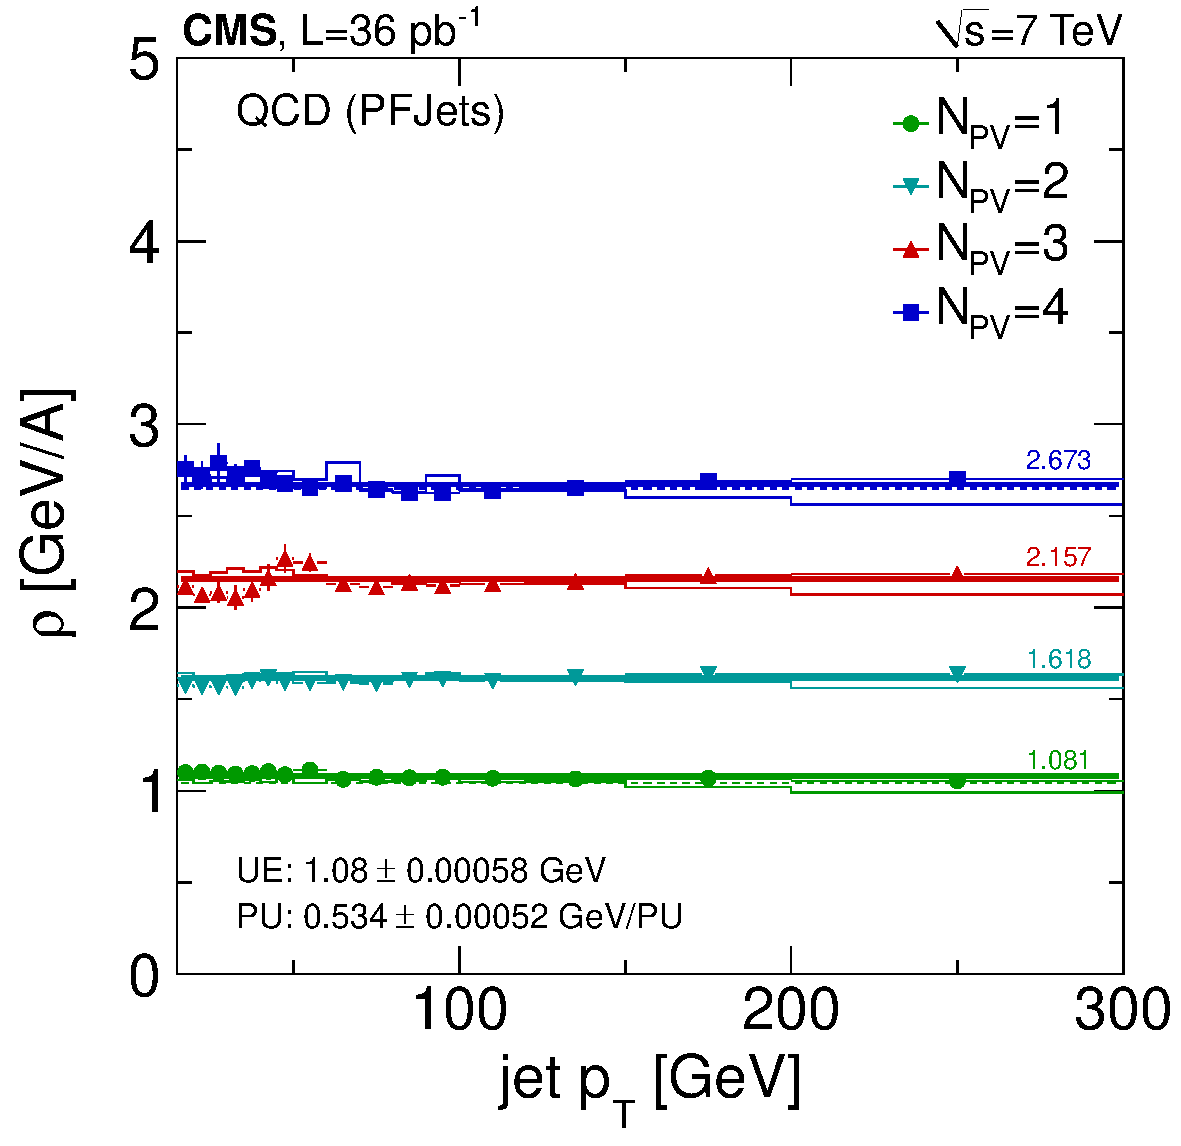
\includegraphics[width=0.45\textwidth]{Figures/JEC/QCD_RhoVsJet1Pt}
    \caption{Pile-up and underlying event PF \pt-density $\rho$, as a function of the leading jet \pt in the QCD multijet sample for various pile-up conditions (here $N_\text{PV}$ denotes the number of reconstructed vertices, and A denotes the unit area in the $y-\phi$ space).}
    \label{fig:fastjet}
  \end{center}
\end{figure}

\subsubsection{Average Offset Method}

The average offset method attempts to measure the average energy due to noise and pile-up, clustered inside the jet area, in addition to the energy associated with the jet shower itself. The measurement of the noise contribution is made in zero bias events by vetoing those that pass the minimum bias trigger. In the remaining events, the energy inside a cone of radius $R=0.5$ in the $\eta-\phi$ space is summed. The measurement is performed in cones centered at a specific $\eta$ bin and averaged across $\phi$. The noise contribution is found to be less than $250\MeV$ in \pt, over the entire $\eta$ range. The total average offset (over the entire dataset) is determined from inclusive zero bias events (with no veto on minimum bias triggers) and is classified according to the number of reconstructed vertices. Figure~\ref{fig:offset} shows the average offset \pt as a function of $\eta$ and for different pile-up conditions. The calorimetric offset \pt shows strong variations as a function of $\eta$, which follow the non-uniform particle response in the calorimeter, while for PF candidates, the offset \pt is more uniform versus $\eta$. The higher measured offset \pt for the PF-candidates is due to the much higher response with respect to the pure calorimetric objects. The observed $\eta$-asymmetry is related to calorimeter instrumental effects. For the highest number of vertices, in particular, the asymmetry is also of statistical nature (the adjacent points are highly correlated because at a given $\eta$ a large fraction of the energy in a cone of $R=0.5$ also ends up in overlapping cones). Figure~\ref{fig:PUcomposition} shows the breakdown, in terms of PF candidates, of the average offset \pt in events with one PU interaction, as measured in the data and compared to the MC prediction. The slight asymmetry observed in the MC is due to the asymmetric noise description in the specific version of the simulation. The average offset in \pt scales linearly with the number of reconstructed primary vertices, as shown in Fig.~\ref{fig:pileupPF}. The linear scaling allows the expression of the jet offset correction as follows:

\begin{equation}
  C_\text{offset}(\eta,\pt^{raw},N_\text{PV}) = 1-\frac{(N_\text{PV}-1)\cdot\mathcal{O}(\eta)}{\pt^{raw}},
\end{equation}

where $\mathcal{O}(\eta)$ is the average \pt due to one pile-up event, $\pt^{raw}$ is the \pt of the uncorrected jet, and $N_\text{PV}$ is the number of reconstructed primary vertices. The average offset method can be applied to jet algorithms that produce circular jets, while the quantity $\mathcal{O}(\eta)$ scales to larger cone sizes in proportion to the jet area. It should be noted that, in both the average offset subtraction and in the jet area method, the noise contribution and the UE are not subtracted. Because of the good description of the noise contribution in the simulation, the noise is taken into account with the MC-based correction.

\begin{figure}[ht!]
  \begin{center}
    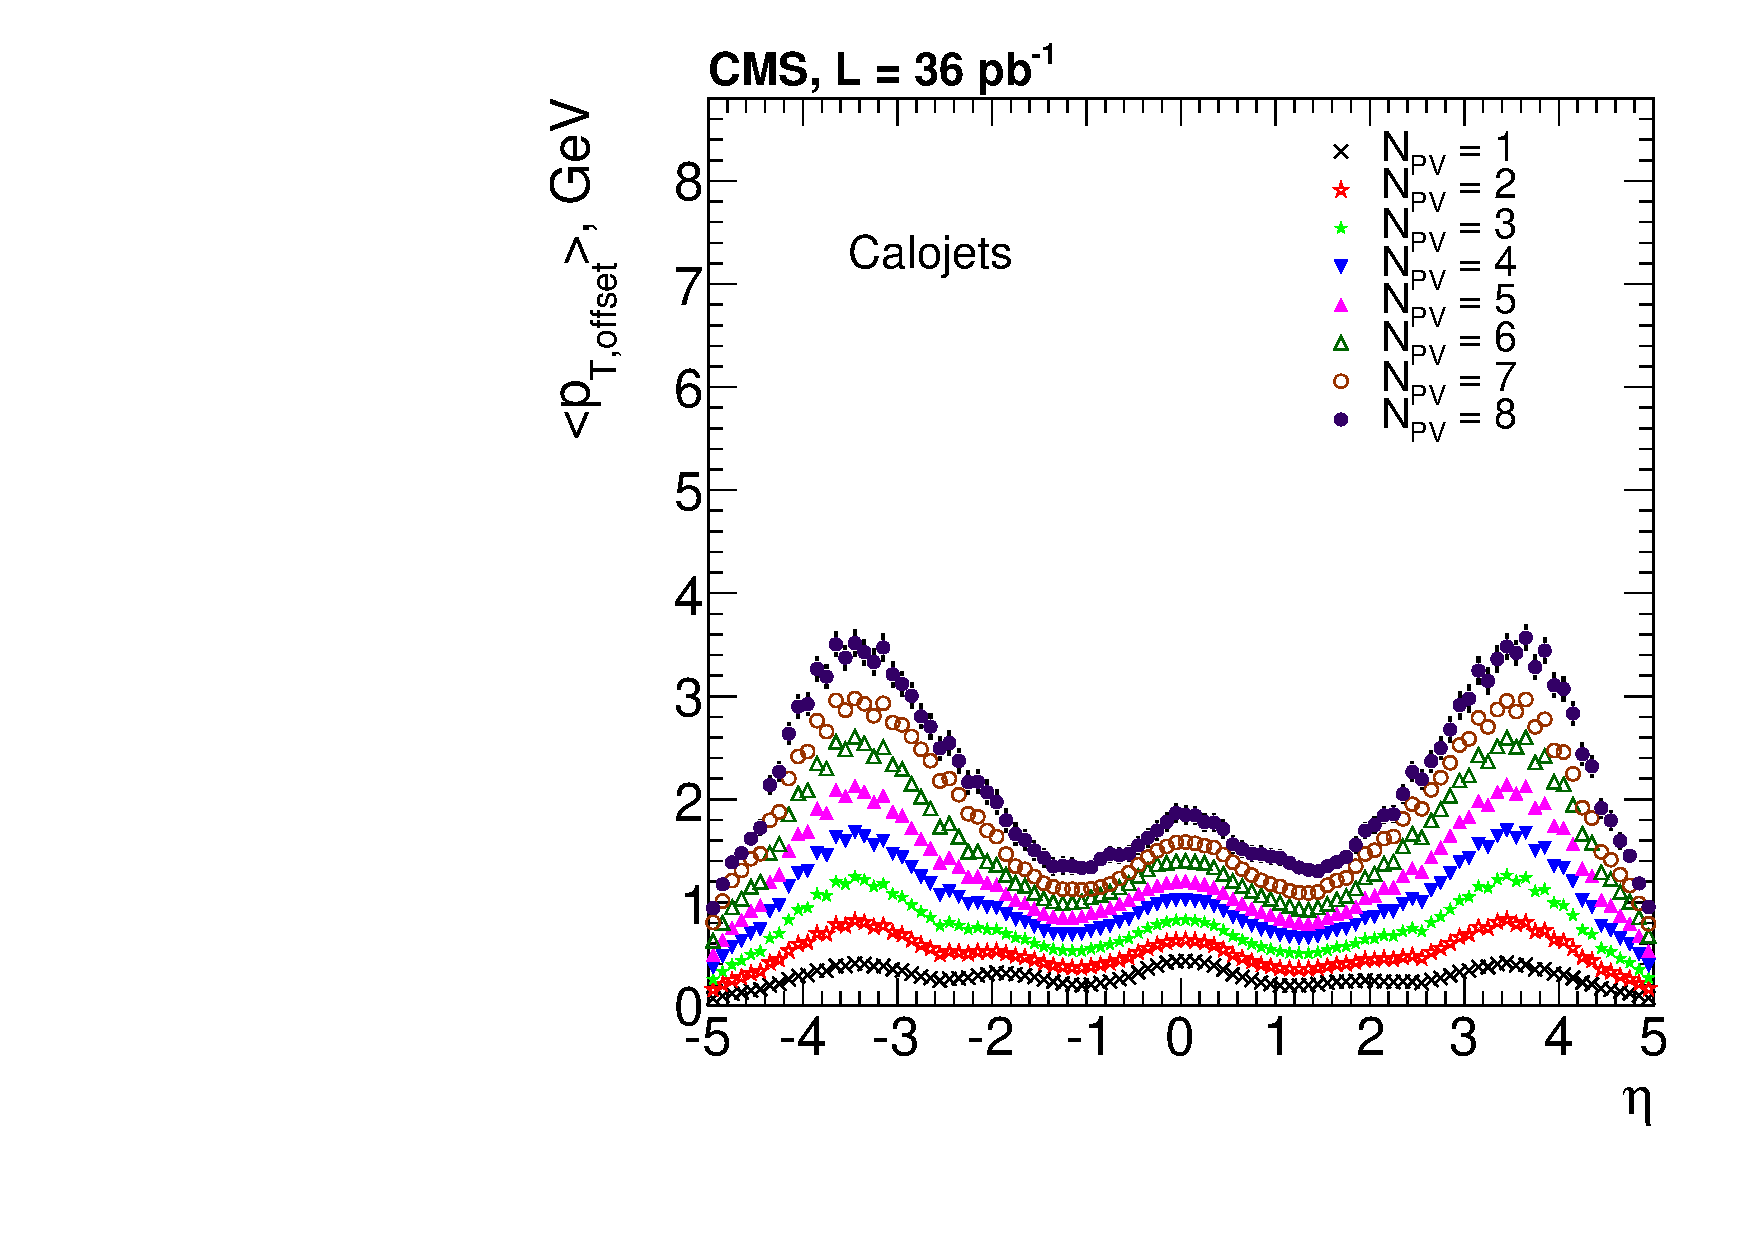
\includegraphics[width=0.45\textwidth]{Figures/JEC/p_AvgpTinC5_NoisePileup_PV_7TeV_run2010B_JNST}
    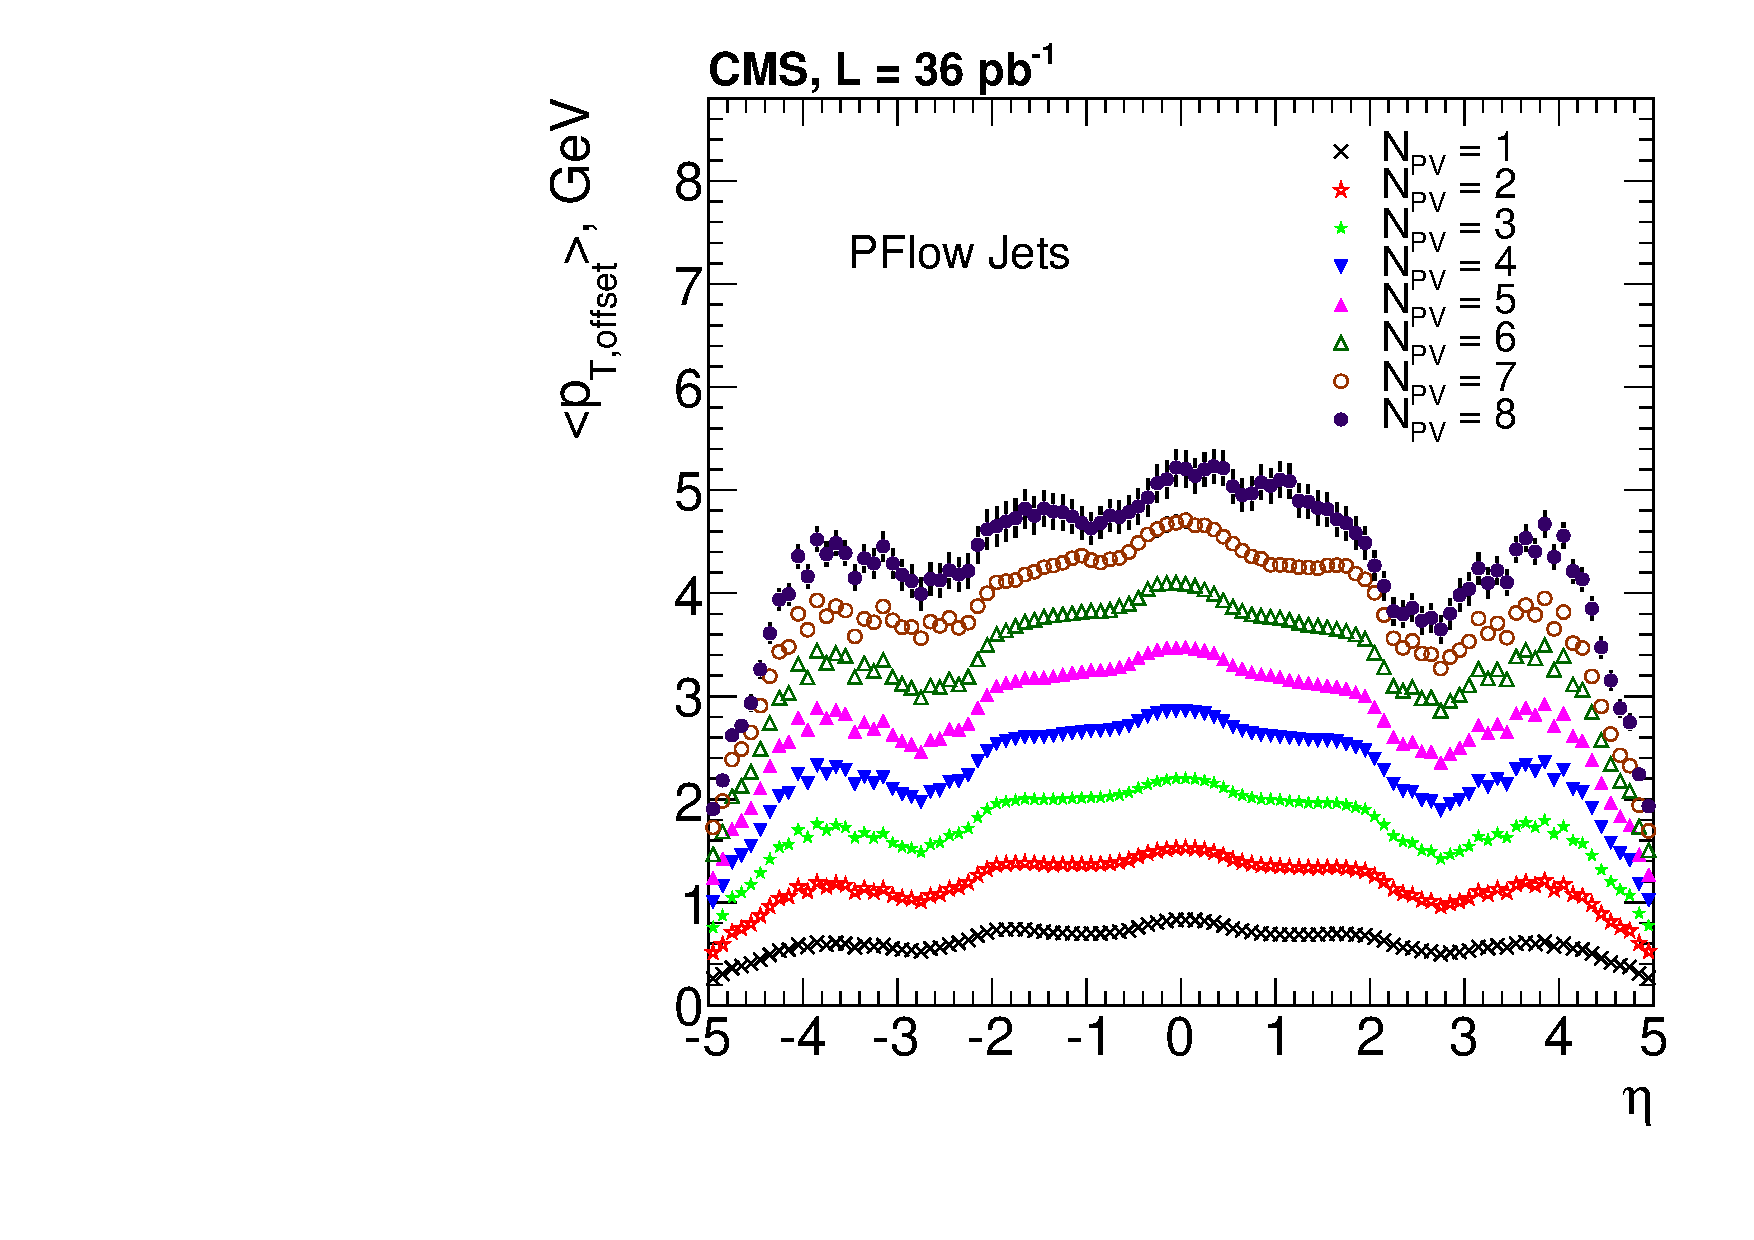
\includegraphics[width=0.45\textwidth]{Figures/JEC/p_AvgpTinPF5_NoisePileup_PV_7TeV_run2010B_JNST}
    \caption{Average offset in \pt, as a function of $\eta$, measured in minimum bias events for different pile-up conditions (categorized according to the number $N_\text{PV}$ of reconstructed primary vertices). Left: CALO jets. Right: PF jets.}
    \label{fig:offset}
  \end{center}
\end{figure}

\begin{figure}[ht!]
  \begin{center}
    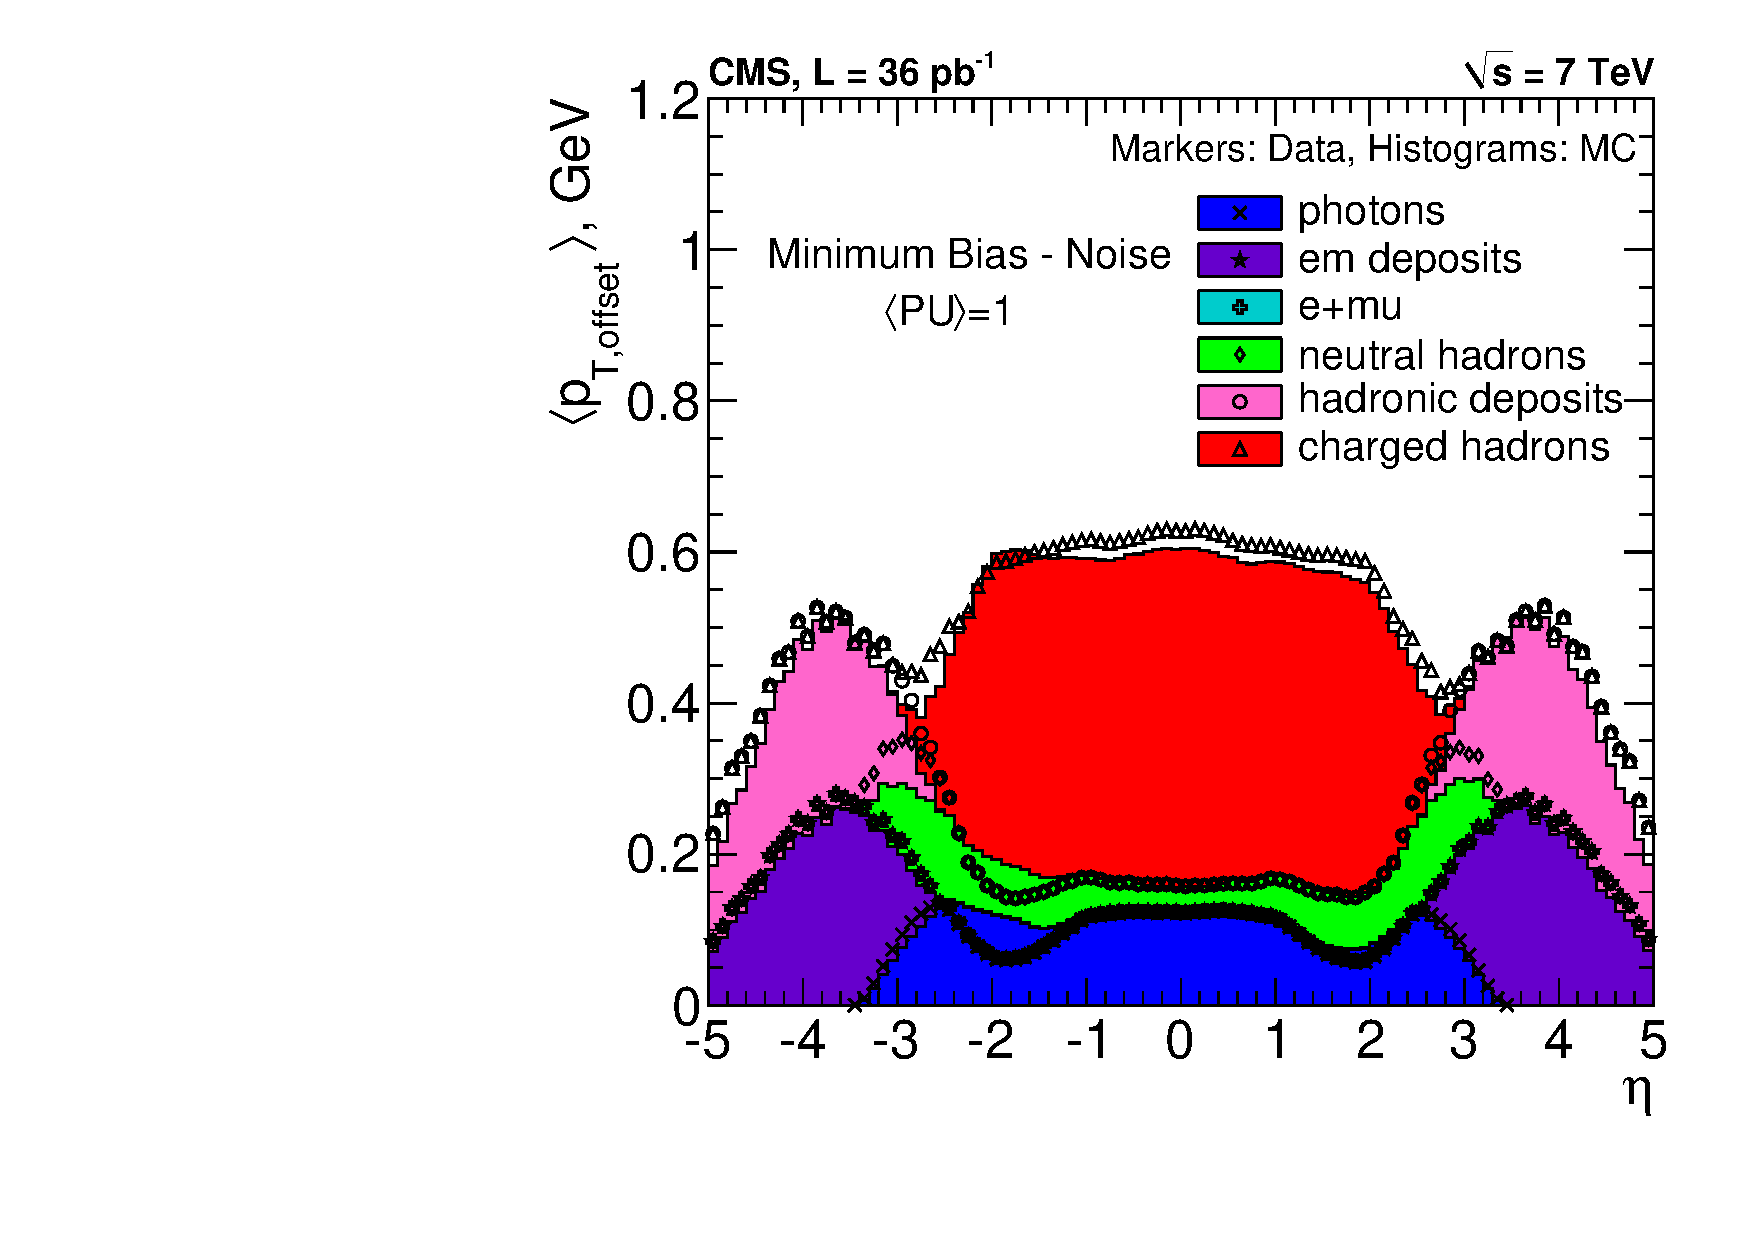
\includegraphics[width=0.45\textwidth]{Figures/JEC/h_AvgpTinPF5_stacked_MinBiasMinusZB}
    \caption{Breakdown of the average offset \pt, in terms of the PF candidates, as a function of $\eta$, for events with one PU interaction. Data are shown by markers and MC is shown as filled histograms.}
    \label{fig:PUcomposition}
  \end{center}
\end{figure}

\begin{figure}[ht!]
  \begin{center}
    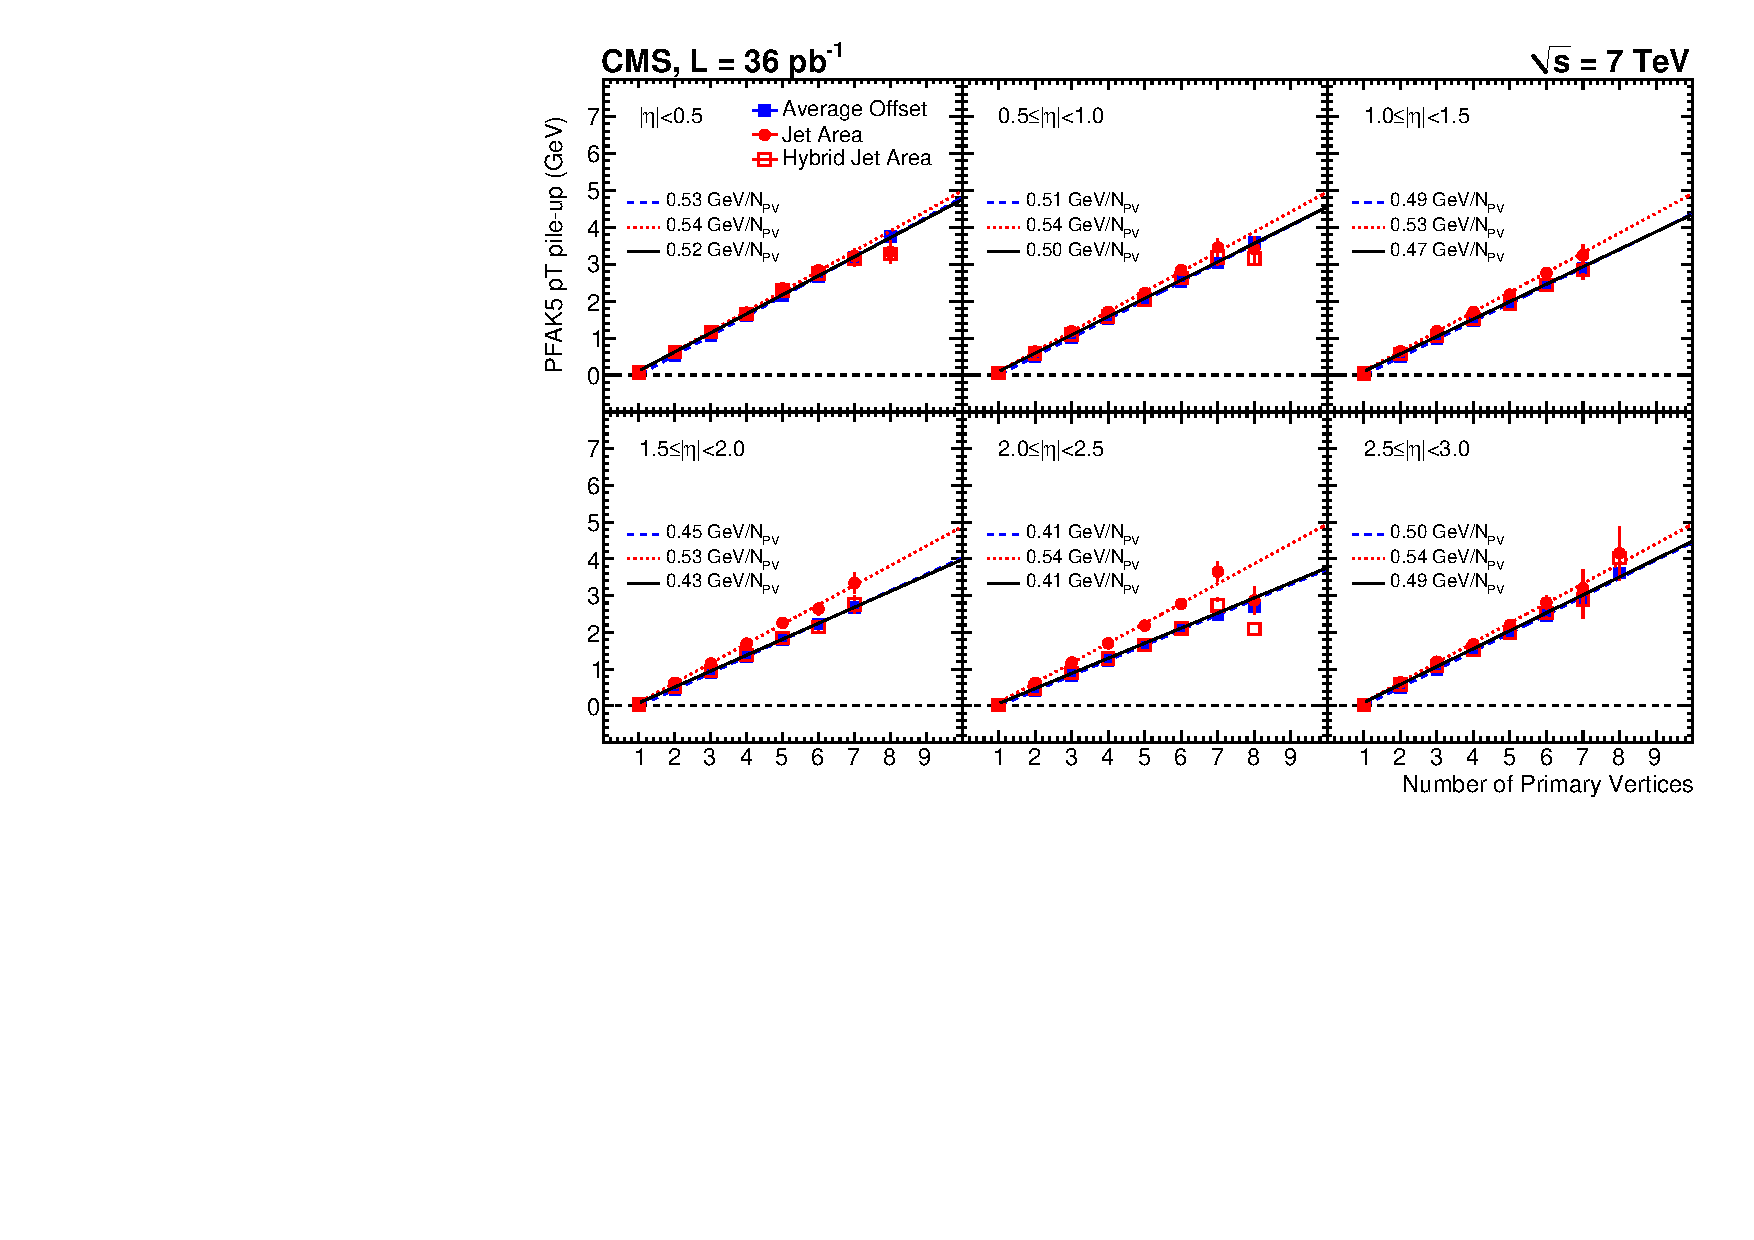
\includegraphics[width=0.9\textwidth]{Figures/JEC/PileUpComparison_NoPFNoPU_PF}
    \caption{Average PF jet pile-up \pt, as a function of the number of reconstructed vertices ($N_\text{PV}$) for the jet area, the average offset, and the hybrid jet area methods in 6 different $\eta$ regions. In the y-axis title, PFAK5 denotes the PF jets reconstructed with the anti-$k_T$ algorithm with distance parameter $R=0.5$.}
    \label{fig:pileupPF}
  \end{center}
\end{figure}

\subsubsection{Hybrid Jet Area Method}

The measurement of the average offset presented in the previous paragraph confirms the $\eta$-dependence of the offset energy. This is explained by the fact that the measured offset is the convolution of the pile-up activity with the detector response. In order to take into account the $\eta$-dependence, a hybrid jet area method is employed:

\begin{equation}
\label{eq:hybrid}
  C_\text{hybrid}(\pt^{raw},\eta,A_j,\rho) = 1-\frac{(\rho-\langle\rho_\text{UE}\rangle)\cdot\beta(\eta)\cdot A_j}{\pt^{raw}}.
\end{equation}

In Eq.~(\ref{eq:hybrid}), the \pt density $\rho$ and the corresponding density due to the UE, $\langle\rho_{UE}\rangle$ are constants over the entire $\eta$ range. The multiplicative factor $\beta(\eta)$ corrects for the non-uniformity of the energy response and is calculated from the modulation of the average offset in \pt (Fig.~\ref{fig:offset}).

In the case of PF jets, the response variation versus $\eta$ is relatively small and the hybrid jet area method is found to be in excellent agreement with the average offset method. Figure~\ref{fig:pileupPF} shows the average offset in \pt as a function of the number of reconstructed primary vertices, for the three different methods (jet area, average offset, hybrid jet area). It can be seen that the differences between the jet area method and the average offset method are entirely due to the response dependence on $\eta$. The hybrid jet area method is chosen for the pile-up correction of PF jets. In the case of CALO jets, and also JPT jets (initially reconstructed as CALO jets), the response variation versus $\eta$ shows dramatic changes and neither the simple jet area nor the hybrid jet area methods are able to reproduce the average offset measurement. Therefore, for CALO jets, the average offset method is the one chosen for the pile-up correction.

\subsubsection{Offset Uncertainty}\label{sec:offset_unc}

The uncertainty of the offset correction is quantified using the jet area method. Specifically, the quantities $\rho$ and $\langle\rho_\text{UE}\rangle$ in Eq.~(\ref{eq:fastjet}) are varied independently and the resulting shifts are added in quadrature. The event \pt-density $\rho$ uncertainty is estimated as $0.2\GeV$ per unit jet area and per pile-up event. This uncertainty is based on the maximum slope difference between the jet area and the average offset methods, and the residual non-closure in the average offset method. The UE \pt-density $\langle\rho_\text{UE}\rangle$ uncertainty is estimated as $0.15\GeV$ per unit jet area, based on the differences observed between the QCD multijet and Z+jets samples, and on the effective difference when applied in the inclusive jet cross-section measurement. Figure~\ref{fig:offsetUnc} shows the uncertainty of the offset correction, as a function of jet \pt and the number of primary vertices.

\begin{figure}[ht!]
  \begin{center}
    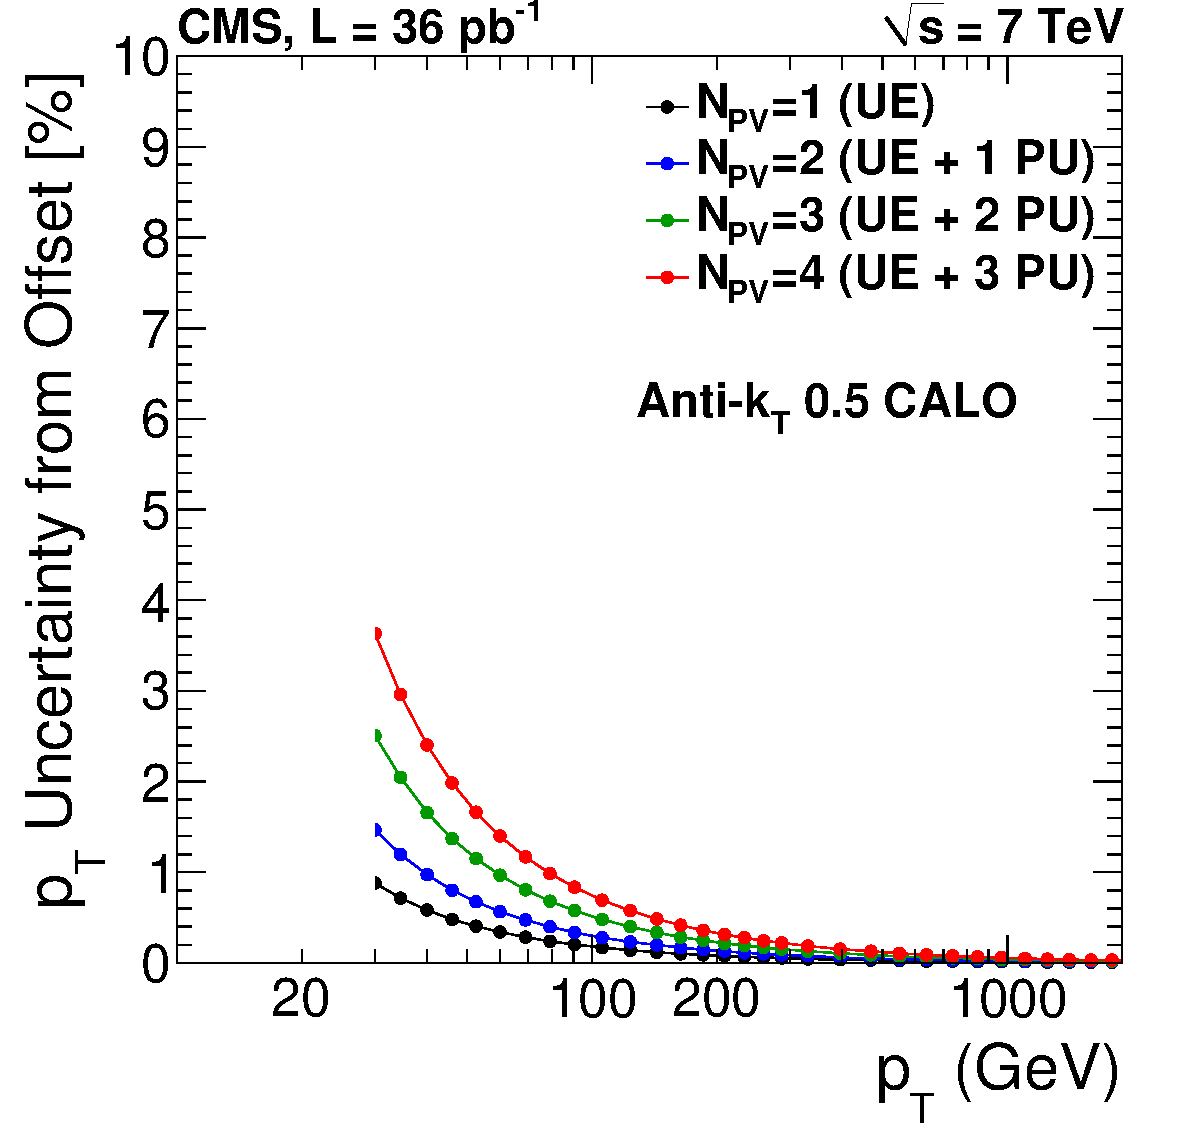
\includegraphics[width=0.45\textwidth]{Figures/JEC/JECUncert_Offset_CALOAK5.pdf}
    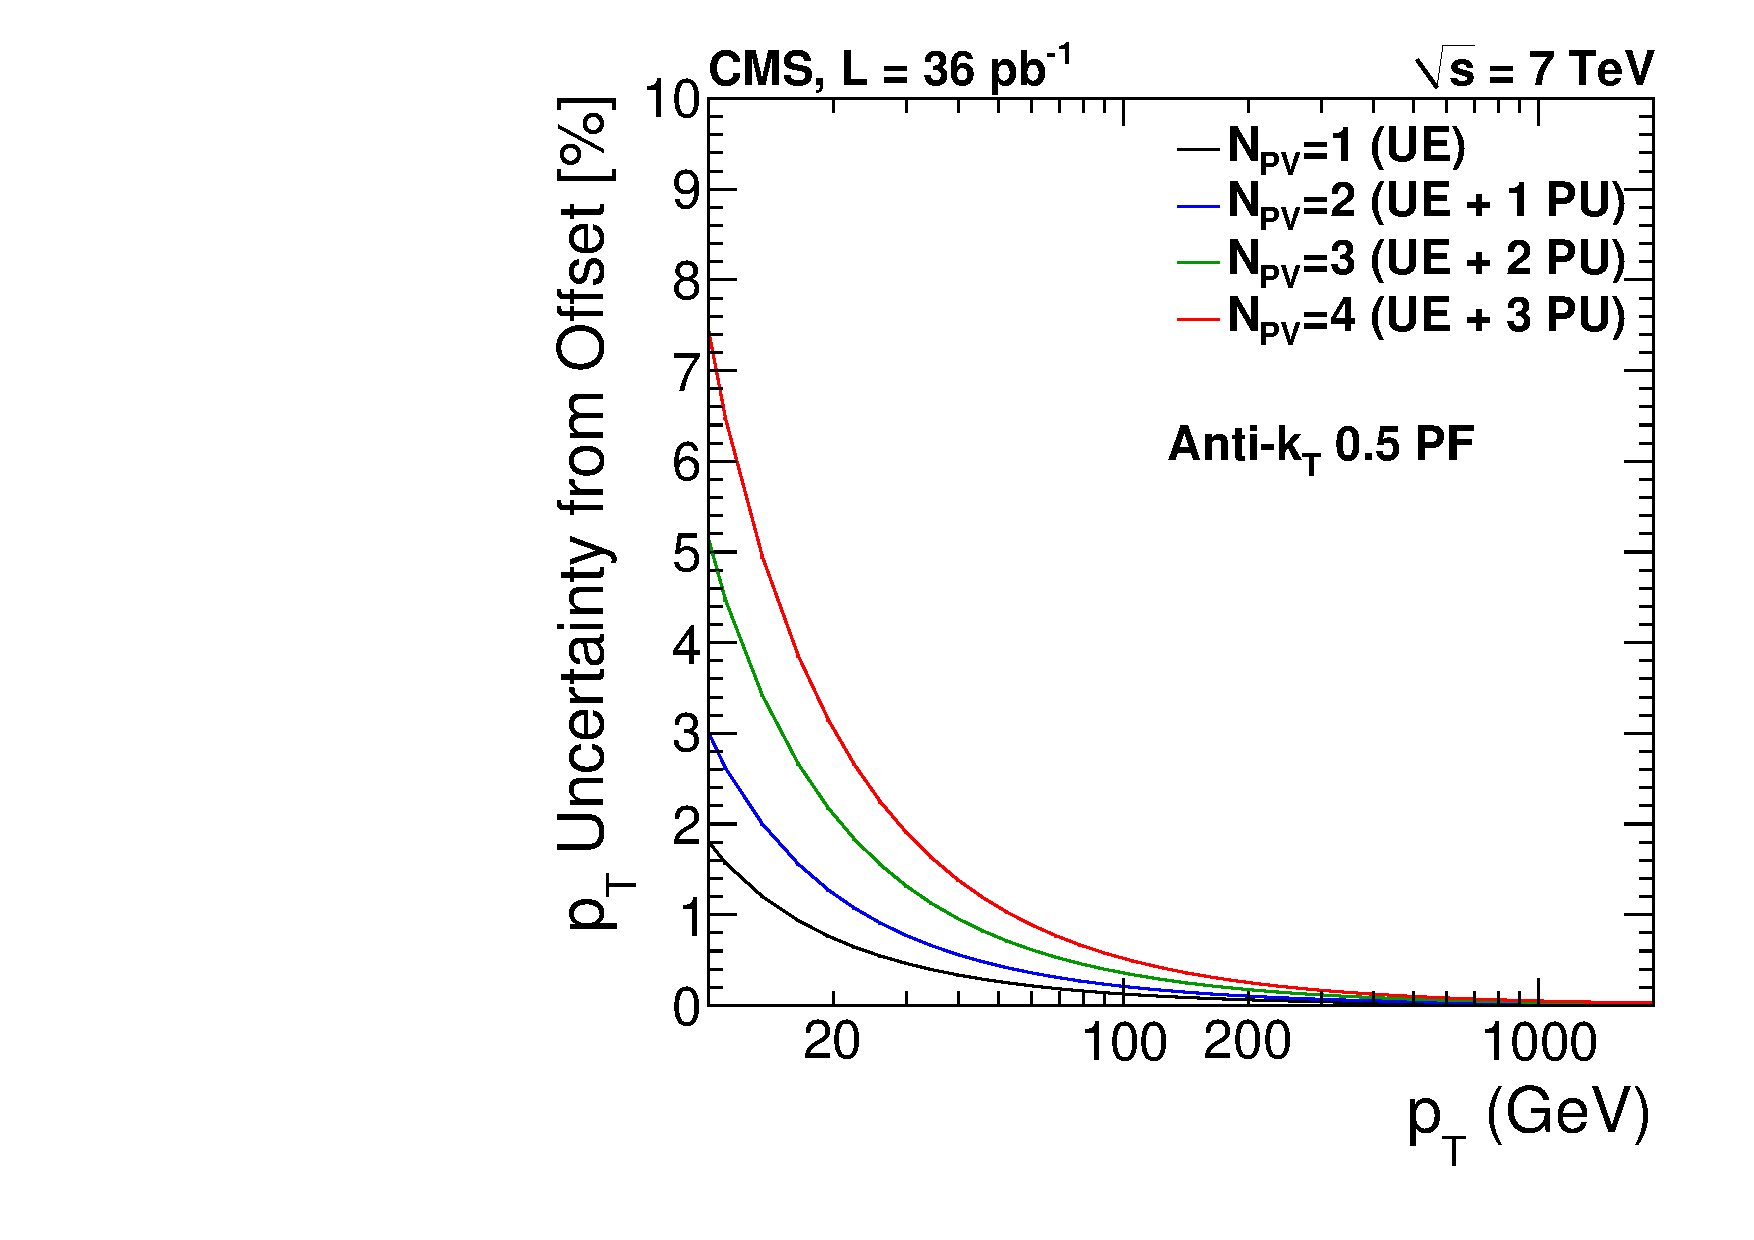
\includegraphics[width=0.45\textwidth]{Figures/JEC/JECUncert_Offset_PFAK5.pdf}
    \caption{Offset jet-energy-correction uncertainty as a function of jet \pt. Left: CALO jets. Right: PF jets.}
    \label{fig:offsetUnc}
  \end{center}
\end{figure}


\subsection{Monte Carlo Calibration}

The MC calibration is based on the simulation and corrects the energy of the reconstructed jets such that it is equal on average to the energy of the generated MC particle jets. Simulated QCD events are generated with {\sc PYTHIA}6.4.22~\cite{PYTHIA}, tune Z2 (the {\sc Z2} tune is identical to the {\sc Z1} tune described in~\cite{D6T} except that {\sc Z2} uses the CTEQ6L PDF, while {\sc Z1} uses CTEQ5L) and processed through the CMS detector simulation, based on {\sc GEANT4}~\cite{GEANT4}. The jet reconstruction is identical to the one applied to the data. Each reconstructed jet is spatially matched in the $\eta-\phi$ space with a MC particle jet by requiring $\Delta R<0.25$. In each bin of the MC particle transverse momentum $\pt^{gen}$, the response variable $\mathcal{R}=\pt^{reco}/\pt^{gen}$ and the detector jet $\pt^{reco}$ are recorded. The average correction in each bin is defined as the inverse of the average response $C_\text{MC}(\pt^{reco})=\frac{1}{<\mathcal{R}>}$, and is expressed as a function of the average detector jet \pt $<\pt^{reco}>$. Figure~\ref{fig:mctruthVsEta} shows the MC jet energy correction factor for the three jet types, vs. $\eta$, for different corrected jet \pt values. Figure~\ref{fig:mctruthVsPt} shows the average correction in $|\eta|<1.3$, as a function of the corrected jet \pt.

Calorimeter jets require a large correction factor due to the non-linear response of the CMS calorimeters. The structures observed at $|\eta|\sim 1.3$ are due to the barrel-endcap boundary and to the tracker material budget, which is maximum in this region. The fast drop observed in the endcap region $1.3<|\eta|<3.0$ is due to the fact that the jet energy response depends on energy rather than on jet \pt. For higher values of $|\eta|$ more energy corresponds to a fixed \pt value $E\approx\pt\cdot\cosh(\eta)$, which means that the jet response is higher and the required correction factor is smaller. The structure observed at $|\eta|\sim 3.0$ coincides with the boundary between the endcap and the forward calorimeters. Finally, in the region $|\eta|>4.0$, the jet energy response is lower because parts of the jets pointing toward this region extend beyond the forward calorimeter acceptance.

The track-based jet types (JPT and PF) require much smaller correction factors because the charged component of the jet shower is measured accurately in the CMS tracker which extends up to $|\eta|=2.4$. The fast rise of the correction factor for JPT jets in the region $2.0<|\eta|<2.5$ is explained by the fact that part of the jets lying in this region extends beyond the tracker coverage. For PF jets, the transition beyond the tracker acceptance is smoother because the PF candidates, which are input to the clustering of PF jets, are individually calibrated prior to the clustering. While both PF jets and JPT jets exploit the tracker measurements, the JPT jets require lower correction in the region $|\eta|<2.0$ because the tracker inefficiency is explicitly corrected for by the JPT algorithm.
In the forward region ($|\eta|>3.0$) all three jet types converge to simple calorimetric objects and therefore require almost identical corrections.

\begin{figure}[ht!]
  \begin{center}
    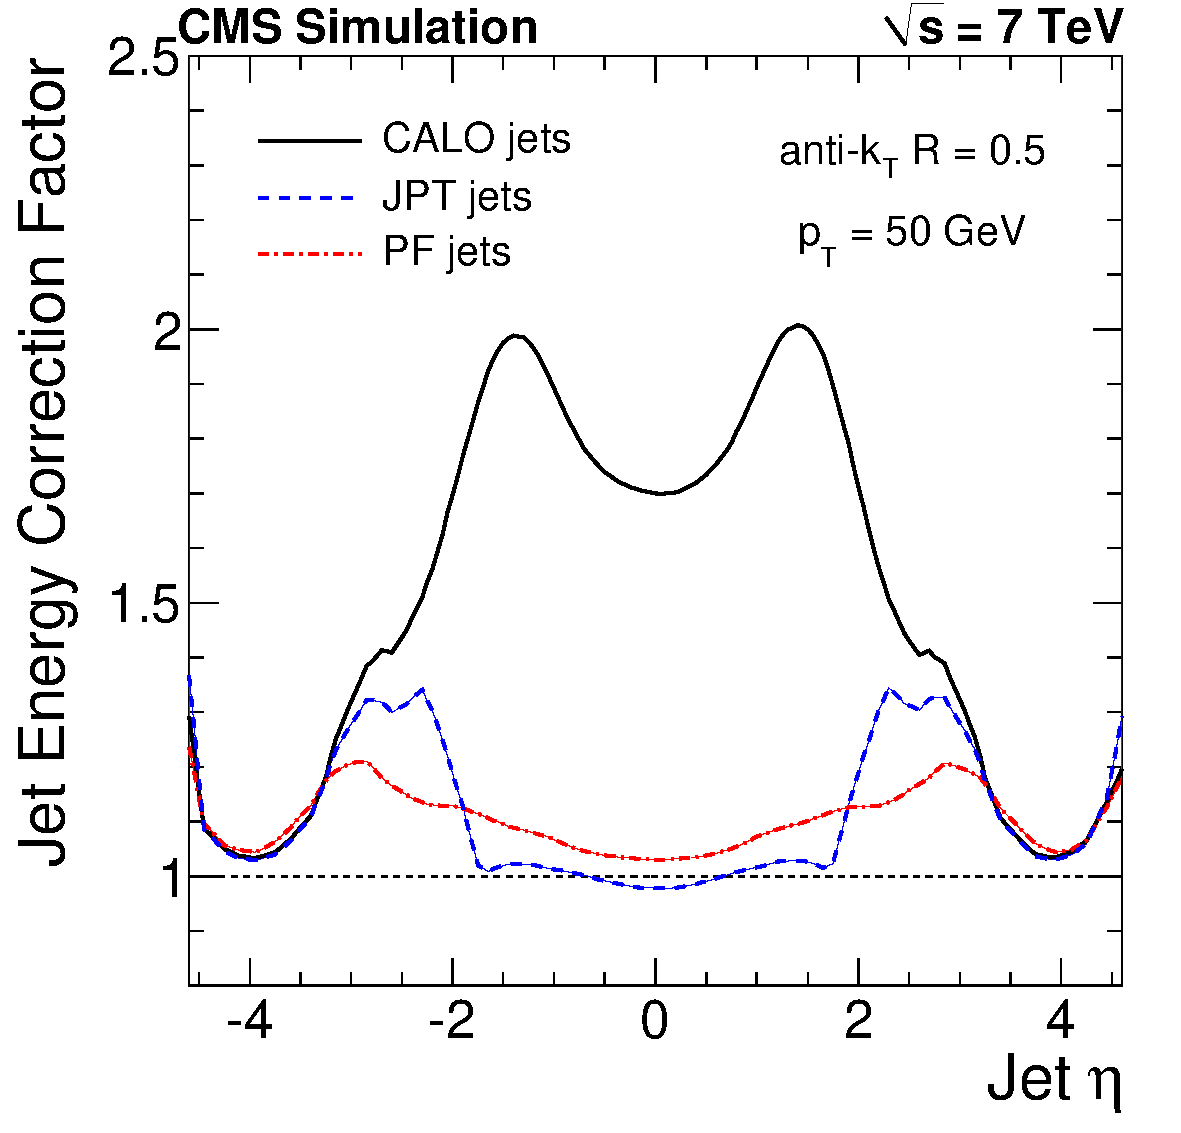
\includegraphics[width=0.45\textwidth]{Figures/JEC/JEC_MCtruth_vs_Eta_CorPt50}
    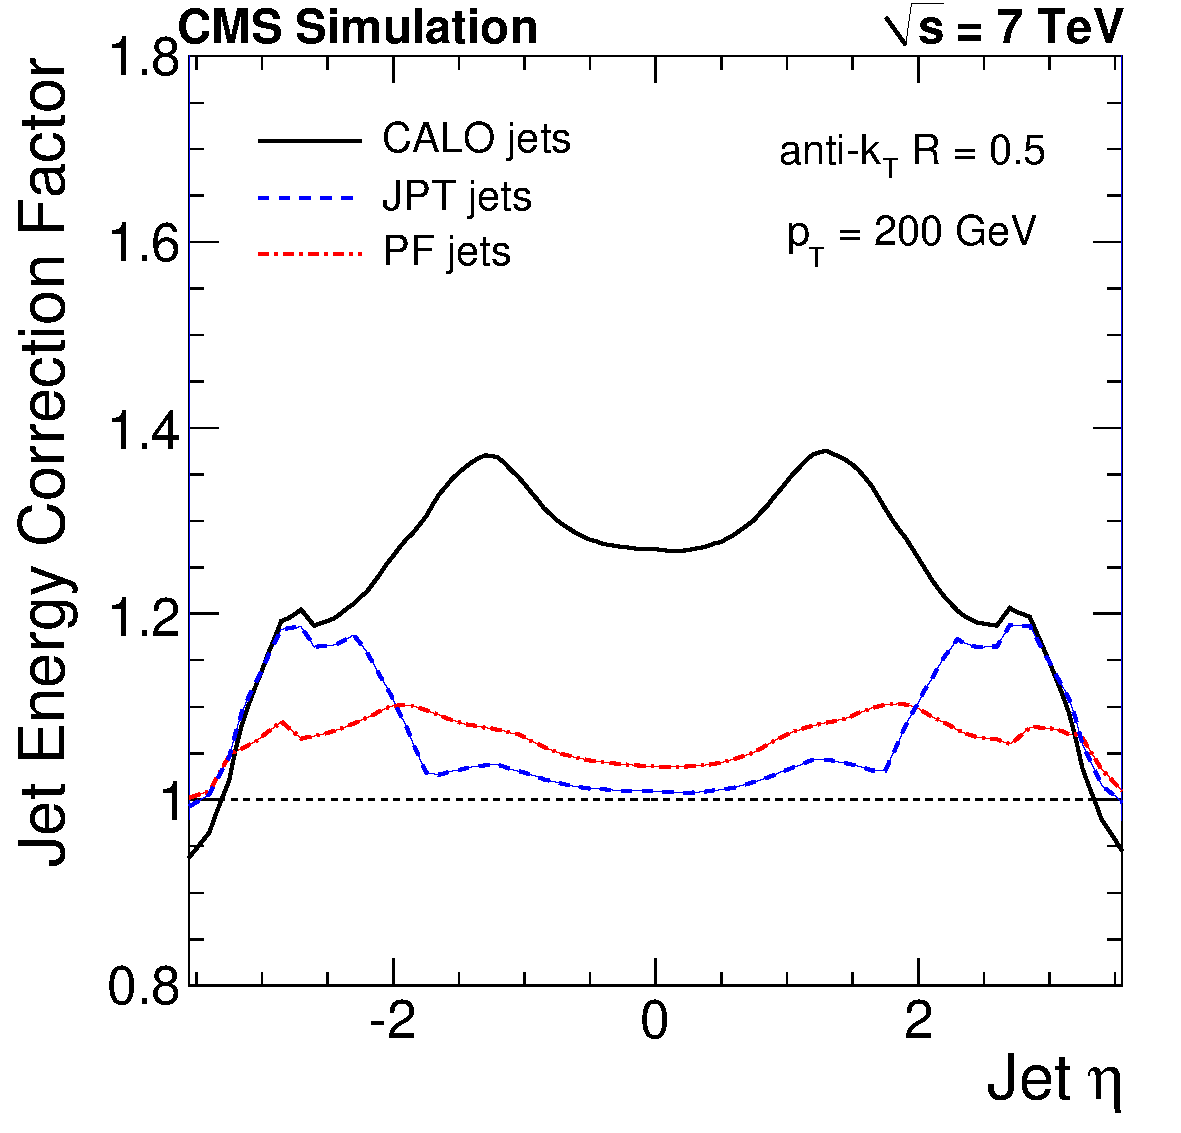
\includegraphics[width=0.45\textwidth]{Figures/JEC/JEC_MCtruth_vs_Eta_CorPt200}
    \caption{Monte Carlo jet-energy-correction factors for the different jet types, as a function of jet $\eta$. Left: correction factor required to get a corrected jet $\pt=50\GeV$. Right: correction factor required to get a corrected jet $\pt=200\GeV$.}
    \label{fig:mctruthVsEta}
  \end{center}
\end{figure}

\begin{figure}[ht!]
  \begin{center}
    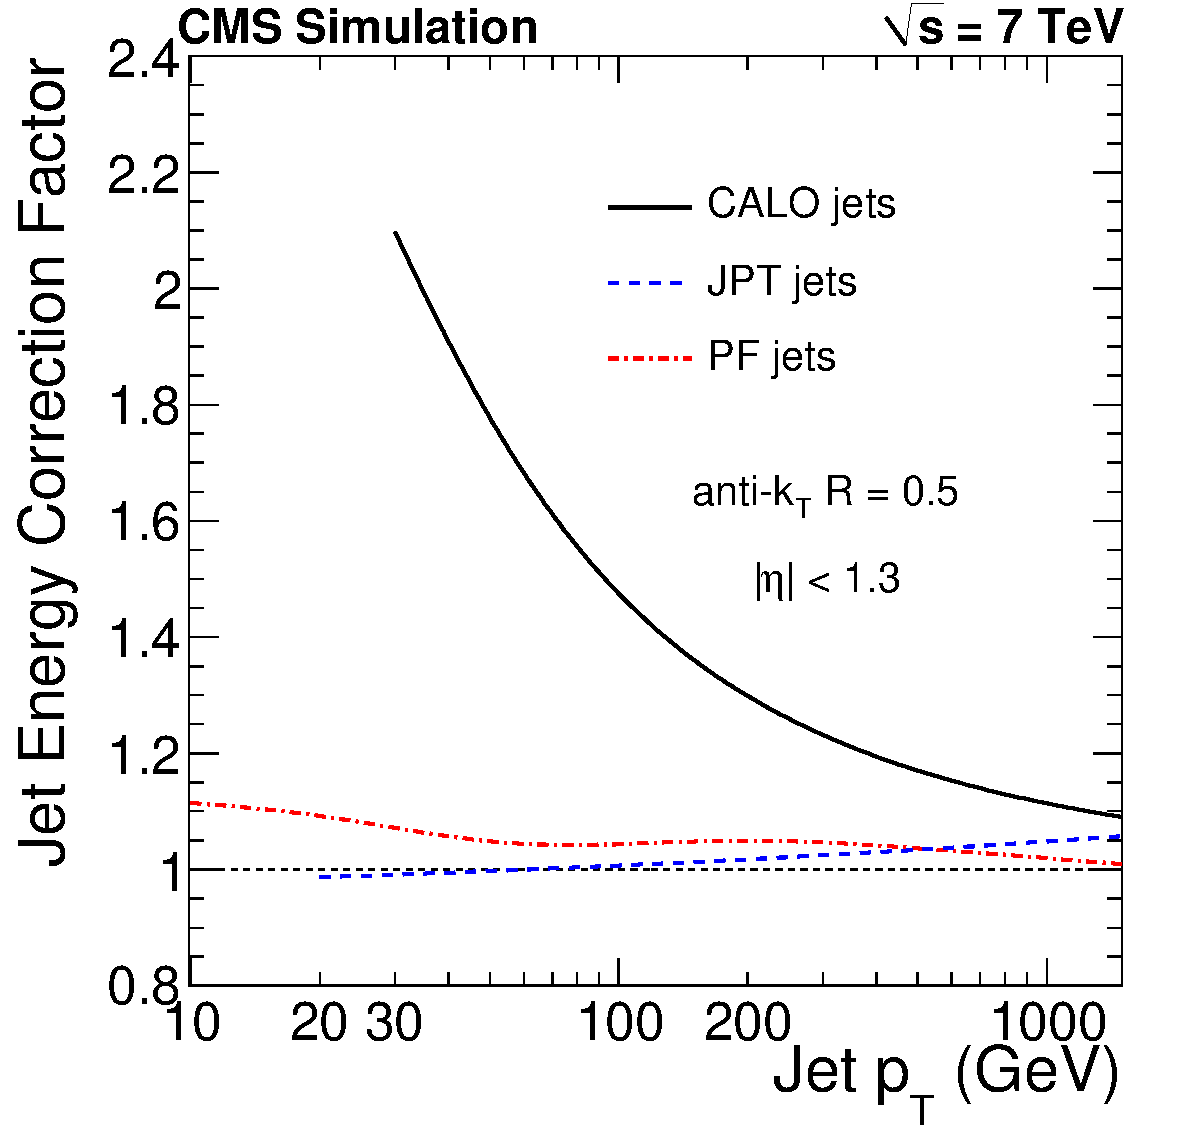
\includegraphics[width=0.45\textwidth]{Figures/JEC/JEC_MCtruth_vs_CorPt_Barrel}
    \caption{Monte Carlo jet-energy-correction factors for the different jet types, as a function of jet \pt.}
    \label{fig:mctruthVsPt}
  \end{center}
\end{figure}

The default MC calibration is derived from the QCD sample and corresponds to a jet flavour composition enriched in low-\pt gluon jets. The jet energy response and resolution depend on the fragmentation properties of the initial parton: gluons and heavy-flavour quarks tend to produce more particles with a softer energy spectrum than light quarks. The investigation of the jet energy response of the various flavour types, for the different jet reconstruction techniques, is done with MC matching between the generated particle jet and the reconstructed jet. For each MC particle jet, the corresponding parton is found by spatial matching in the $\eta-\phi$ space. Figure~\ref{fig:flavor} shows the response of each flavour type (gluon, b-quark, c-quark, uds-quark), as predicted by {\sc PYTHIA6} (Z2 tune), in the region $|\eta|<1.3$, normalized to the average response in the QCD flavour mixture. The QCD flavour composition varies significantly with jet \pt, being dominated by gluon jets at low \pt and by quark jets at high \pt. Calorimeter jets show strong dependence on the flavour type with differences up to 10\%. This is attributed to the non-linear single-particle response in the calorimeters. For the track-based reconstructed jets, the flavour dependence is significantly reduced and not larger than 5\% and 3\% for JPT and PF jets respectively. The ability to measure precisely the charged particle momenta in the tracker reduces the contribution of calorimetry at low jet \pt. In all jet types, the jets originated from a light quark (u/d/s) have a systematically higher response than those from the other flavours, which is attributed to the harder spectrum of the particles that are produced in the fragmentation process. For comparison, Fig.~\ref{fig:flavor_herwigpythia} shows the flavour dependent response ratio of a different fragmentation model ({\sc Herwig++}) with respect to {\sc PYTHIA6}. 

\begin{figure}[ht!]
  \begin{center}
    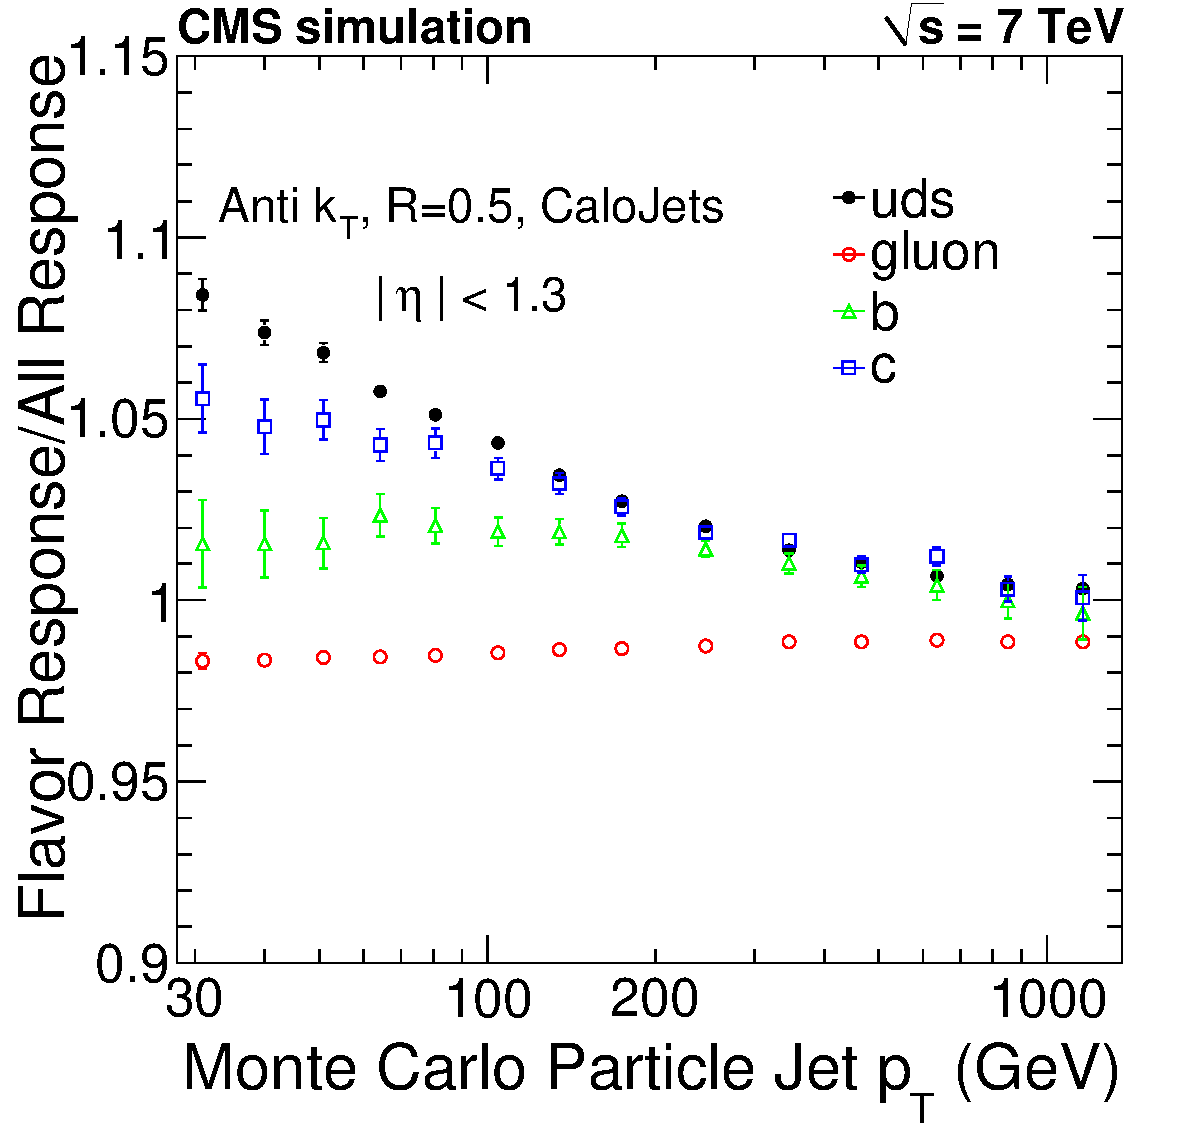
\includegraphics[width=0.32\textwidth]{Figures/JEC/ak5calo_FlavorRsp}
    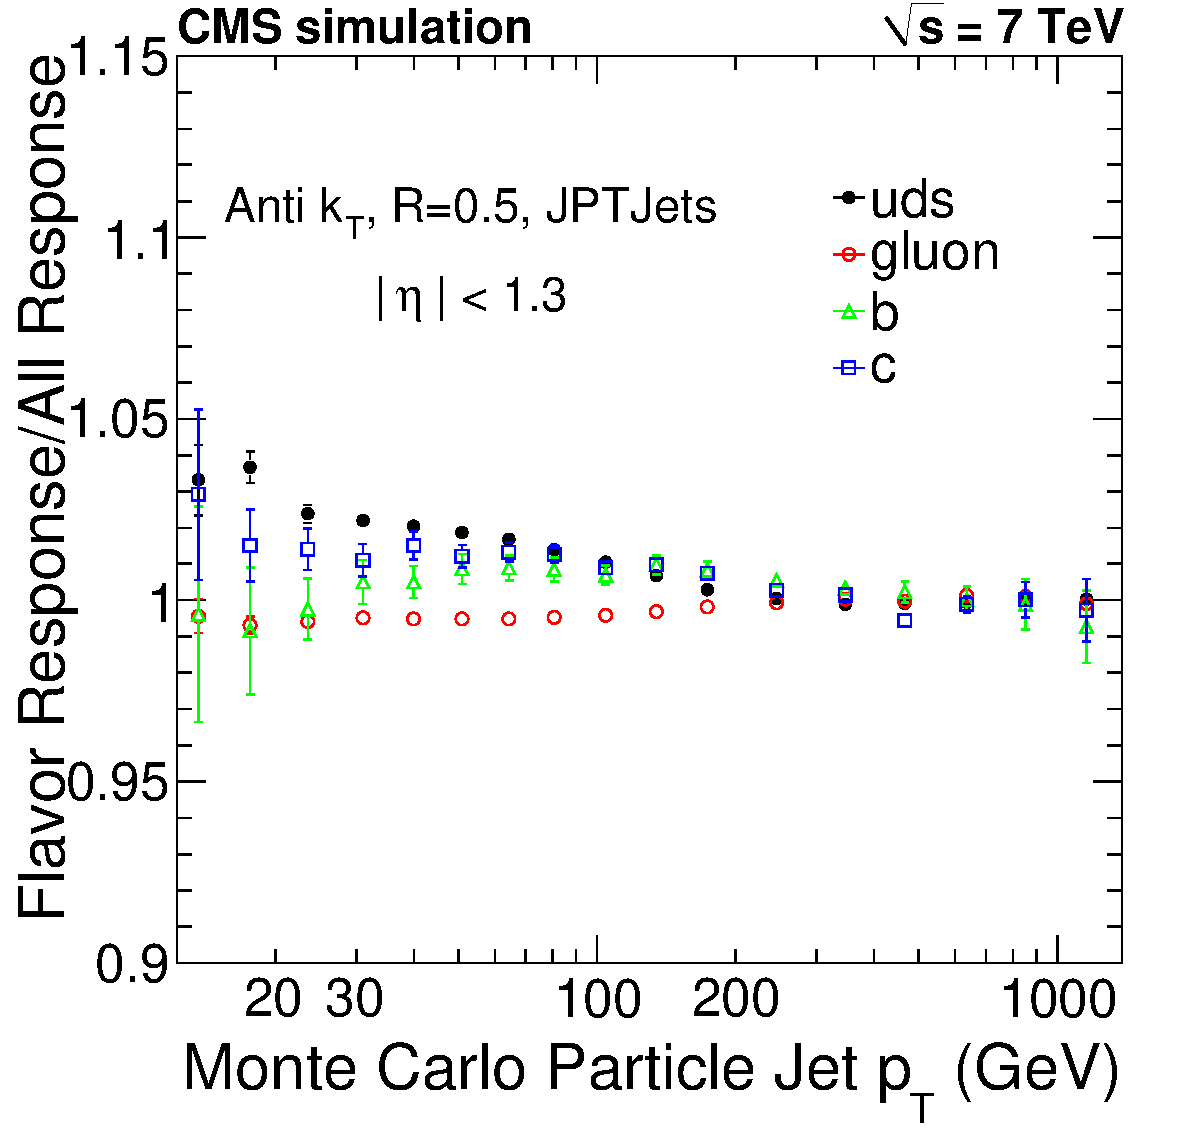
\includegraphics[width=0.32\textwidth]{Figures/JEC/ak5jpt_FlavorRsp}
    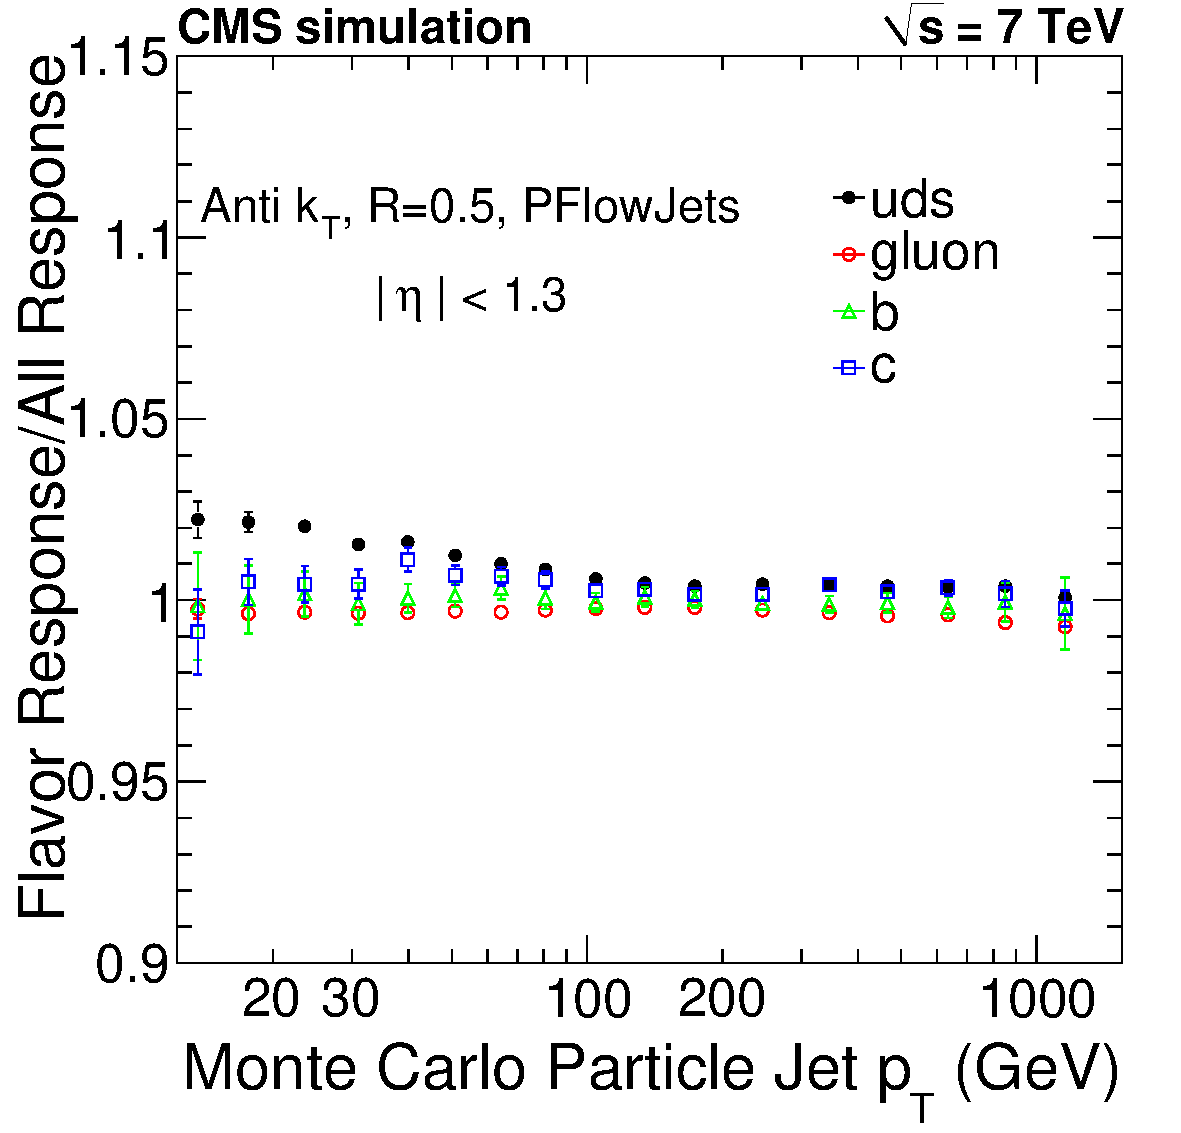
\includegraphics[width=0.32\textwidth]{Figures/JEC/ak5pf_FlavorRsp}
    \caption{Simulated jet energy response, in {\sc PYTHIA6} Z2 tune, of different jet flavours normalized to the response of the QCD flavour mixture, as a function of the true particle jet \pt, in the region $|\eta|<1.3$ for the three jet types.}
    \label{fig:flavor}
  \end{center}
\end{figure}

\begin{figure}[ht!]
  \begin{center}
    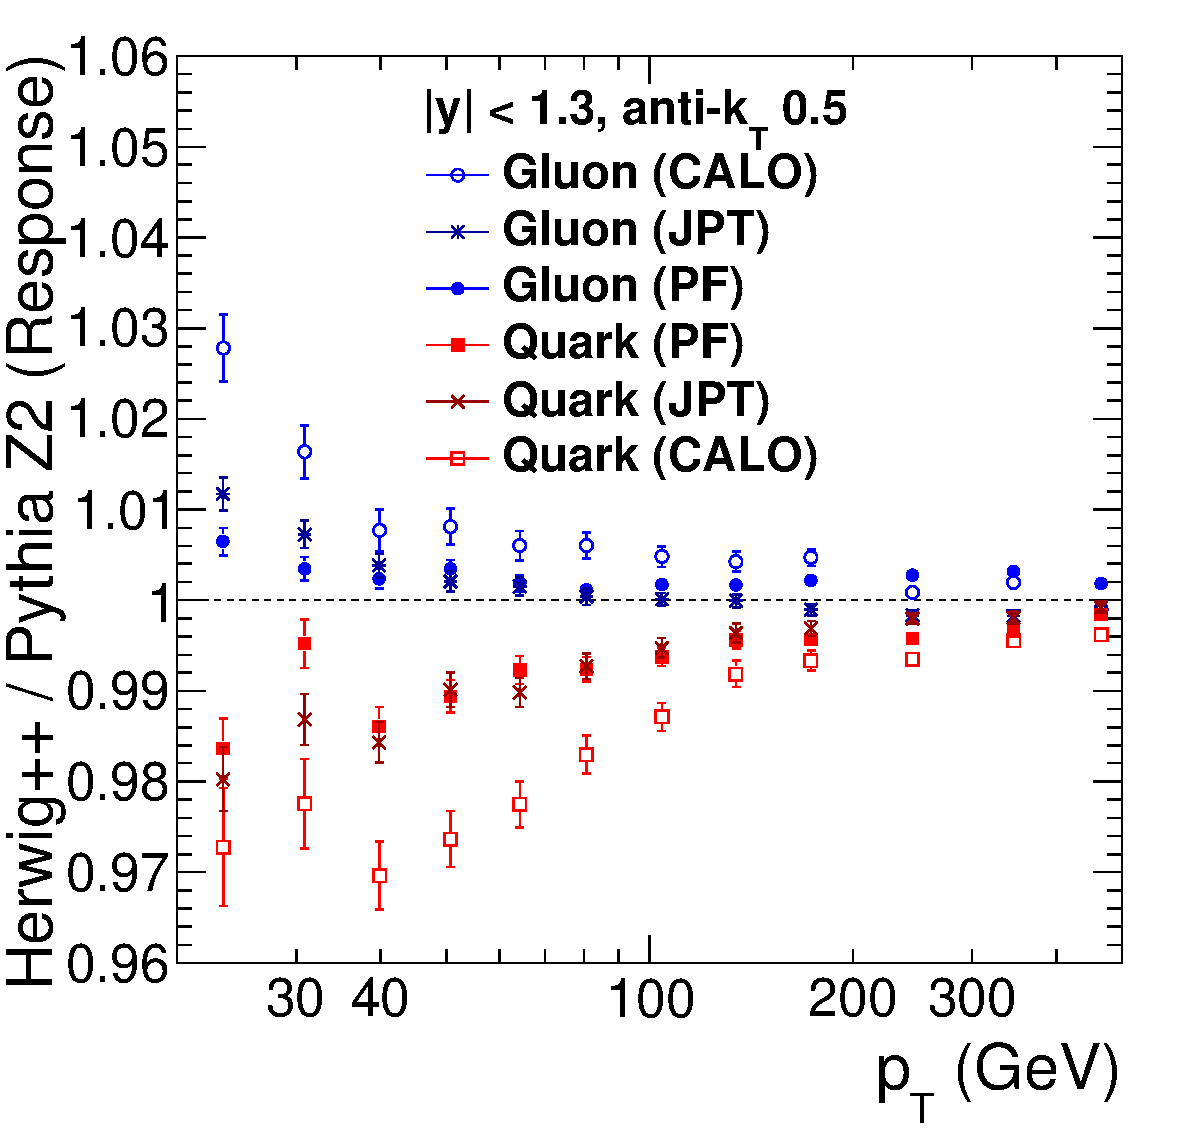
\includegraphics[width=0.45\textwidth]{Figures/JEC/flavor_herwigpythia}
    \caption{Response ratio predicted by {\sc Herwig++} and {\sc PYTHIA6} for jets originated by light quarks (uds) and gluons for the various jet types.}
    \label{fig:flavor_herwigpythia}
  \end{center}
\end{figure}

\subsection{Relative Jet Energy Scale}

\subsubsection{Measurement} 

The dijet \pt-balance technique, described in Section~\ref{sec:methods}, is used to measure the response of a jet at any $\eta$ relative to the jet energy response in the region $|\eta|<1.3$. Figure~\ref{fig:balance} shows example distributions of the balance quantity $\mathcal{B}$ for PF jets in two pseudorapidity bins. Figure~\ref{fig:relrsp} shows the relative response as a function of $\eta$ in the range $100\GeV < \ptave < 130\GeV$. Ideally, the relative response of the corrected jets in the simulation should be equal to unity. However, because of the resolution bias effect (Section~\ref{sec:resbias}), the relative response in the simulation is found to deviate from unity by an amount equal to the resolution bias. The comparison of the data with the MC simulations implicitly assumes that the resolution bias in the data is the same as in the simulation. This assumption is the dominant systematic uncertainty related to the measurement of the relative response with the dijet balance method.

\begin{figure}[ht!]
  \begin{center}
    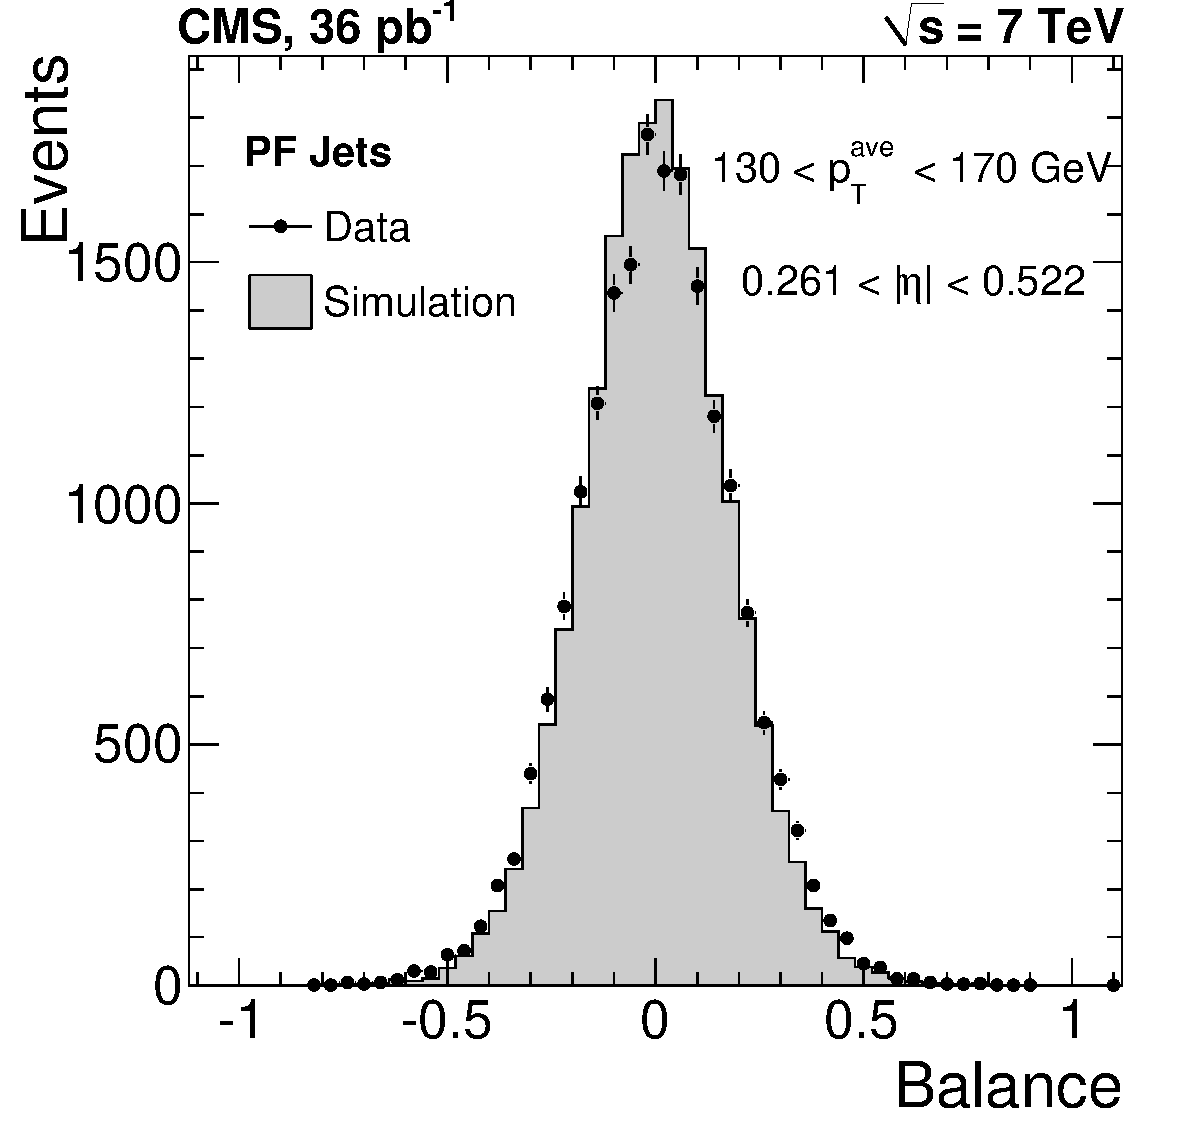
\includegraphics[width=0.45\textwidth]{Figures/JEC/B_DijetPt4_Eta1_ak5pfl1l2l3}
    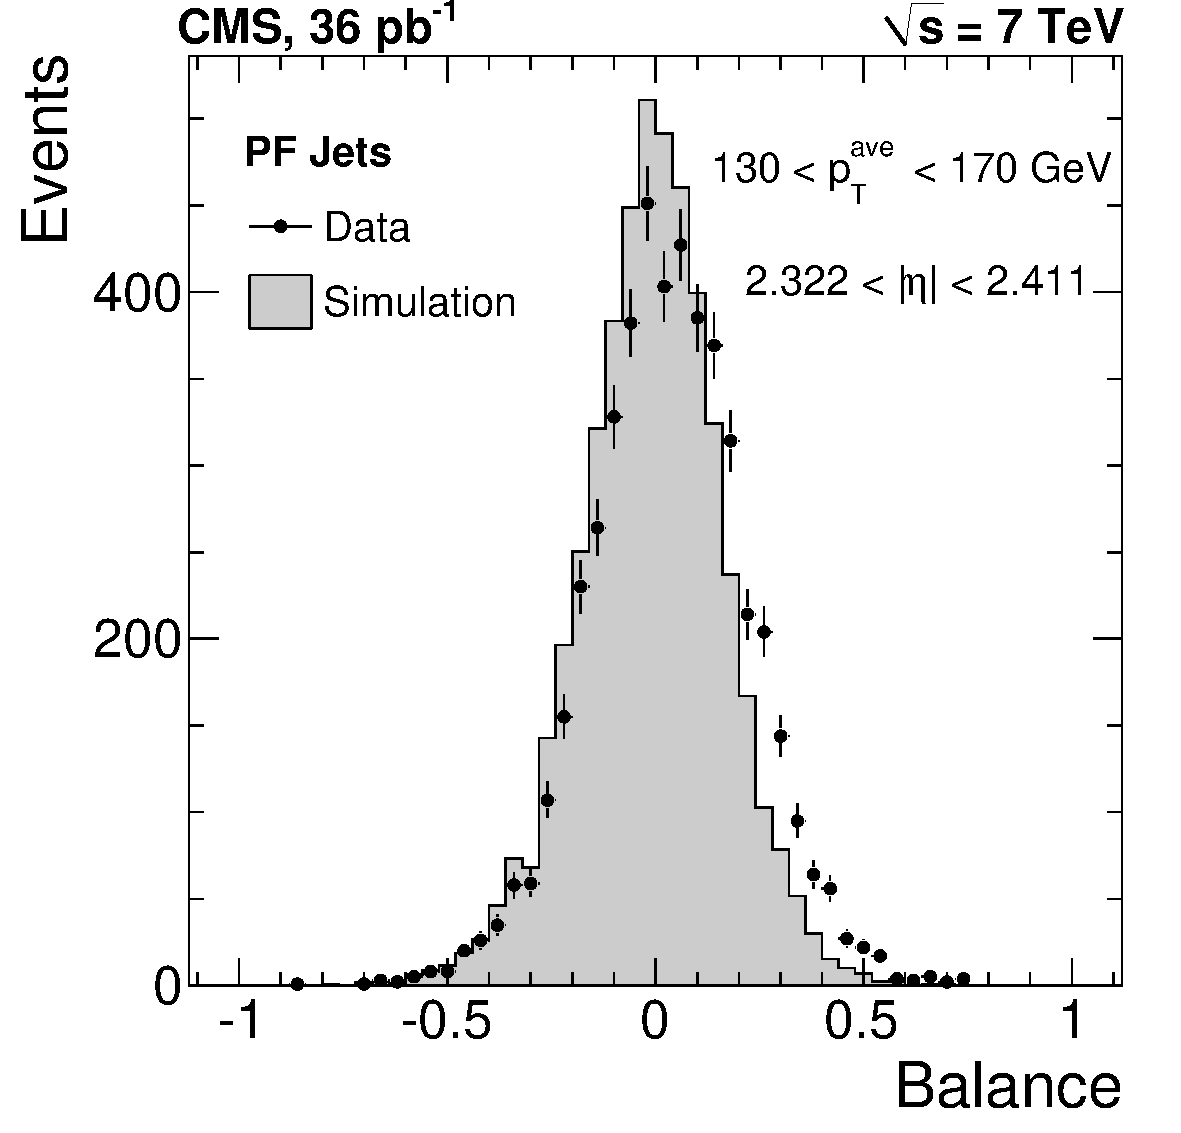
\includegraphics[width=0.45\textwidth]{Figures/JEC/B_DijetPt4_Eta9_ak5pfl1l2l3}
    \caption{Example distributions of the dijet balance quantity for PF jets in two $\eta$ regions.}
    \label{fig:balance}
  \end{center}
\end{figure}

\begin{figure}[ht!]
  \begin{center}
    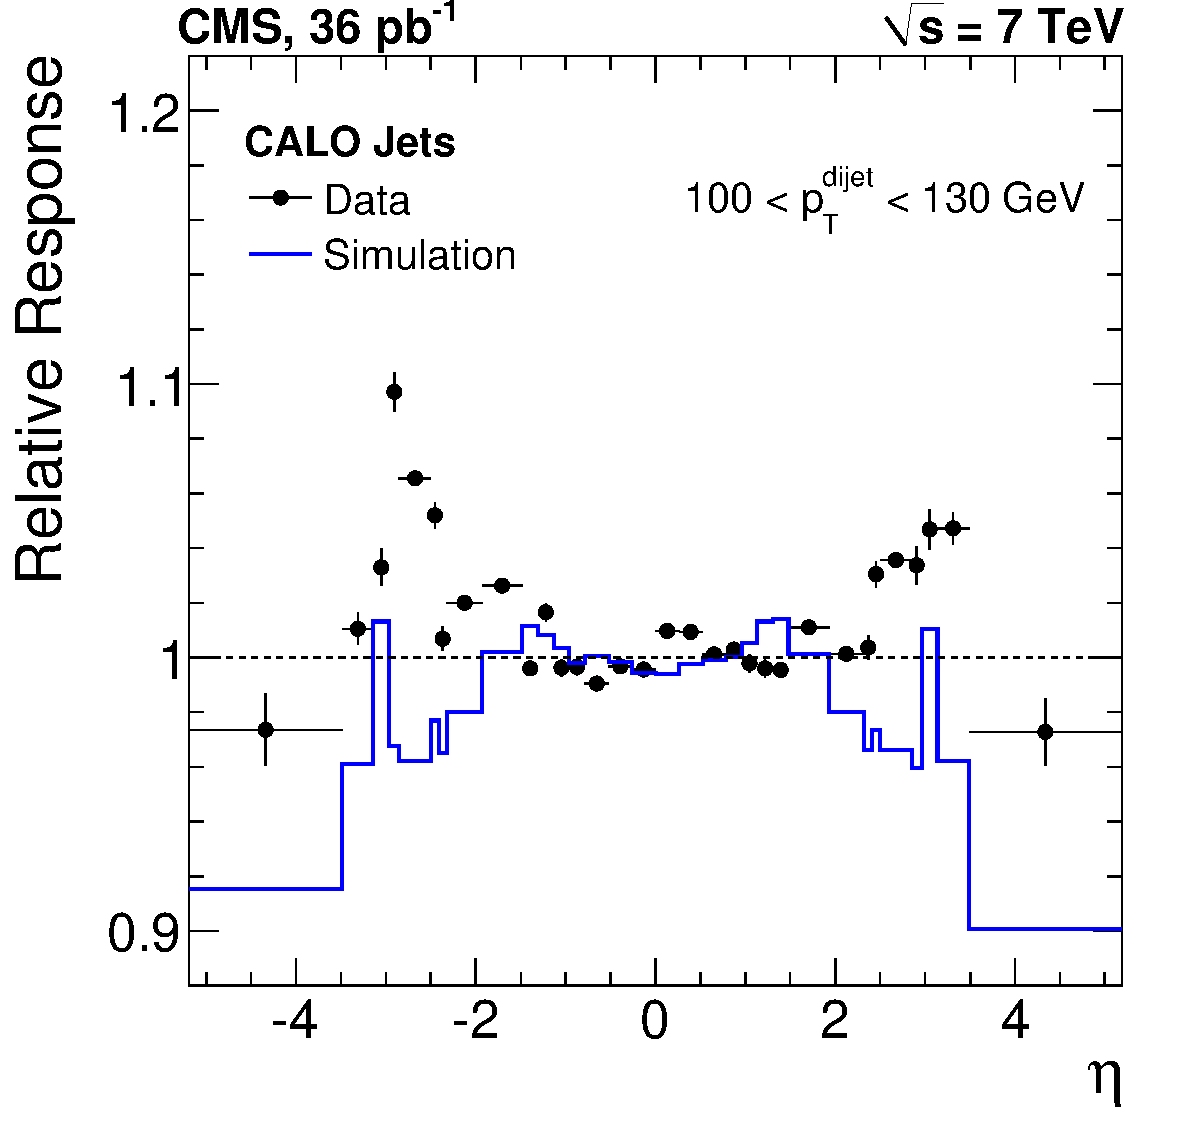
\includegraphics[width=0.45\textwidth]{Figures/JEC/RelativeResponse_Pt3_ak5calol1l2l3}
    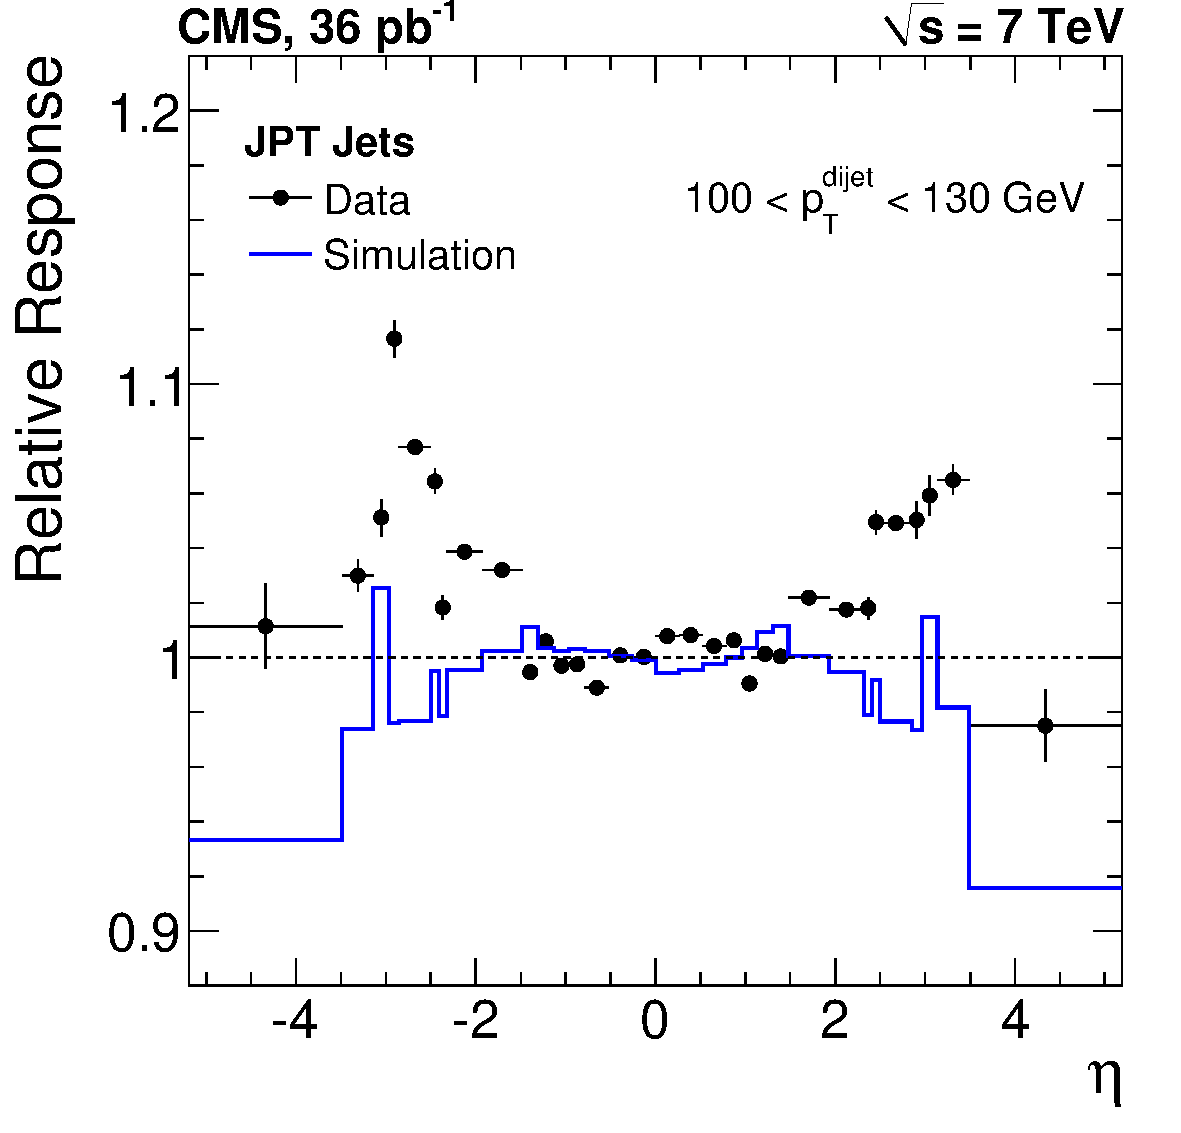
\includegraphics[width=0.45\textwidth]{Figures/JEC/RelativeResponse_Pt3_ak5jptl1l2l3}
    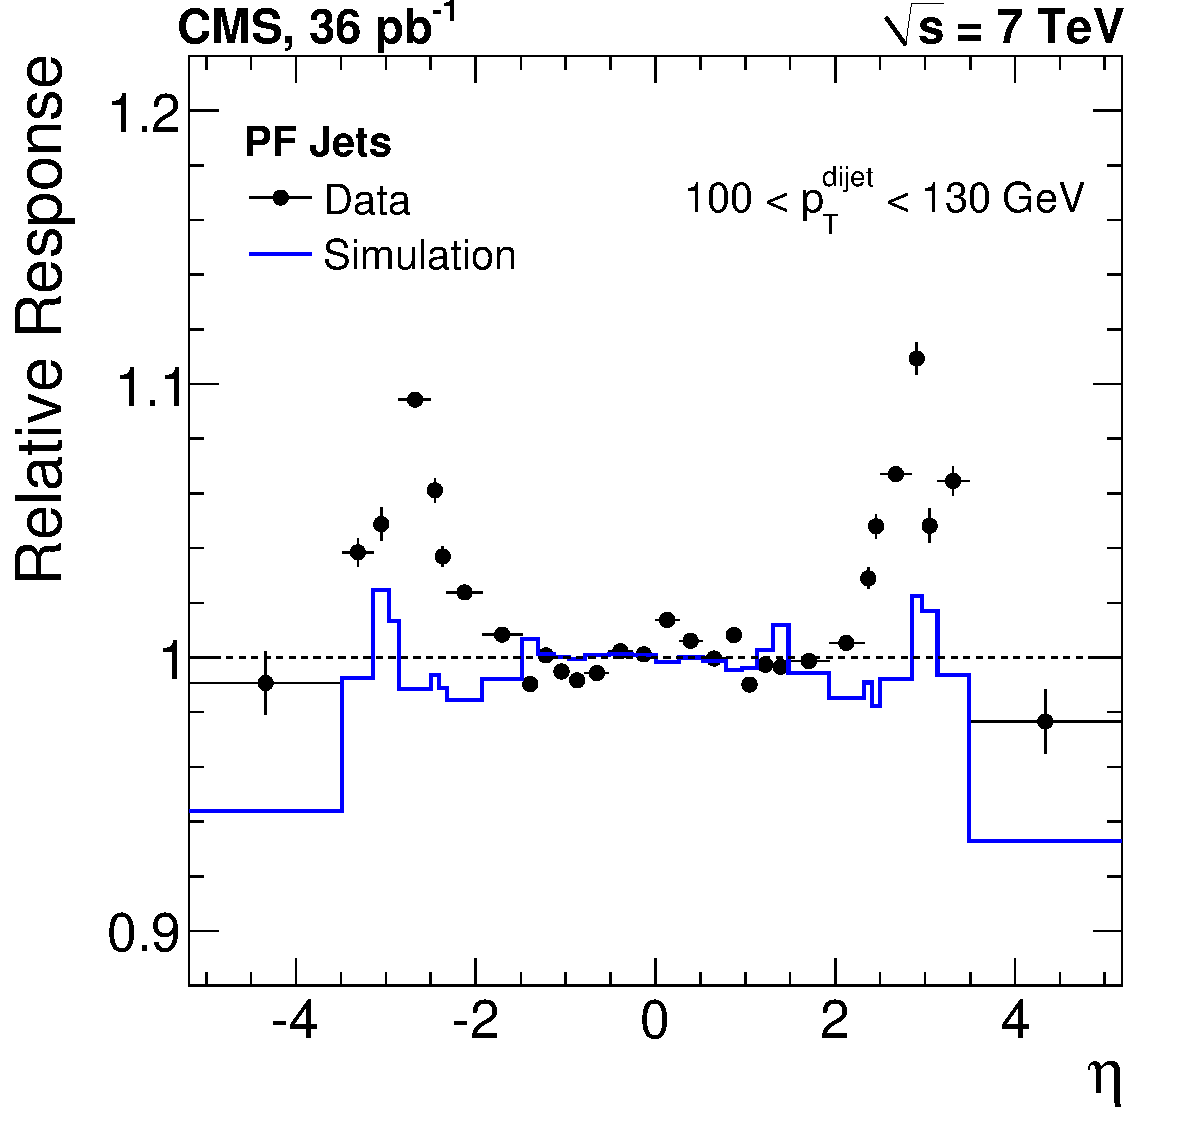
\includegraphics[width=0.45\textwidth]{Figures/JEC/RelativeResponse_Pt3_ak5pfl1l2l3}
    \caption{Relative jet energy response as a function of $\eta$, measured with the dijet balance method for CALO, JPT and PF jets respectively.}
    \label{fig:relrsp}
  \end{center}
\end{figure}

In order to reduce the radiation bias (Section~\ref{sec:radbias}), a selection is applied on the ratio $\alpha=\ptthird/\ptave$ and the nominal analysis value is $\alpha<0.2$. The residual relative correction calculation is done in three steps: first, the $\eta$-symmetric part, $C_\text{sym}$, is measured in bins of $|\eta|$, in order to maximize the available statistics, with the nominal requirement $\alpha<0.2$. Then, a correction factor $k_\text{rad}$ is applied to take care of the extrapolation to $\alpha=0$, and finally the asymmetry in $\eta$, $\mathcal{A}_R(|\eta|)$, is taken into account. The residual correction for the relative jet energy scale is formally expressed below:

\begin{equation}
  C_\text{rel}(\pm\eta) = \frac{k_\text{rad}(|\eta|)\cdot C_\text{sym}(|\eta|)}{1\mp \mathcal{A}_R(|\eta|)}.
\end{equation}

The $C_\text{sym}$ component is defined by comparing the relative response in data and MC simulations: 

\begin{equation}
  C_\text{sym}(|\eta|) = \left<\frac{R_{MC}^{\alpha<0.2}}{R_{data}^{\alpha<0.2}}\right>_{\pt},
\end{equation}

averaged over the entire \pt range. This is justified by the fact that no statistically significant \pt-dependence is observed in the comparison between data and simulation.

Since the additional radiation and the UE are not perfectly modeled in the simulation, a correction needs to be applied by extrapolating to zero third-jet activity, as discussed in Section~\ref{sec:radbias}. The radiation correction $k_{rad}$ is defined as: 

\begin{equation}
  k_\text{rad} = \lim_{\alpha\to 0}\left(\dfrac{\left<\frac{R_{MC}^\alpha}{R_{data}^\alpha}\right>_{\pt}}{\left<\frac{R_{MC}^{\alpha<0.2}}{R_{data}^{\alpha<0.2}}\right>_{\pt}}\right).
\end{equation}

Figure~\ref{fig:FSR} (left) shows the radiation correction that needs to be applied to the measurement at the working point $\alpha<0.2$. The correction is negligible in the central region while it reaches the value of 3\% at larger rapidities.

\begin{figure}[ht!]
  \begin{center}
    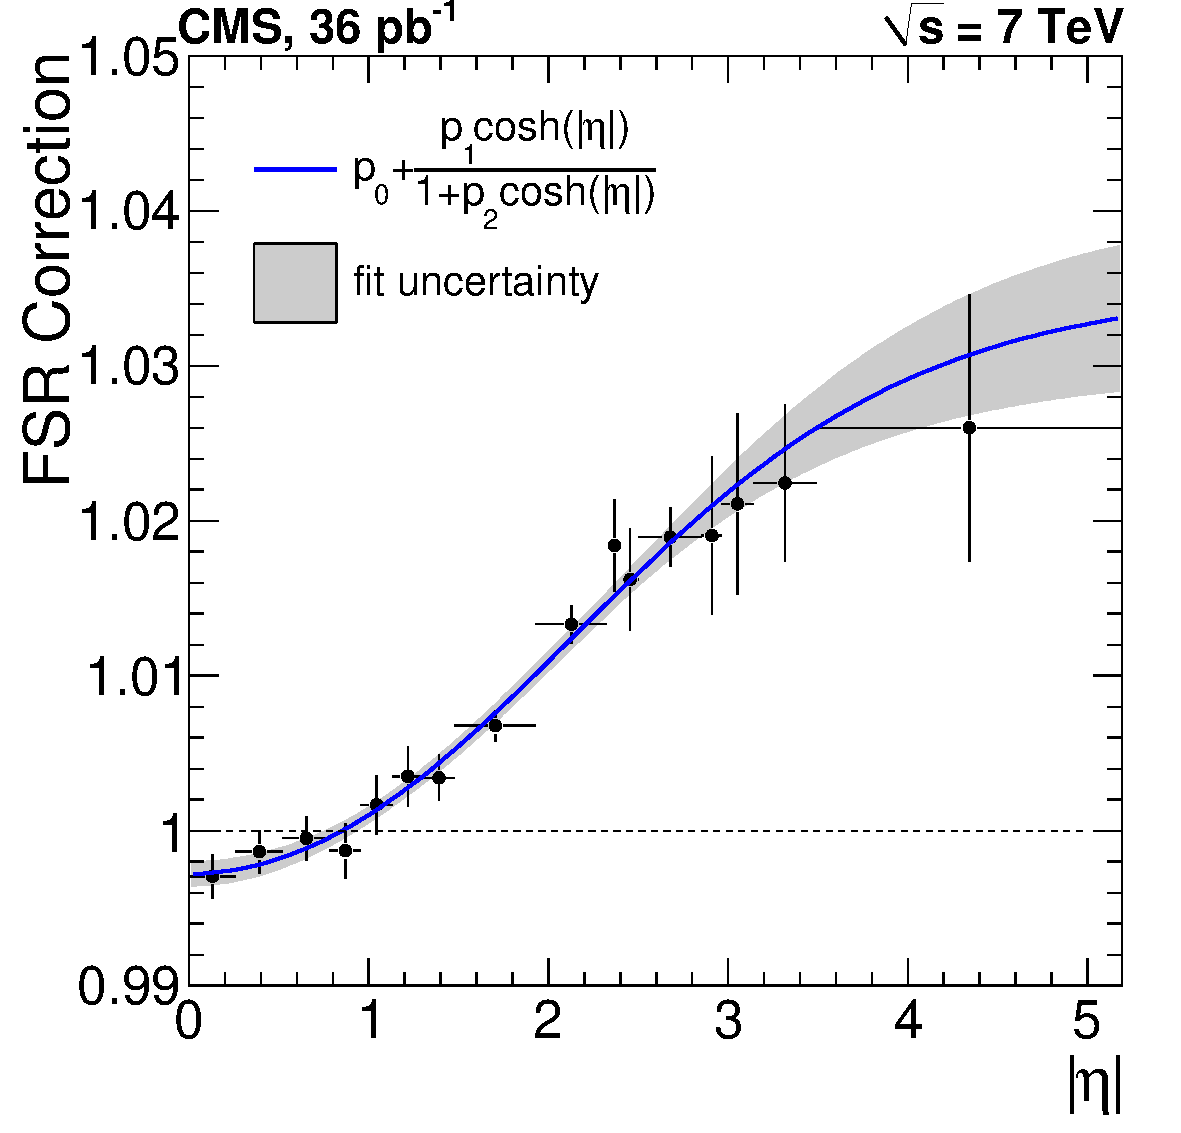
\includegraphics[width=0.45\textwidth]{Figures/JEC/FSR}
    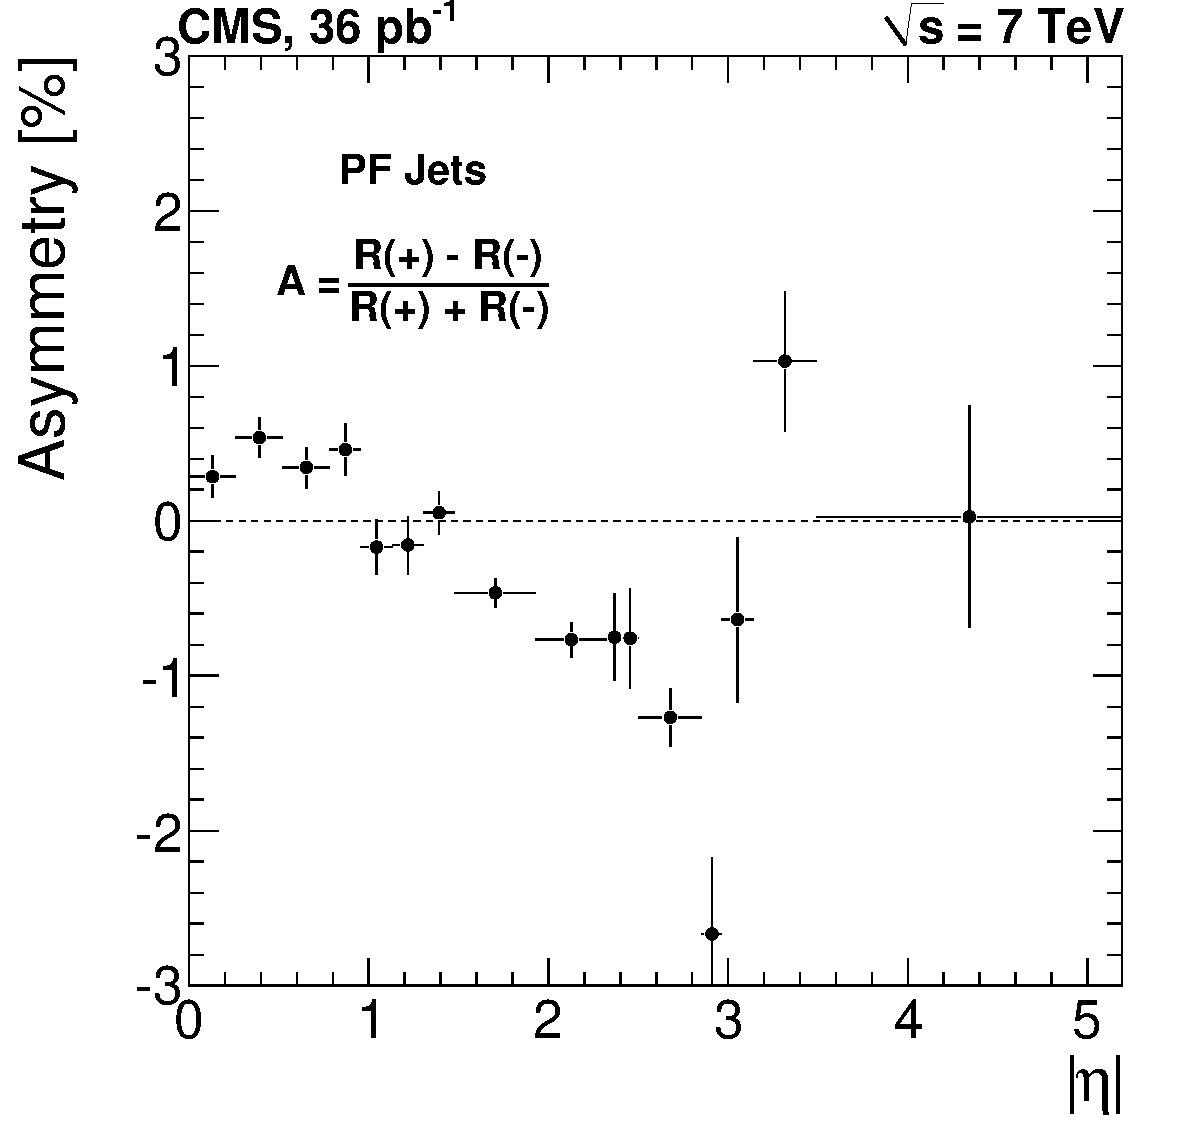
\includegraphics[width=0.45\textwidth]{Figures/JEC/AsymmetryVsEta_ak5pfl1l2l3}
    \caption{Left: correction $k_\text{rad}$ of the relative jet energy residual due to initial and final state radiation. Right: relative jet energy response asymmetry as a function of jet $|\eta|$, for $\alpha<0.2$.}
    \label{fig:FSR}
  \end{center}
\end{figure}

The asymmetry of the response in $\eta$ is quantified through the variable $\mathcal{A}_R$:

\begin{equation}
  \mathcal{A}_R(|\eta|) = \frac{R(+|\eta|)-R(-|\eta|)}{R(+|\eta|)+R(-|\eta|)},
\end{equation}

where $R(+|\eta|)$ ($R(-|\eta|)$) is the relative response measured in the data at the detector part lying in the direction of the positive (negative) z-axis. Figure~\ref{fig:FSR} (right) shows the measured asymmetry. It is found to be similar for the different jet types.

Figure~\ref{fig:final_residual} shows the final residual correction, as a function of $\eta$, for all jet types. This correction is typically of the order of 2-3\%, with the exception of the region $2.5<|\eta|<3.0$ where it reaches the value of 10\%. The region where the larger discrepancy between data and MC simulations is observed (Fig.~\ref{fig:relrsp}), coincides with the border between the endcap and the forward calorimeters. It has also been observed~\cite{JME-10-008} that the single-particle response shows similar behavior in this region.

\begin{figure}[ht!]
  \begin{center}
    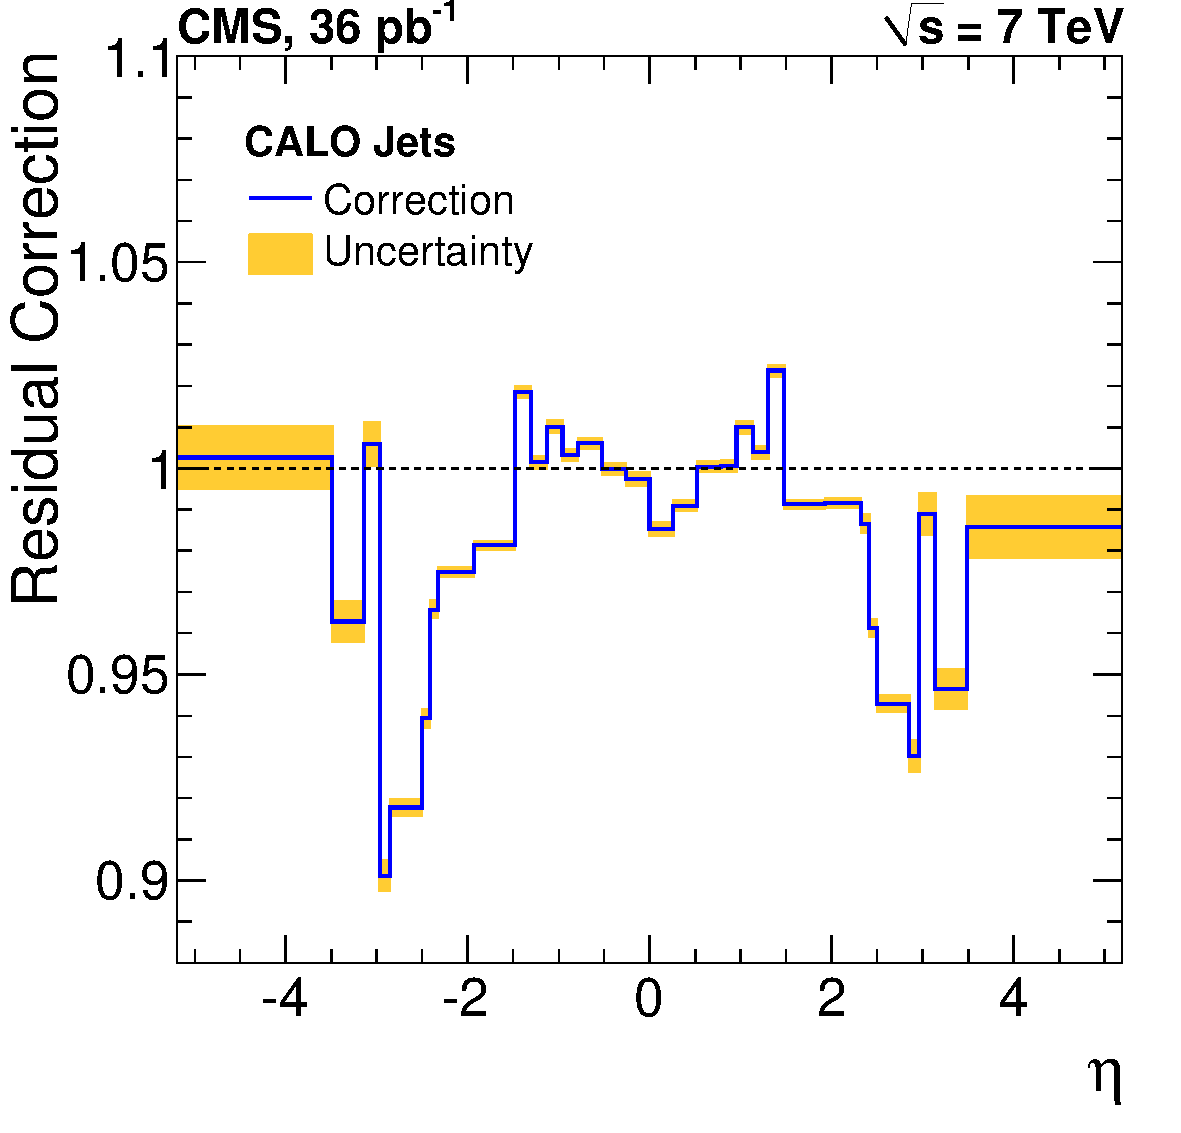
\includegraphics[width=0.45\textwidth]{Figures/JEC/FinalResidual_ak5calol1l2l3}
    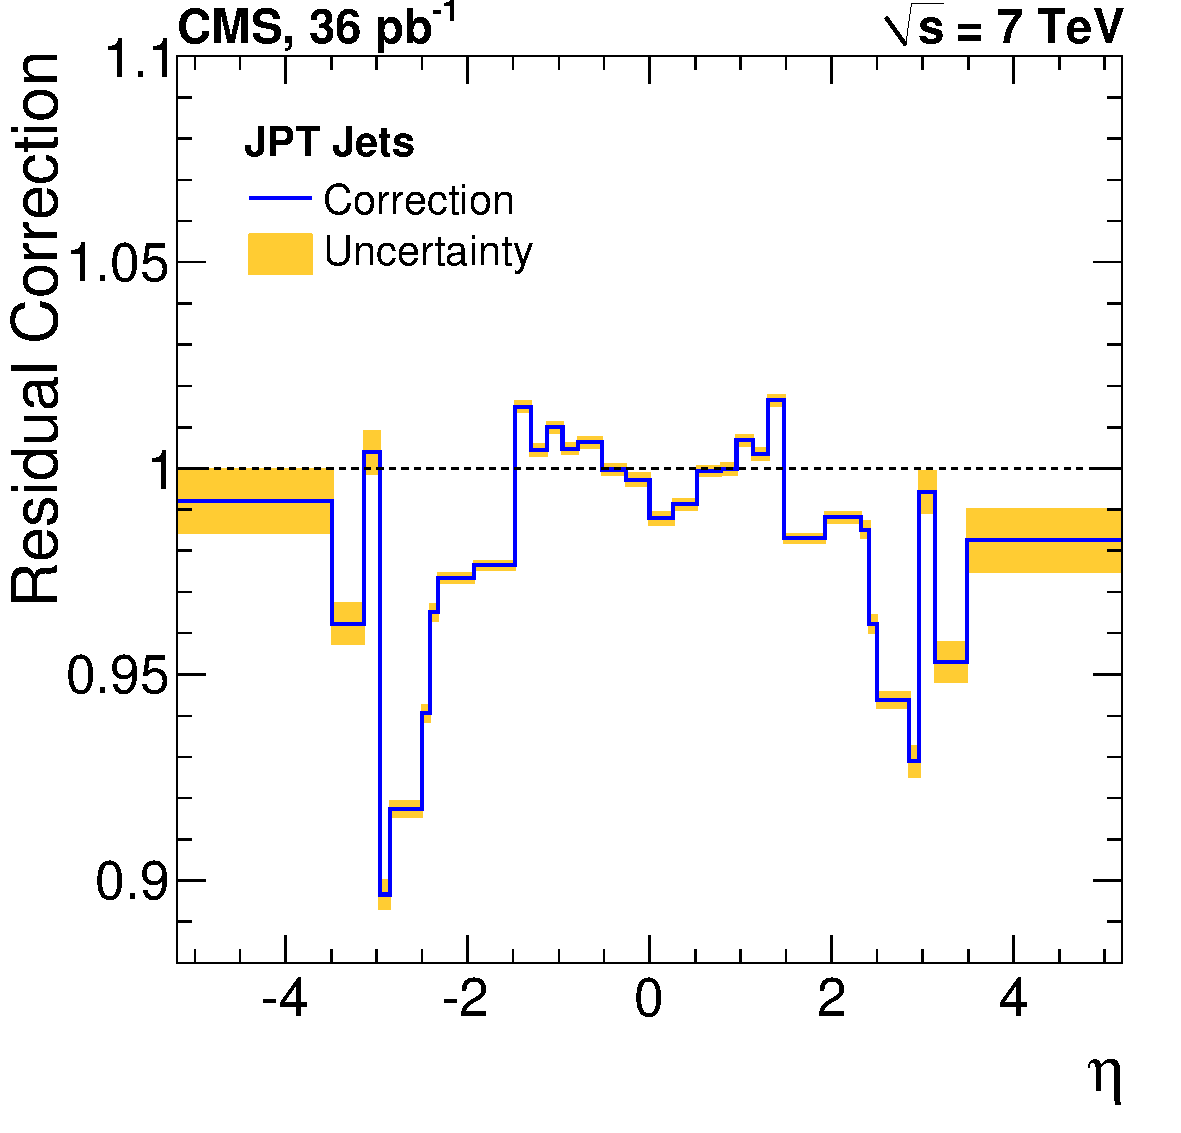
\includegraphics[width=0.45\textwidth]{Figures/JEC/FinalResidual_ak5jptl1l2l3}
    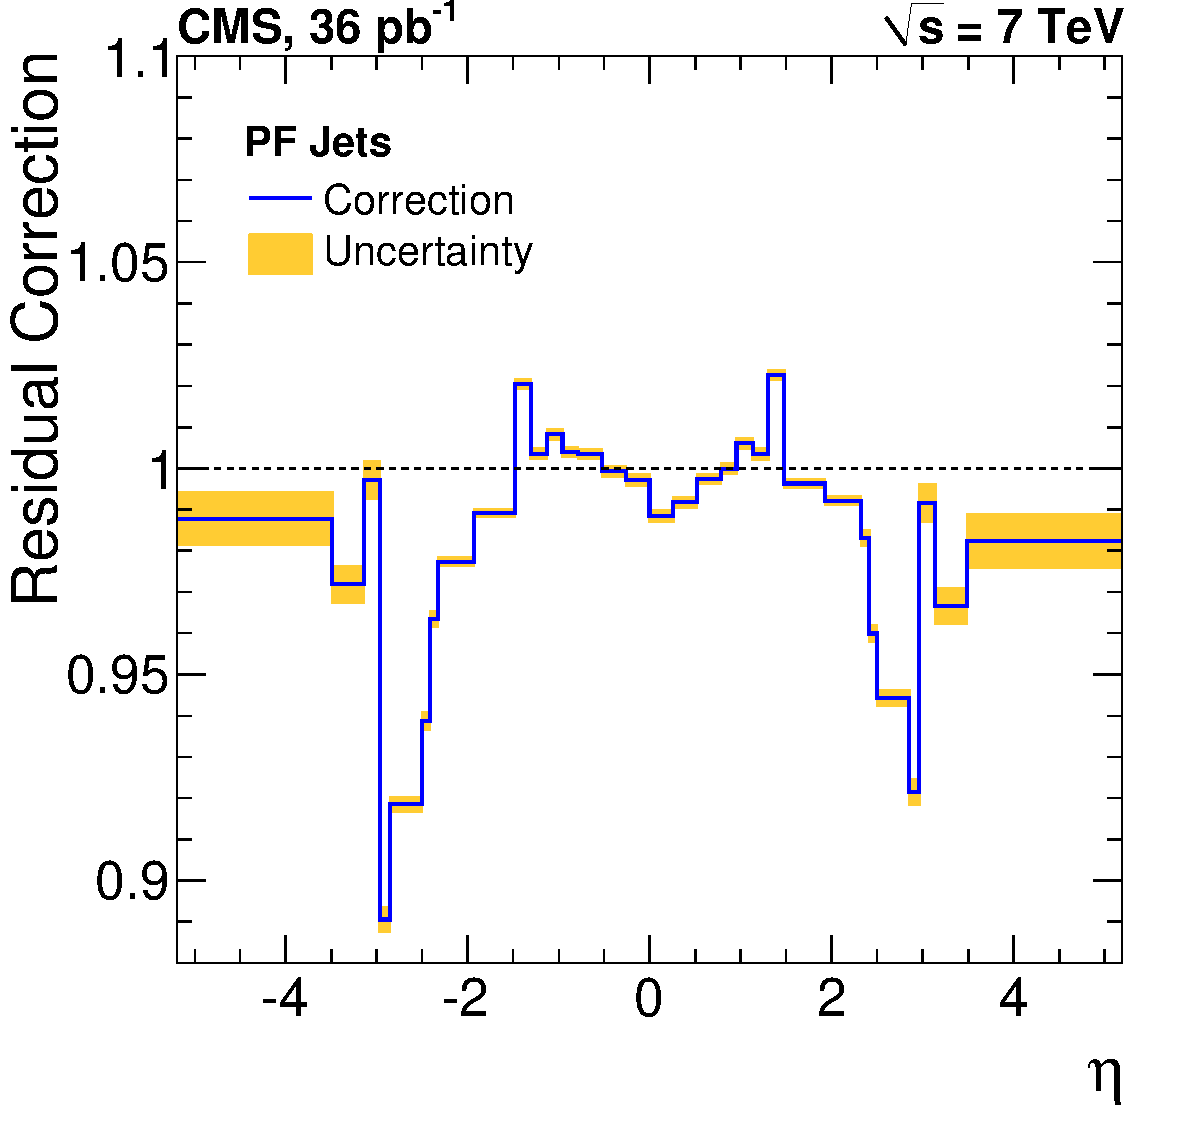
\includegraphics[width=0.45\textwidth]{Figures/JEC/FinalResidual_ak5pfl1l2l3}
    \caption{Relative jet energy residual correction as a function of jet $\eta$ for CALO, JPT and PF jets respectively. The band shows the uncertainty due to statistics, radiation corrections, and asymmetry in $\eta$.}
    \label{fig:final_residual}
  \end{center}
\end{figure}

Finally, Fig.~\ref{fig:L2Closure} demonstrates that the derived residual correction establishes an almost perfect agreement between data and simulation.

\begin{figure}[ht!]
  \begin{center}
    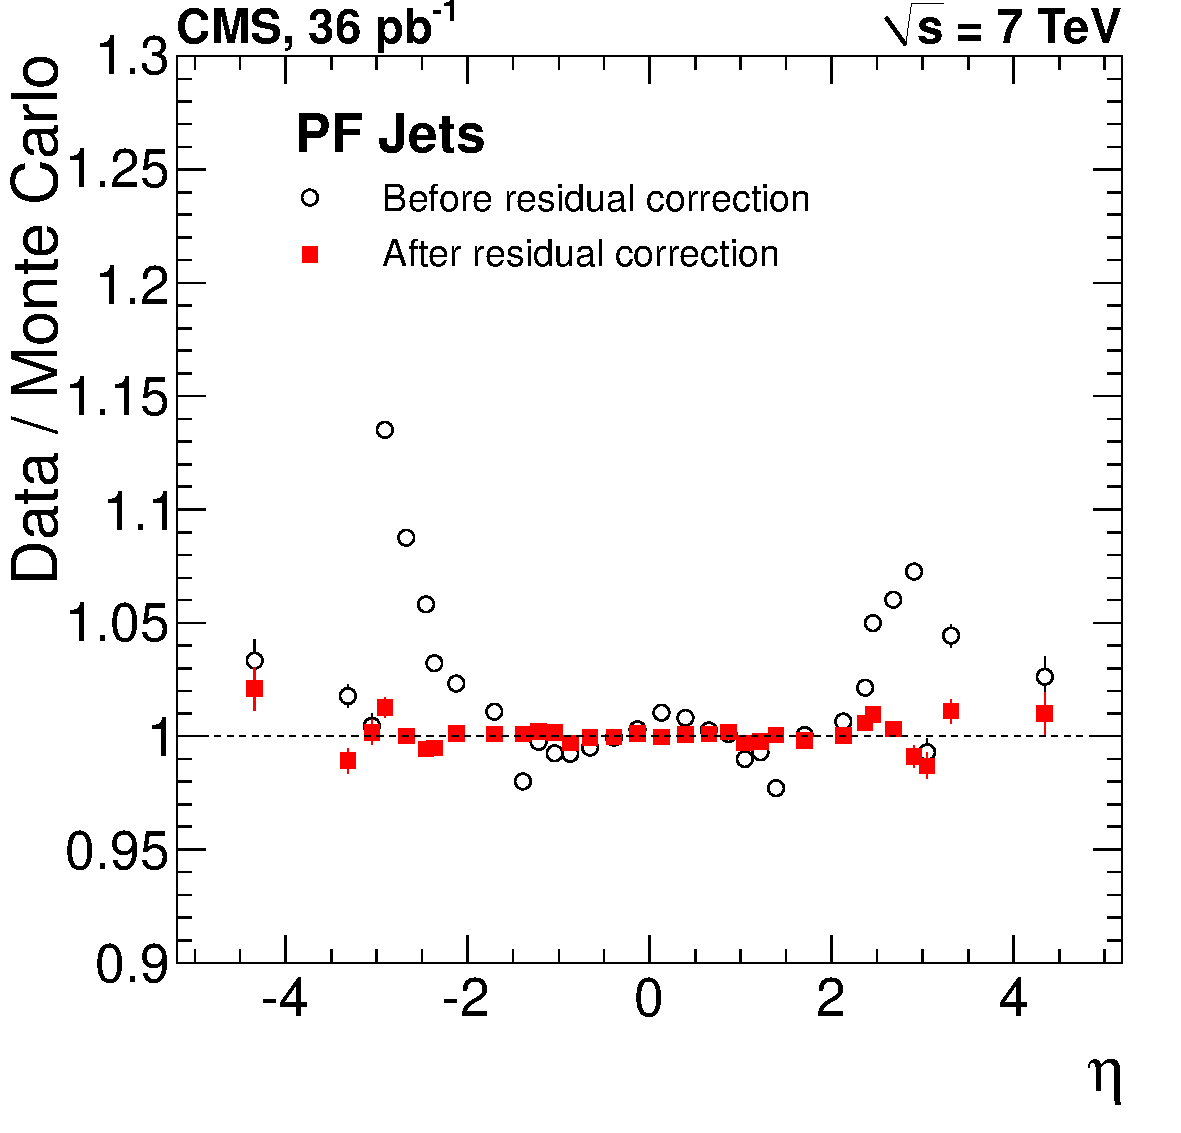
\includegraphics[width=0.45\textwidth]{Figures/JEC/RelResponseClosurePF.pdf}
    \caption{Relative response ratio between data and MC simulation before and after the residual correction.}
    \label{fig:L2Closure}
  \end{center}
\end{figure}

\subsubsection{Uncertainty}

The dominant uncertainty of the relative residual correction is due to the simulation of the jet energy resolution, which defines the magnitude of the resolution bias. The estimate of the systematic uncertainty is achieved by varying the jet \pt resolution according to the comparisons between data and MC simulations shown in Section~\ref{sec:res}. Other sources of uncertainty, such as lack of available events, radiation correction and asymmetry in $\eta$ are found to be smaller than 1\%. The total uncertainty of the relative jet energy scale is shown in Fig.~\ref{fig:residual_unc} as a function of the jet $|\eta|$ for two characteristic values of jet \pt (50\GeV, 200\GeV). The CALO jets have systematically larger uncertainty, as opposed to PF jets which have the smallest while the JPT jets uncertainty lies between the values for the other two jet types. This pattern is consistent with the behavior of the jet energy resolution. Also, it is observed that the relative scale uncertainty grows toward larger rapidities because of the larger resolution uncertainty. 

\begin{figure}[ht!]
  \begin{center}
    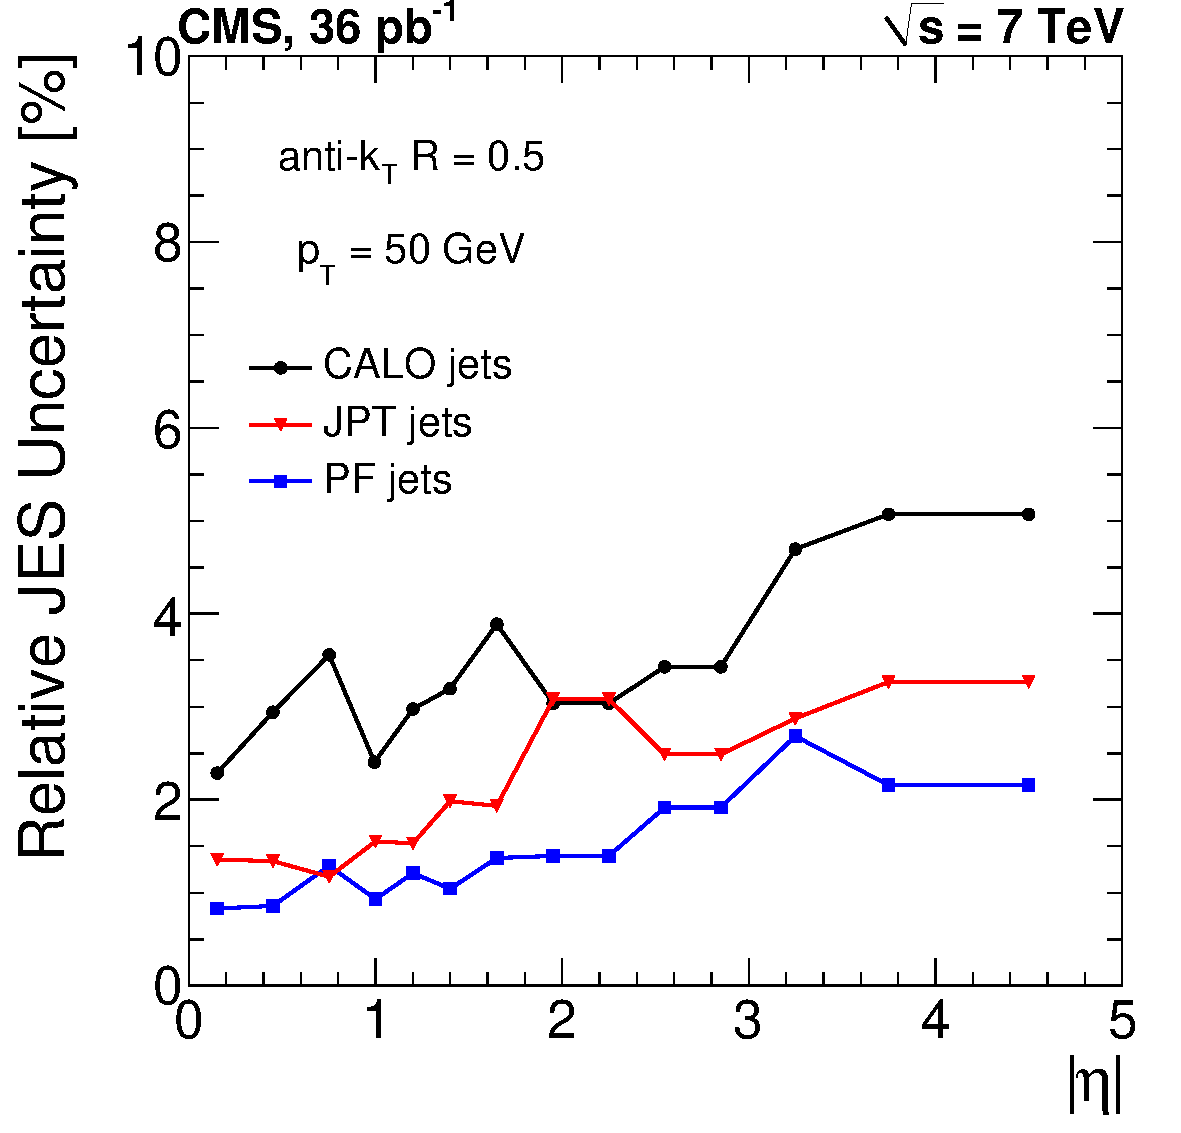
\includegraphics[width=0.45\textwidth]{Figures/JEC/ResidualUncertainty_Pt50}
    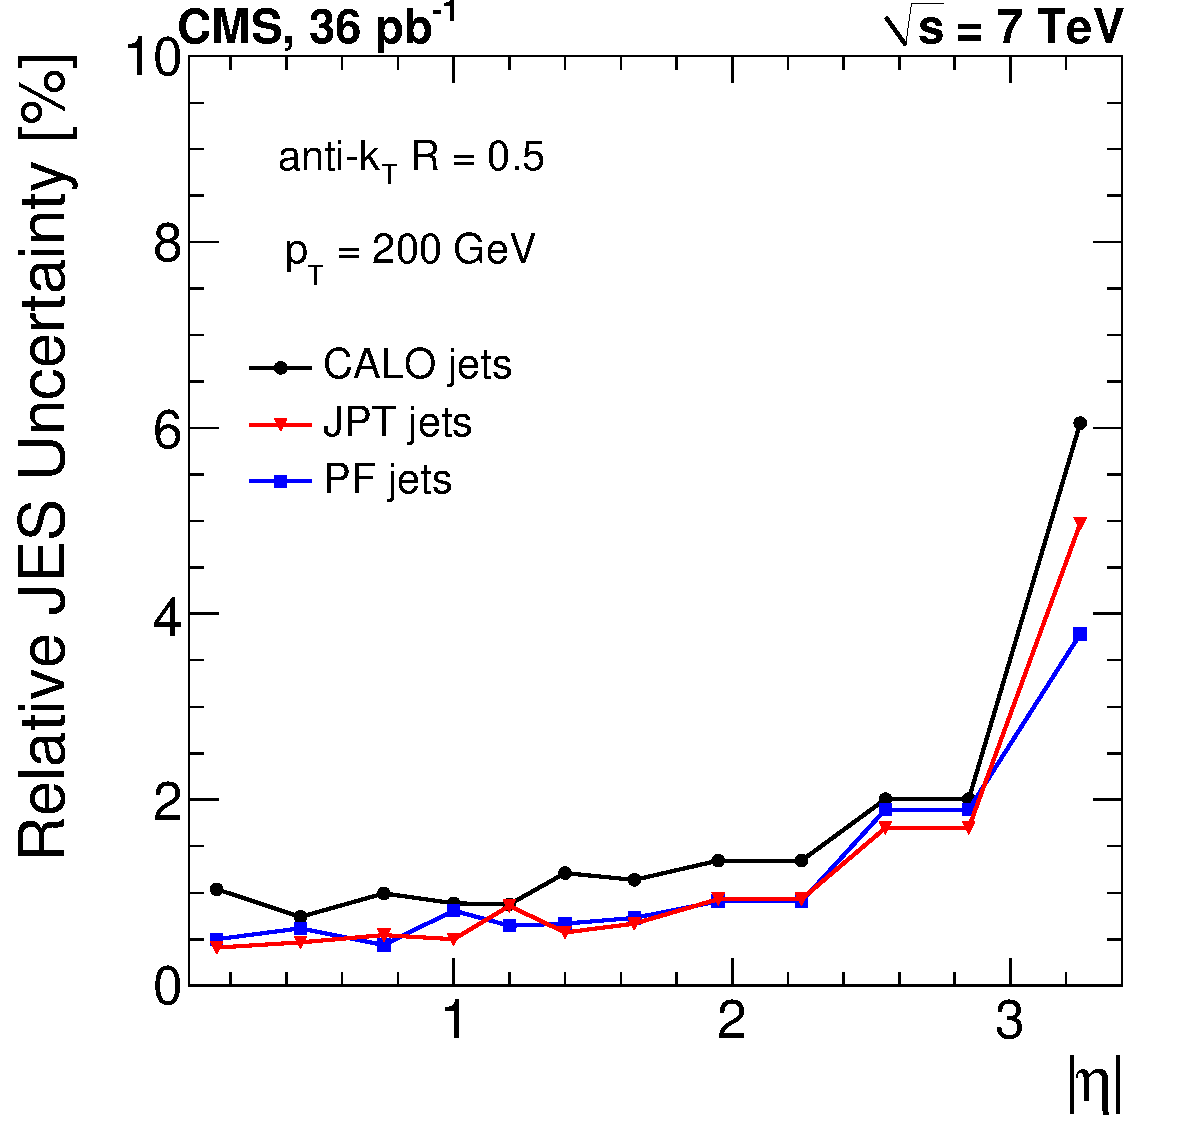
\includegraphics[width=0.45\textwidth]{Figures/JEC/ResidualUncertainty_Pt200}
    \caption{Relative jet energy residual correction uncertainty, as a function of $\eta$ for jet $\pt=50\GeV$ (left) and $\pt=200\GeV$ (right).}
    \label{fig:residual_unc}
  \end{center}
\end{figure}

\clearpage

\subsection{Absolute Jet Energy Scale}
\subsubsection{Measurement}
The absolute jet energy response is measured in the reference region $|\eta|<1.3$ with the MPF method using $\gamma/Z$+jets events,  and the result is verified with the \pt-balancing method. The $\gamma$ or the Z are used as reference objects because their energy is accurately measured in ECAL (photon, $Z\rightarrow e^+e^-$) or in the tracker and muon detectors ($Z\rightarrow \mu^+\mu^-$). Figure~\ref{fig:photonResponse} shows example distributions of the MPF and \pt-balancing methods for PF jets in the $\gamma$+jet sample.

The actual measurement is performed only for PF jets because of the full consistency between the jet and the \vecmet reconstruction (both use the same PF candidates as inputs). The absolute energy scale of the remaining jet types (CALO, PF) is determined by comparison to the corresponding PF jet after jet-by-jet matching in the $\eta-\phi$ space.    

\begin{figure}[ht!]
  \begin{center}
    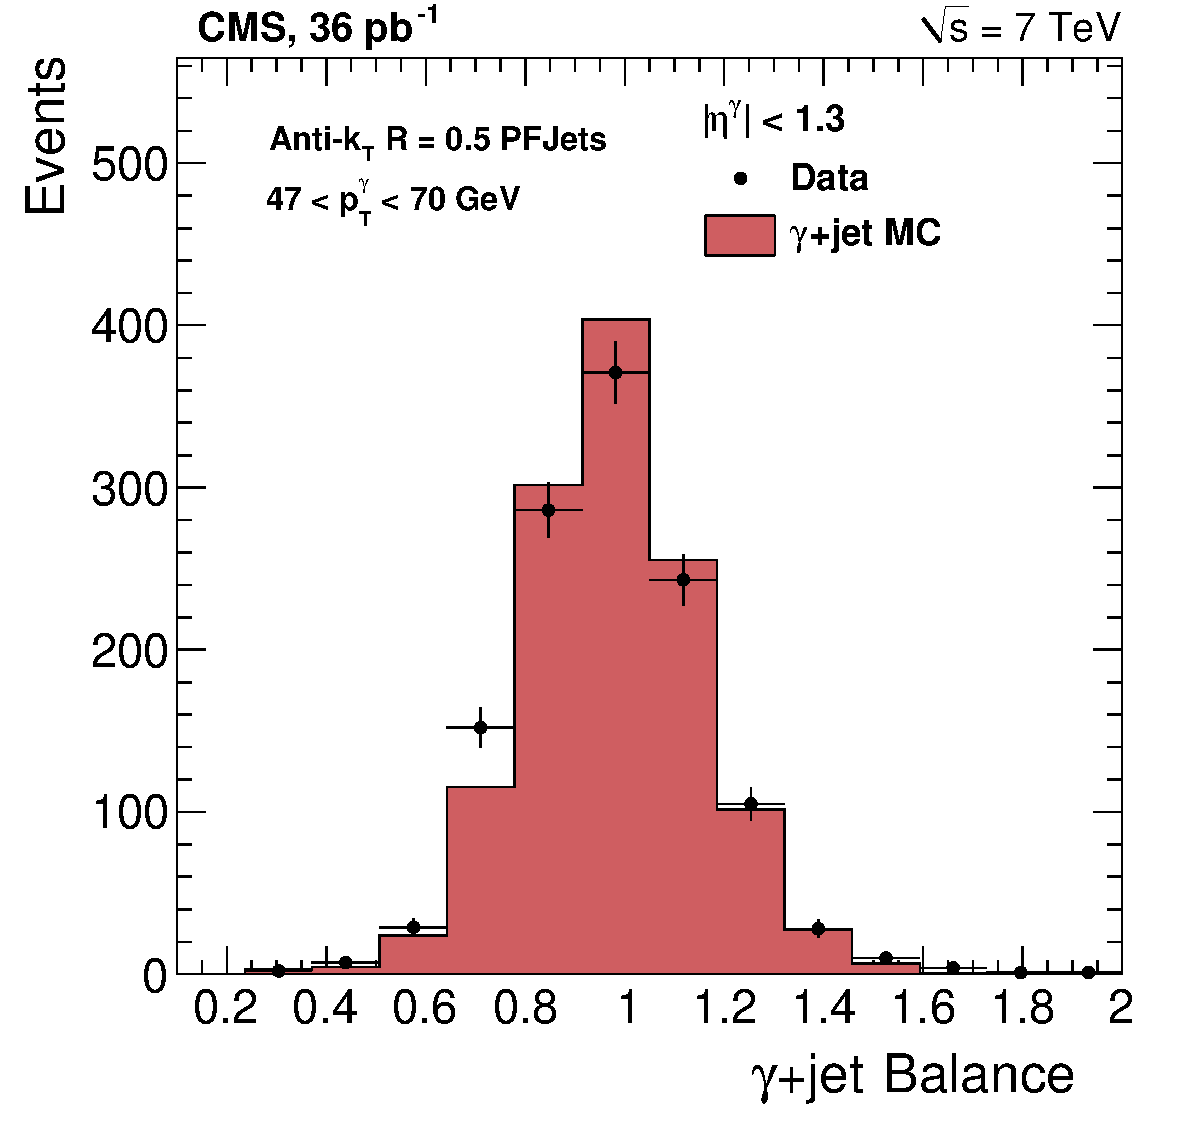
\includegraphics[width=0.45\textwidth]{Figures/JEC/response_L2L3_eta013_ptPhot_47_70}
    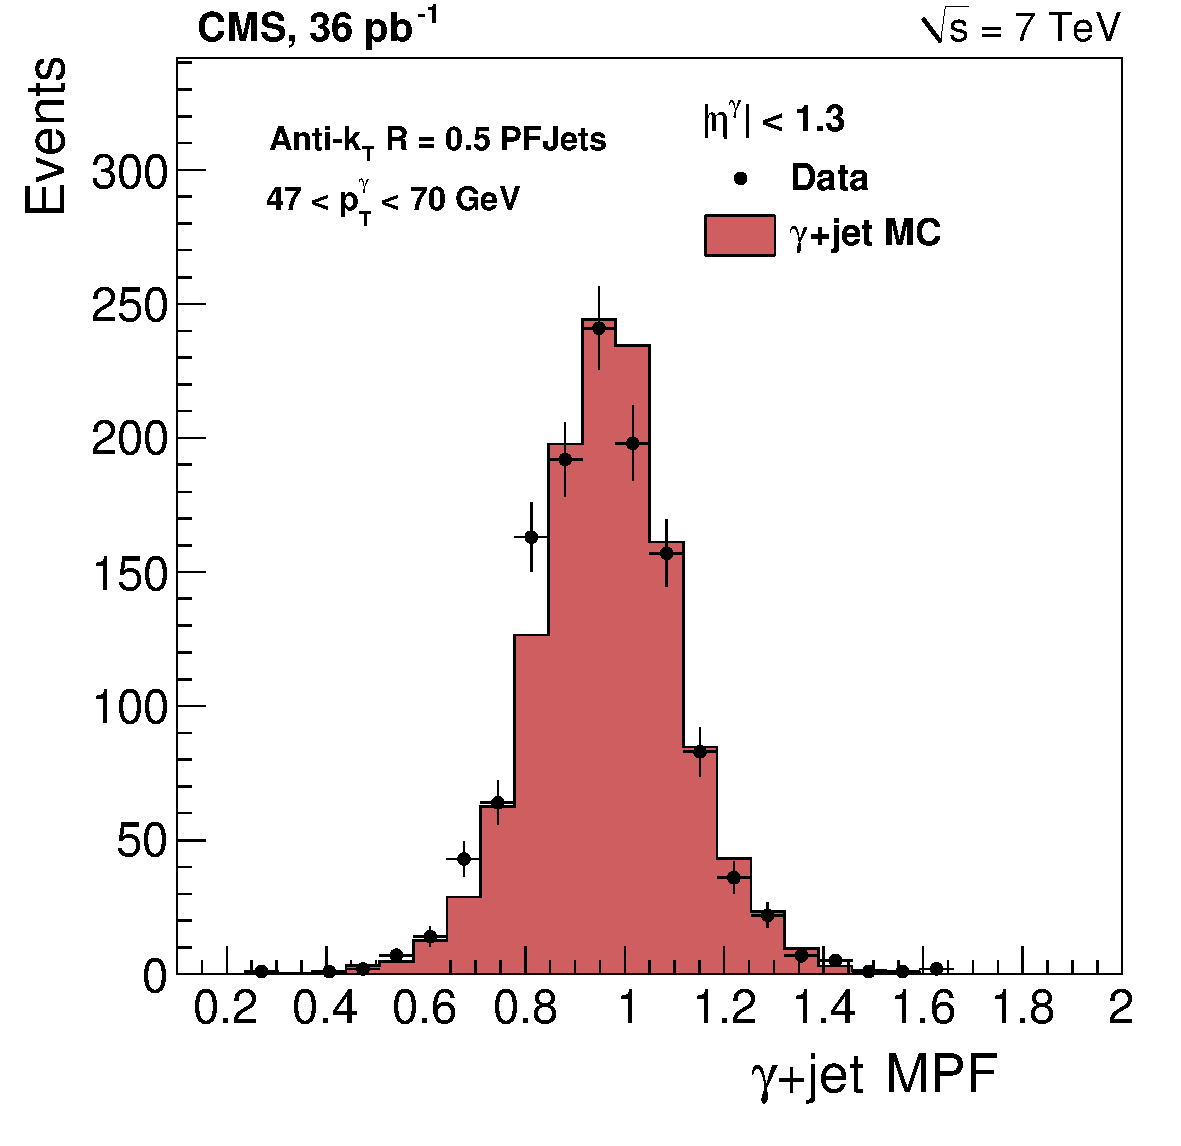
\includegraphics[width=0.45\textwidth]{Figures/JEC/responseMPF_eta013_ptPhot_47_70}
    \caption{Example response distributions for PF jets from \pt-balancing (left) and MPF (right) in the $\gamma$+jets sample.}
    \label{fig:photonResponse}
  \end{center}
\end{figure}

In the selected $\gamma$+jets sample, the presence of a barrel jet ($|\eta|<1.3$) recoiling against the photon candidate in azimuth by $\Delta \phi > 2.7$ is required. To reduce the effect of initial and final state gluon radiation that degrades the jet-photon \pt-balance, events containing additional jets with $\ptsecond > \alpha\cdot\pt^{\gamma}$ and outside the $\DeltaR=0.25$ cone around the photon direction are vetoed. The \pt-balance and MPF response measurements are performed in the same way with data and MC samples with different values of the threshold on $\alpha$ and the data/MC ratio is extrapolated to $\alpha=0$. This procedure allows the separation of the $\gamma$-jet intrinsic \pt-imbalance from the imbalance caused by hard radiation (Section~\ref{sec:radbias}). 

\begin{figure}[ht!]
  \begin{center}
    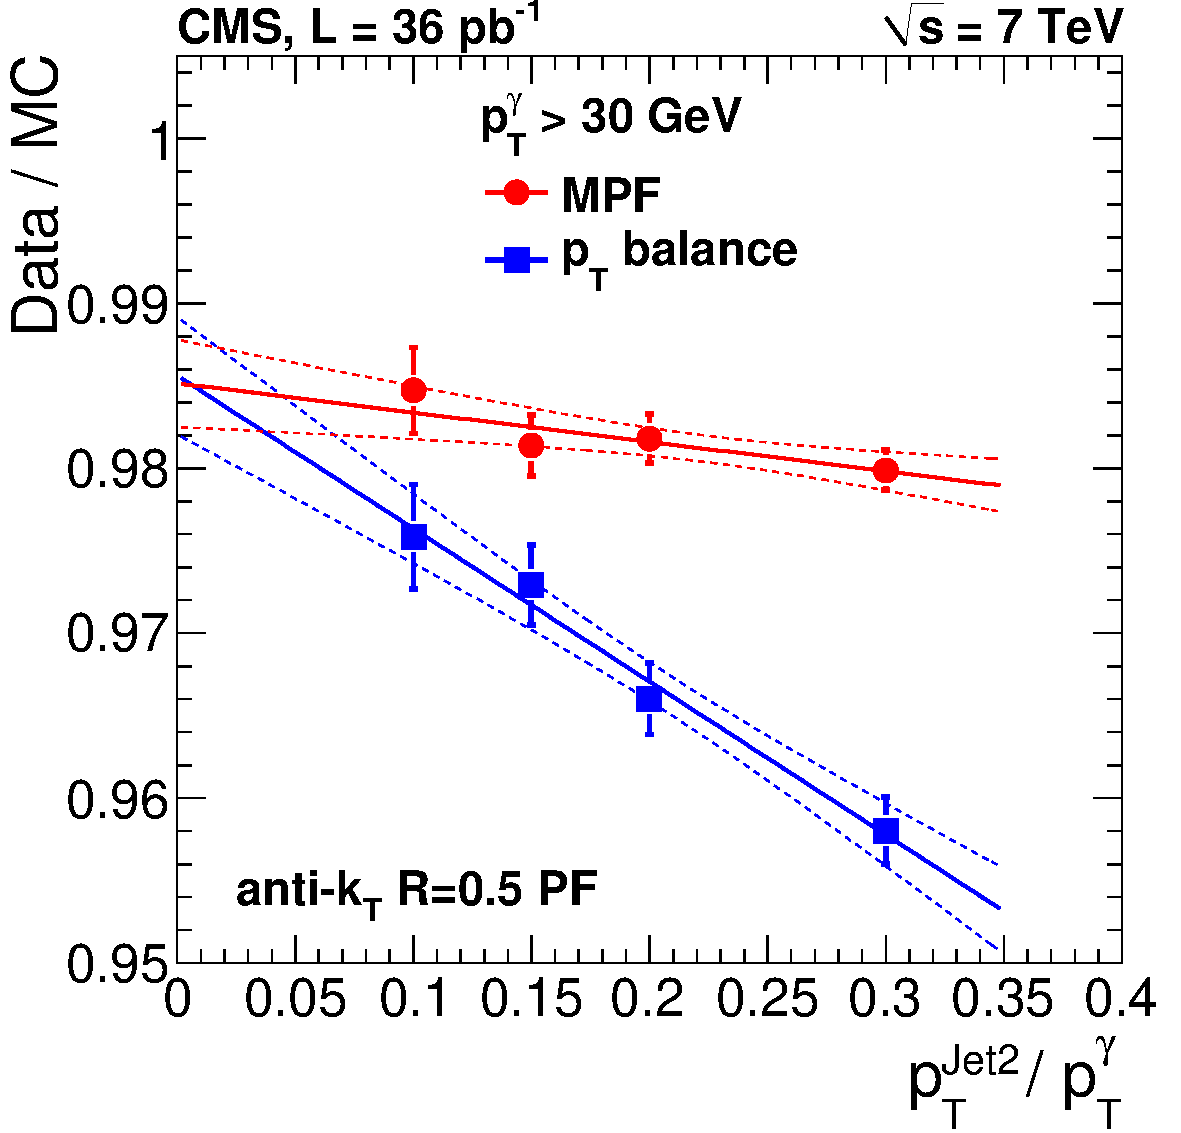
\includegraphics[width=0.45\textwidth]{Figures/JEC/MPF_pTbalance_vspT2nd_AK5}
    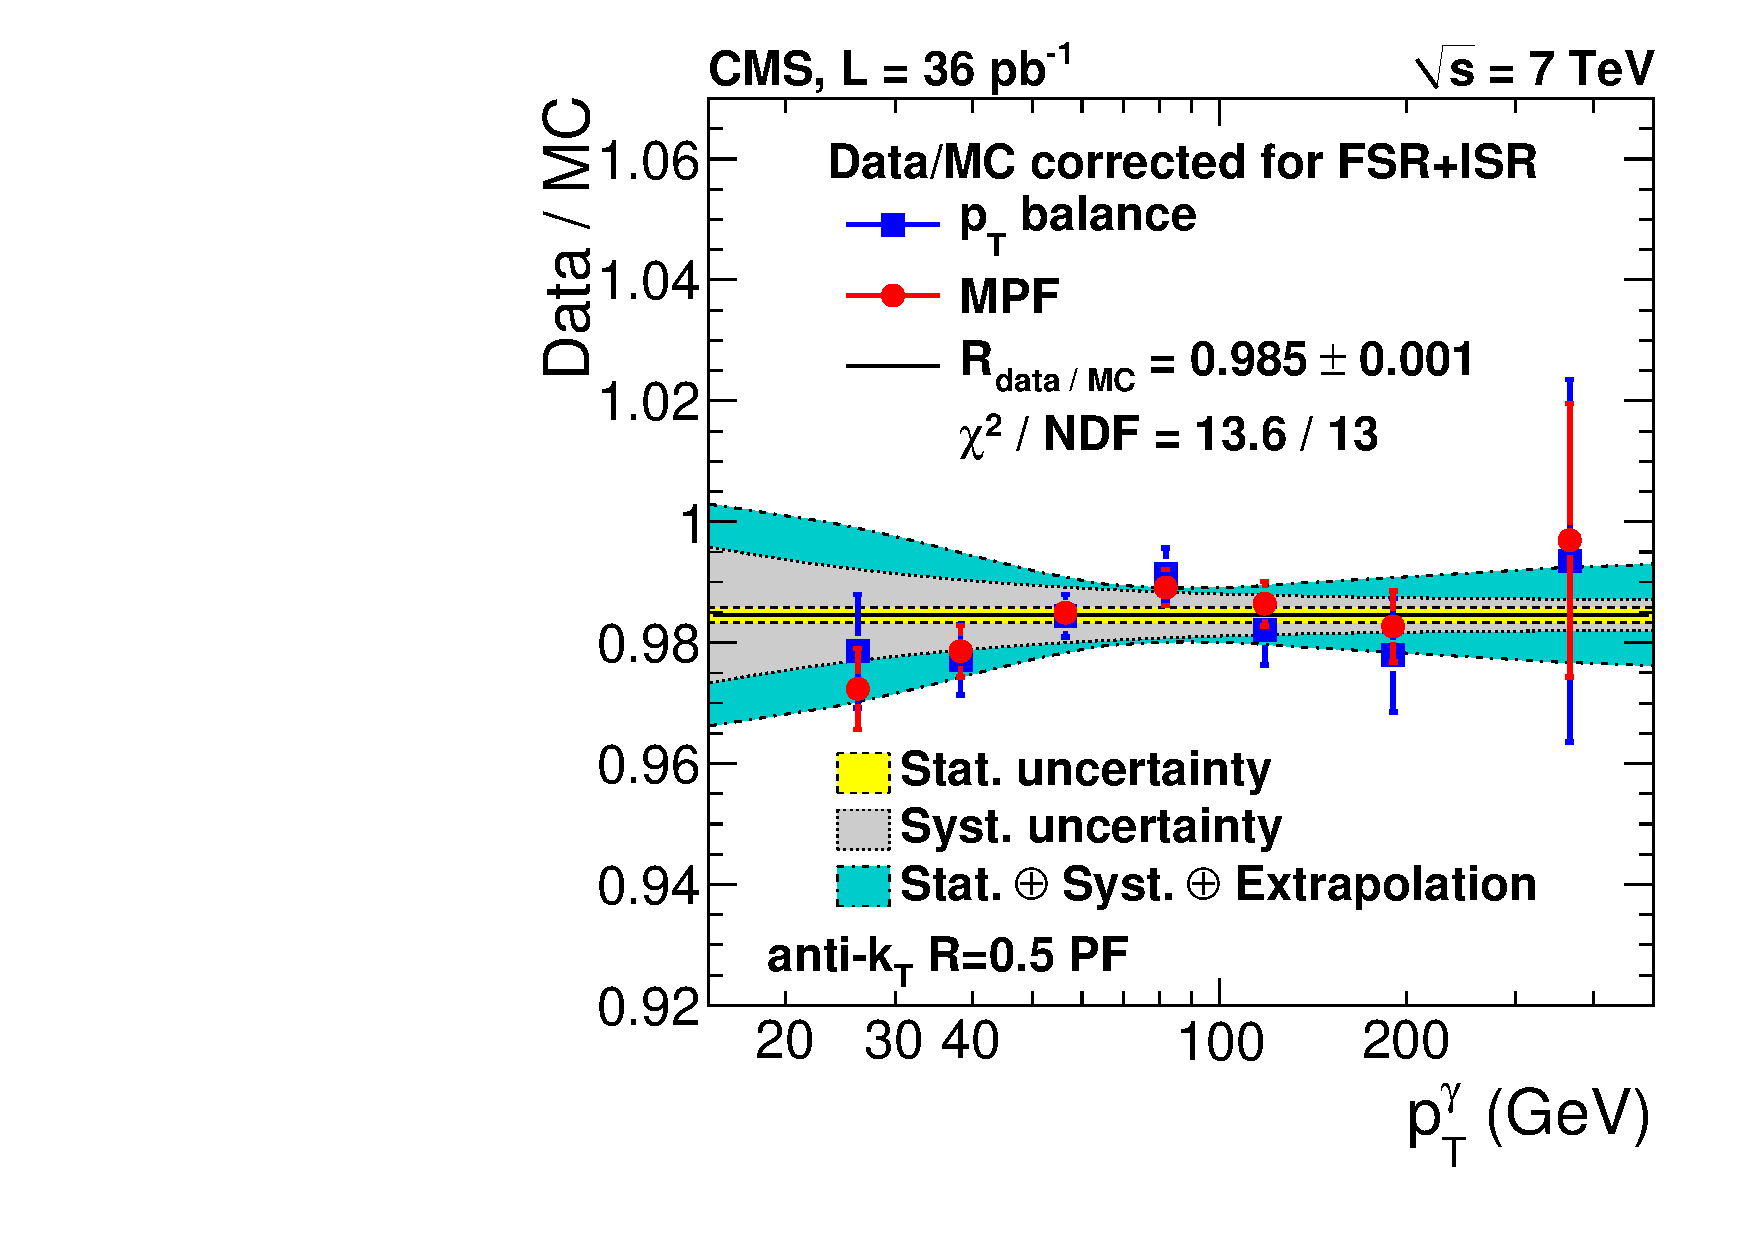
\includegraphics[width=0.45\textwidth]{Figures/JEC/FinalDataOverMC3_AK5}
    \caption{Left: dependence of the data/MC ratio of the jet energy response on the second jet \pt threshold. Right: data/MC ratio of the jet energy response, after extrapolation to zero second jet \pt, as a function of $\pt^\gamma$. Solid squares and solid circles correspond to the \pt-balancing and the MPF methods, respectively.}
    \label{fig:photon}
  \end{center}
\end{figure}

Figure~\ref{fig:photon} (left) shows the data/MC jet-energy-response ratio, relative to the $\gamma$ ECAL scale, extrapolated as a function of the threshold on the second jet \pt. In the \pt-balancing method, the secondary jet effect is more pronounced because it affects directly the transverse momentum balance between the photon and the leading jet. In the MPF method, the presence of the secondary jet(s) affects the measurement to a lesser extent, and mainly through the response difference between the leading jet and the secondary softer jet(s). For loose veto values, the ratio data/MC in both methods is lower than unity, while the agreement improves by tightening the veto. Figure~\ref{fig:photon} (right) shows the data/MC response ratio after the extrapolation to $\alpha=0$ for both MPF and \pt-balancing methods, as a function of $\pt^{\gamma}$. The two measurements are statistically uncorrelated to a good approximation and the two sets of points are fitted together with a constant value. The fit gives data/MC = $0.985 \pm 0.001$, relative to the $\gamma$ ECAL scale, which leads to an absolute response residual correction $C_\text{abs}=1/0.985=1.015$ (Eq.~(\ref{eq:jec_components})), constant in \pt.  

In addition to the $\gamma$+jets sample, the absolute jet energy response is also measured from the Z+jets sample. Figure~\ref{fig:ZJB} shows two characteristic response distributions in the $30\GeV<\pt^Z<60\GeV$ bin, as an example, measured from the $Z(\mu^+\mu^-)$+jets sample with the \pt-balancing and the MPF methods. The Z+jets samples cover the $\pt^Z$ range from 20\GeV to 200\GeV. 

\begin{figure}[ht!]
  \begin{center}
    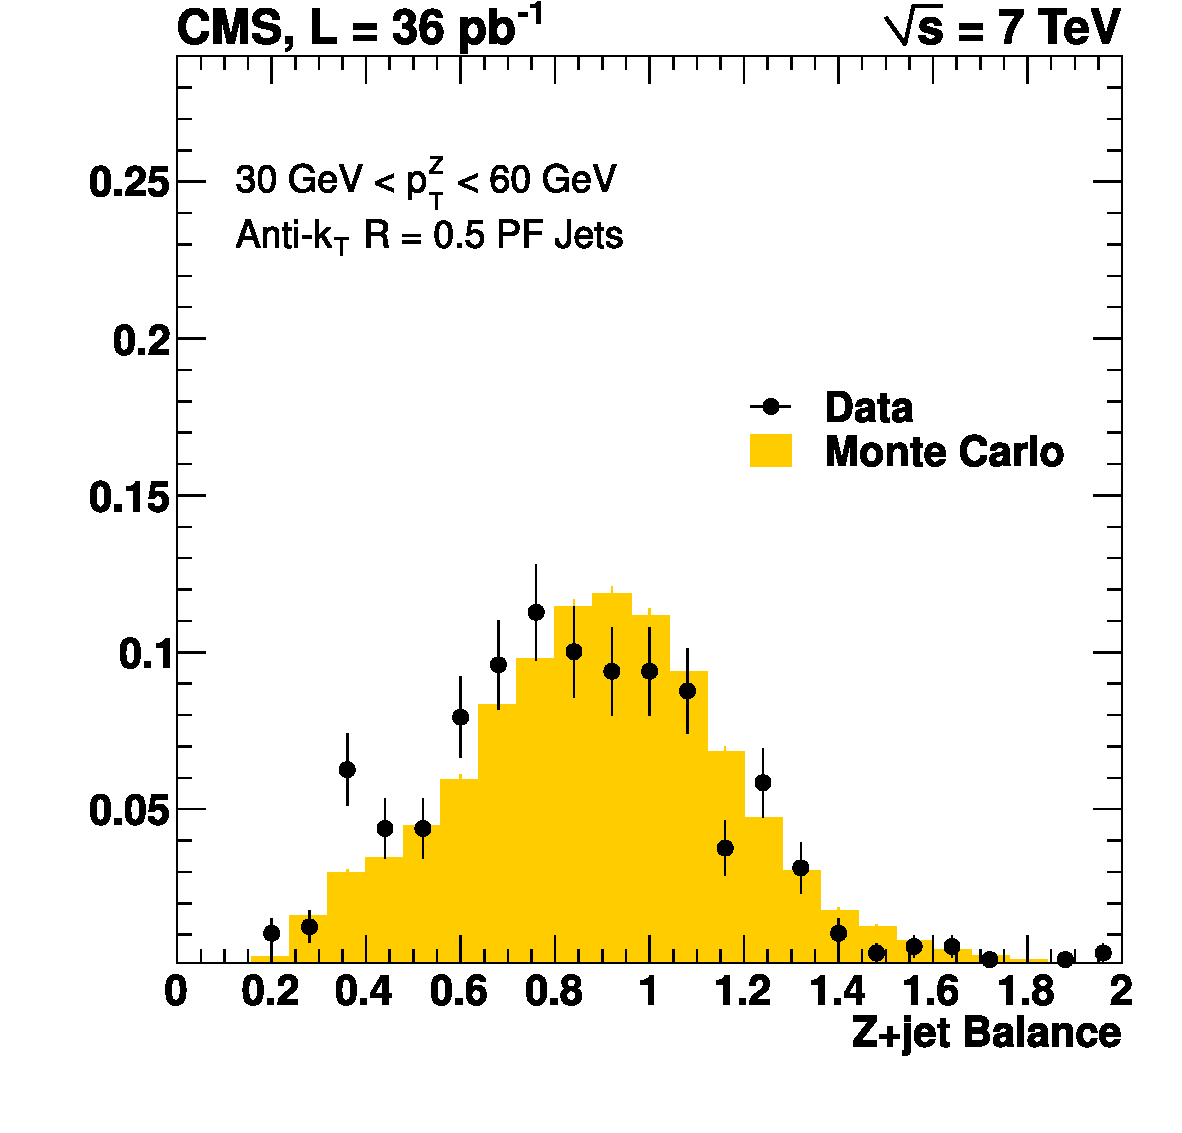
\includegraphics[width=0.45\textwidth]{Figures/JEC/jetresp_Pt30to60}
    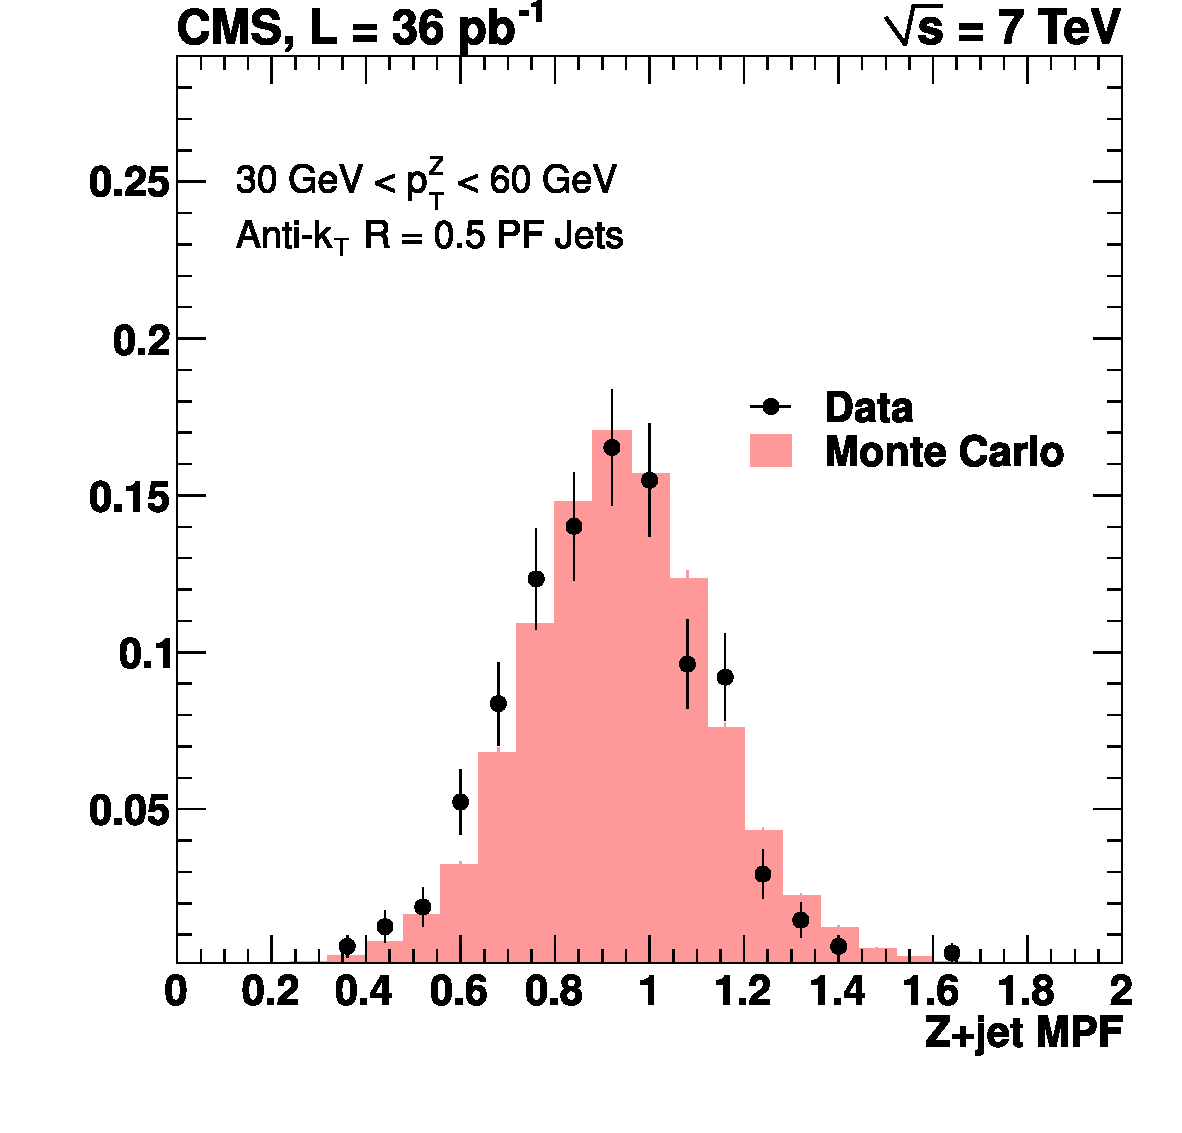
\includegraphics[width=0.45\textwidth]{Figures/JEC/mpfresp_Pt30to60}
    \caption{Left: jet energy response from $Z(\mu^+\mu^-)$+jets \pt-balancing in the bin $30<\pt^Z<60\GeV$. Right: jet energy response from $Z(\mu^+\mu^-)$+jets MPF in the bin $30<\pt^Z<60\GeV$.}
    \label{fig:ZJB}
  \end{center}
\end{figure}

\begin{figure}[ht!]
  \begin{center}
    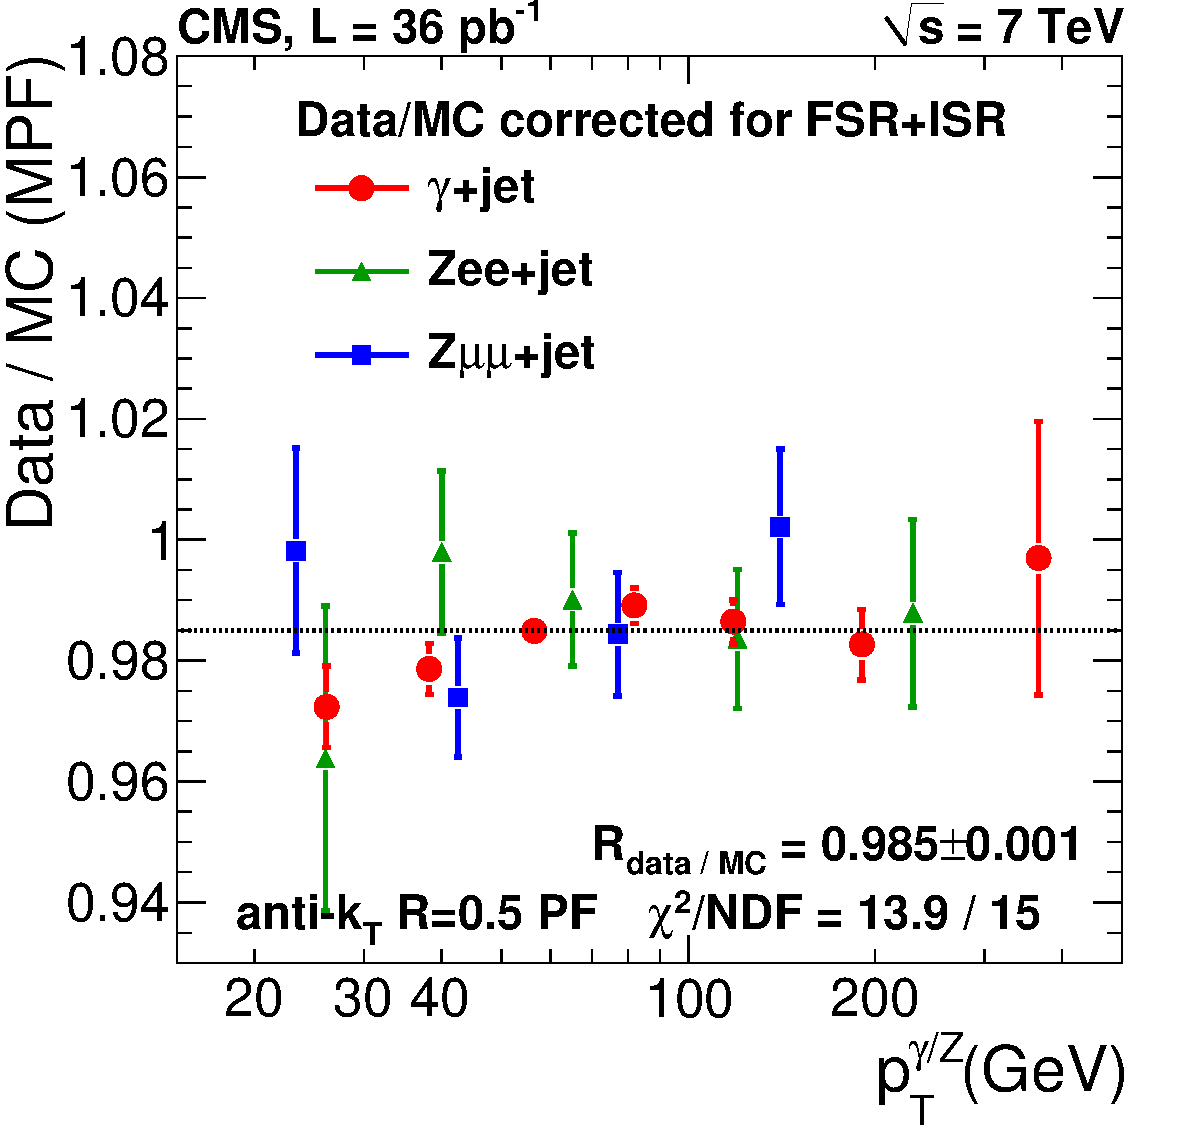
\includegraphics[width=0.45\textwidth]{Figures/JEC/FinalDataOverMC4_plusZ_AK5}
    \caption{Ratio of data over MC for the MPF response, as a function of $\pt^{\gamma,Z}$ in the photon+jet sample (circles), $Z(e^+e^-)$+jet sample (triangles) and $Z(\mu^+\mu^-)$+jet sample (squares).}
    \label{fig:dataMCAll}
  \end{center}
\end{figure}

In order to combine the results from the photon+jet and Z+jet samples, the more precise MPF method is employed identically in all relevant samples. Figure~\ref{fig:dataMCAll} shows the data/MC ratio as a function of $\pt^{\gamma,Z}$ after correcting for the final and initial state radiation differences between data and simulation (extrapolation to $\alpha=0$). Although the size of the Z+jets data sample is smaller than the $\gamma$+jets sample, the results from all samples are in good agreement, within the corresponding statistical uncertainties.

\subsubsection{Uncertainty Sources}

The uncertainty of the absolute jet energy scale measurement has six components: uncertainty in the MPF method for PF jets, photon energy scale, MC extrapolation beyond the reach of the available dataset, offset due to noise and pile-up at low-\pt (as discussed in Section~\ref{sec:offset_unc}), MC residuals (the level of closure of the MC correction in the MC), and the jet-by-jet matching residuals for CALO and JPT jets.  

{\bf MPF Uncertainty for PF Jets.} The MPF method is affected by several small uncertainties that mainly contribute at low \pt: flavour mapping, parton-to-particle level sensitivity, QCD background, secondary jets, and proton fragments. The various contributions are shown in Fig.~\ref{fig:jecuncert_mpf}.

\begin{figure}[ht!]
  \begin{center}
    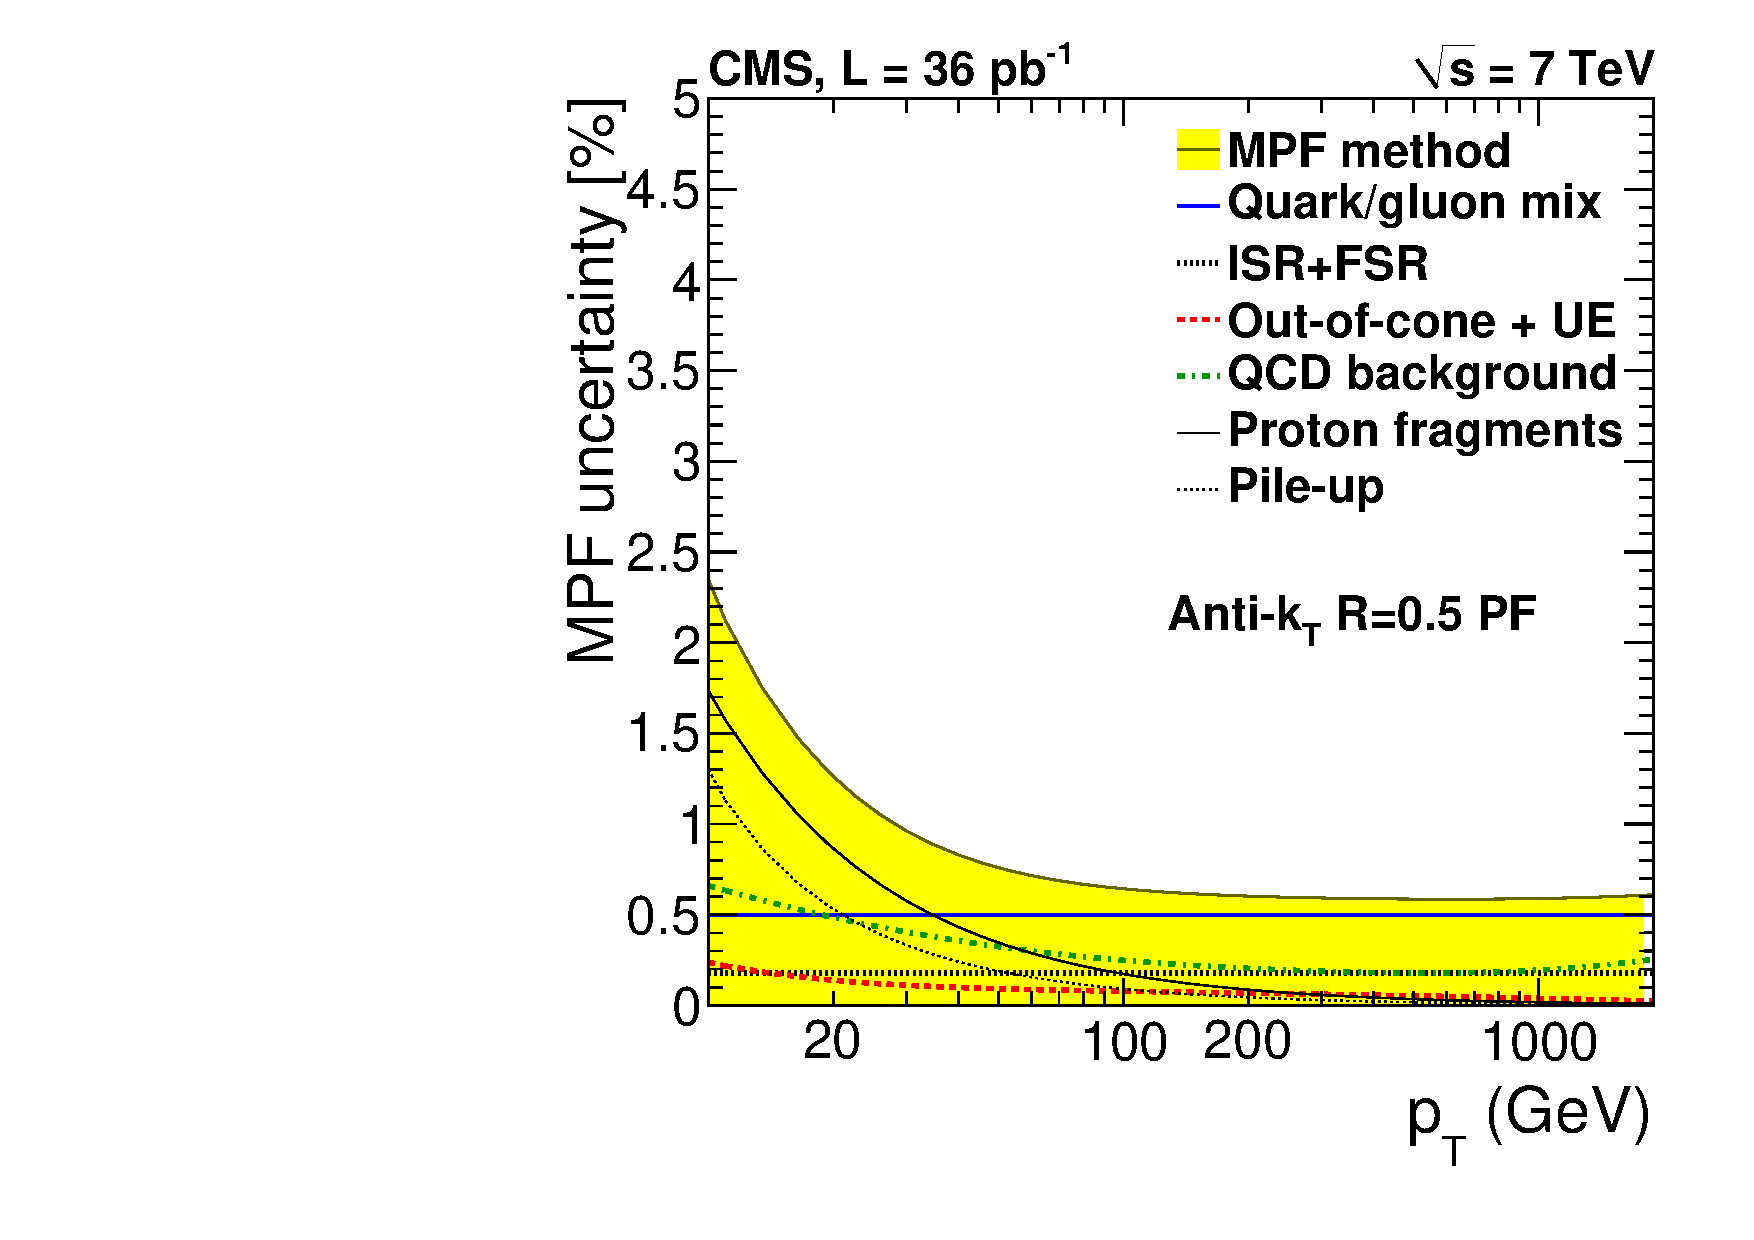
\includegraphics[width=0.45\textwidth]{Figures/JEC/JECUncert_MPF}
    \caption{Jet energy scale uncertainty in the MPF method for PF jets.}
    \label{fig:jecuncert_mpf}
  \end{center}
\end{figure}

The flavour mapping uncertainty accounts for the response difference between jets in the quark-rich $\gamma$+jets sample used to measure the absolute jet energy scale, and those in the reference, gluon-rich QCD multijet sample. This is estimated from the average quark-gluon response difference between {\sc PYTHIA6} and {\sc Herwig++} (Fig.~\ref{fig:flavor_herwigpythia}) in the region $30-150\GeV$. The latter is chosen because it is the \pt region best constrained by the available data. For PF jets, the flavour mapping uncertainty amounts to $\sim 0.5\%$.

By definition, the MPF response refers to the parton level because the photon is perfectly balanced in the transverse plane, against the outgoing partons. However, the default jet energy response refers to the particle level, which includes the UE and the hadronization effects. The parton-to-particle level response interpretation therefore is sensitive to the UE and the out-of-cone showering (OOC). The corresponding uncertainty is estimated from the simulation by using jets reconstructed with larger size parameter ($R=0.7$, more sensitive to UE and OOC) and comparing the extrapolation to the zero secondary jet activity with respect to the nominal size parameter ($R=0.5$). The resulting uncertainty has a weak \pt-dependence and is smaller than $0.2\%$. 

The dominant background for $\gamma$+jets events is the QCD dijet production where one leading jet fragments into a hard isolated $\pi^0\to\gamma+\gamma$. Such events can alter the measured \pt-balance because the leading neutral $\pi^0$ carries only a fraction of the initial parton energy. The QCD background uncertainty is estimated by repeating the measurement, using a loose and a tight photon identification, and is found to be negligible compared to the current statistical precision.

The MPF response at low \pt is sensitive to the undetected energy that leaks outside the forward calorimeter acceptance at $|\eta|>5$ (proton fragments). This results in an underestimation of the MPF response, compared to the true response. The uncertainty due to the undetected energy is taken from the simulation and is estimated to be $50\%$ of the difference between the MPF response and the true response. 

The secondary jet activity is found to be significantly different between data and MC, and it is corrected by extrapolating the data/MC ratio for the MPF and \pt-balance methods to zero secondary jet activity. The related uncertainty is estimated as half of the radiation bias correction applied to the MPF method.

{\bf Photon Energy Scale Uncertainty.} The MPF and \pt-balancing methods are directly sensitive to the uncertainty in the energy of the $\gamma$ used as a reference object. The $\gamma$ energy scale uncertainty is estimated to be $\sim 1\%$ based on studies presented elsewhere~\cite{EGM-10-003}.

{\bf Monte Carlo Extrapolation.} The in situ measurement of the absolute jet energy scale is feasible only in the \pt range where $\gamma$+jets data are available. For the current dataset this range extends to around $300\GeV$. However, the jet \pt range probed in the entire dataset is generally more than three times higher than in the $\gamma$+jets sample. In QCD dijet events, jets as high as $\pt = 1\TeV$ are observed. Because of the absence of data for direct response measurement at high \pt, the calibration relies on the simulation. Based on the data vs. MC comparison in the region of available $\gamma$+jets data, conclusions can be drawn for the extrapolation of the jet energy correction at the highest jet \pt.

\begin{figure}[ht!]
  \begin{center}
    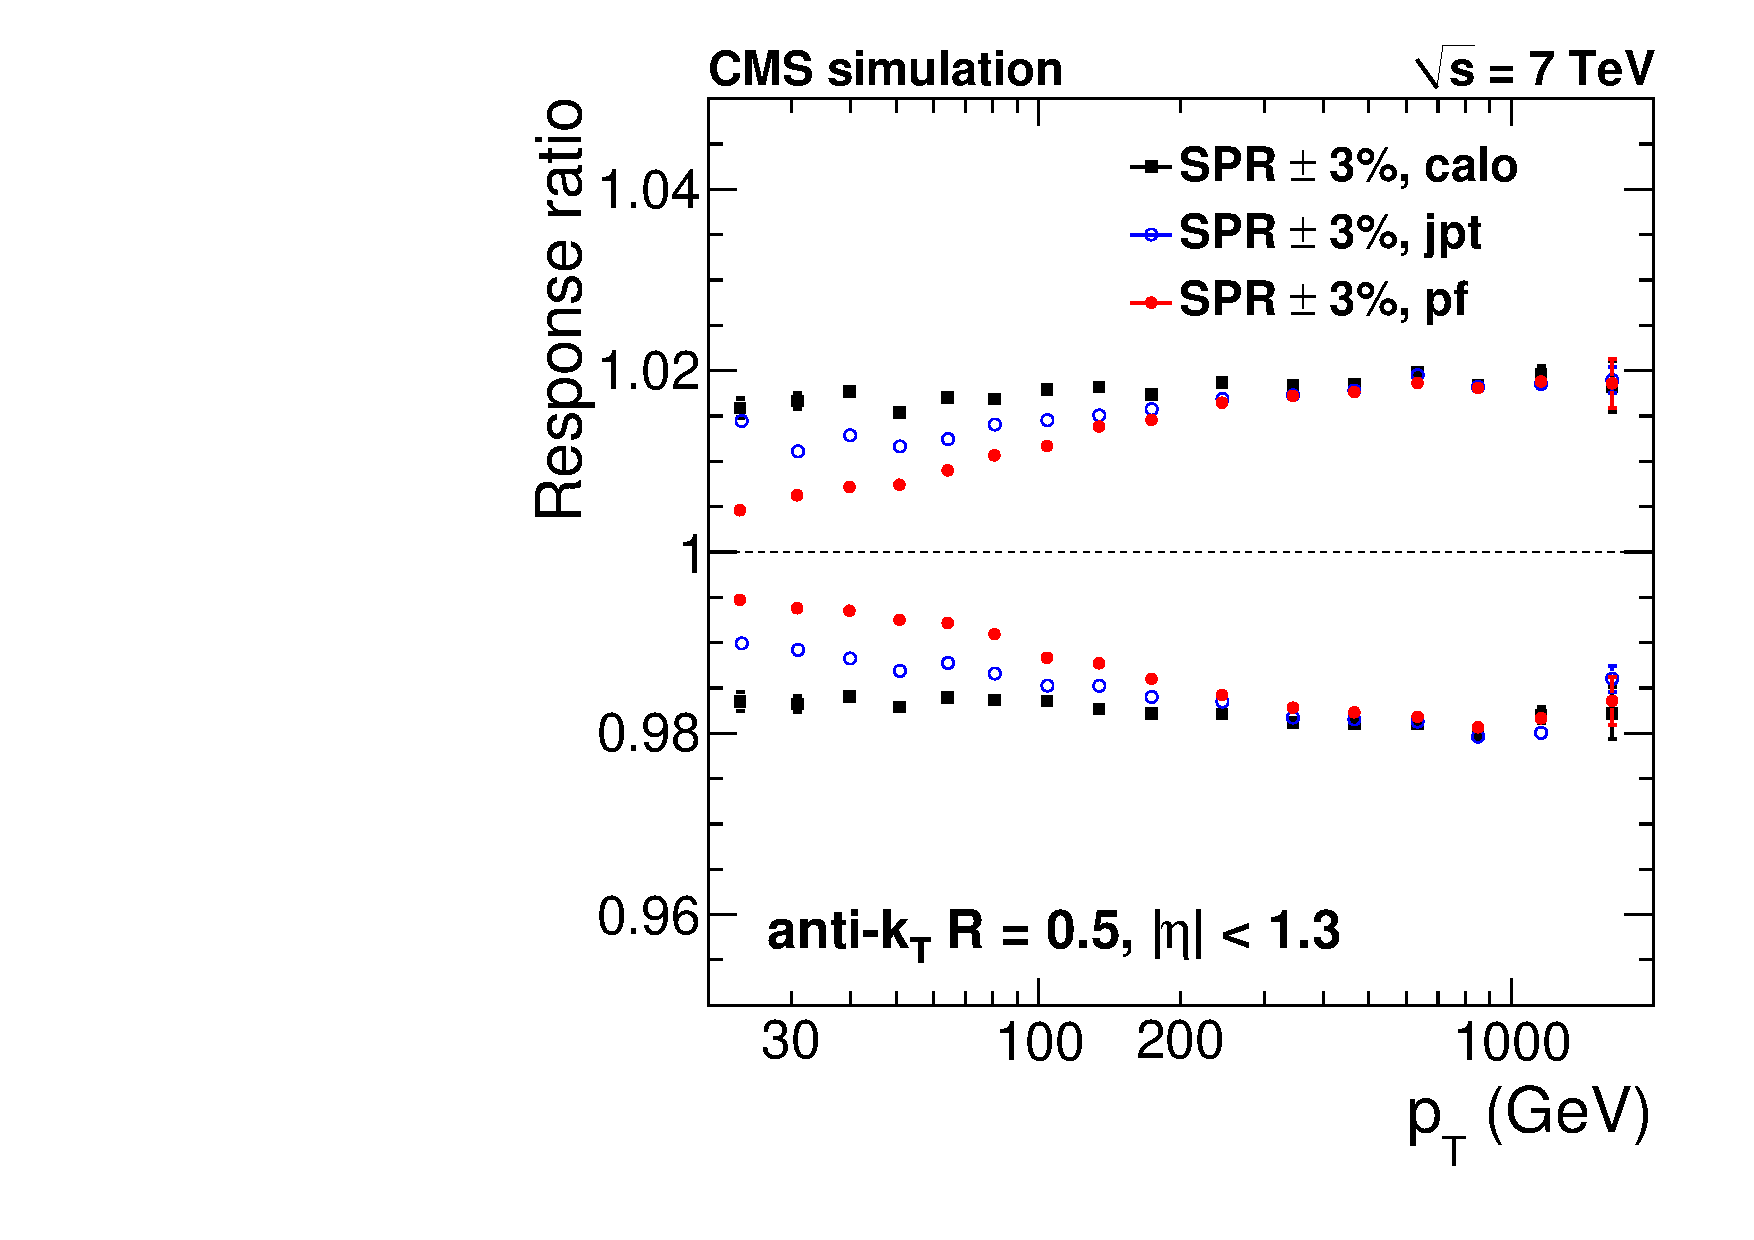
\includegraphics[width=0.45\textwidth]{Figures/JEC/singlepionresponse} 
    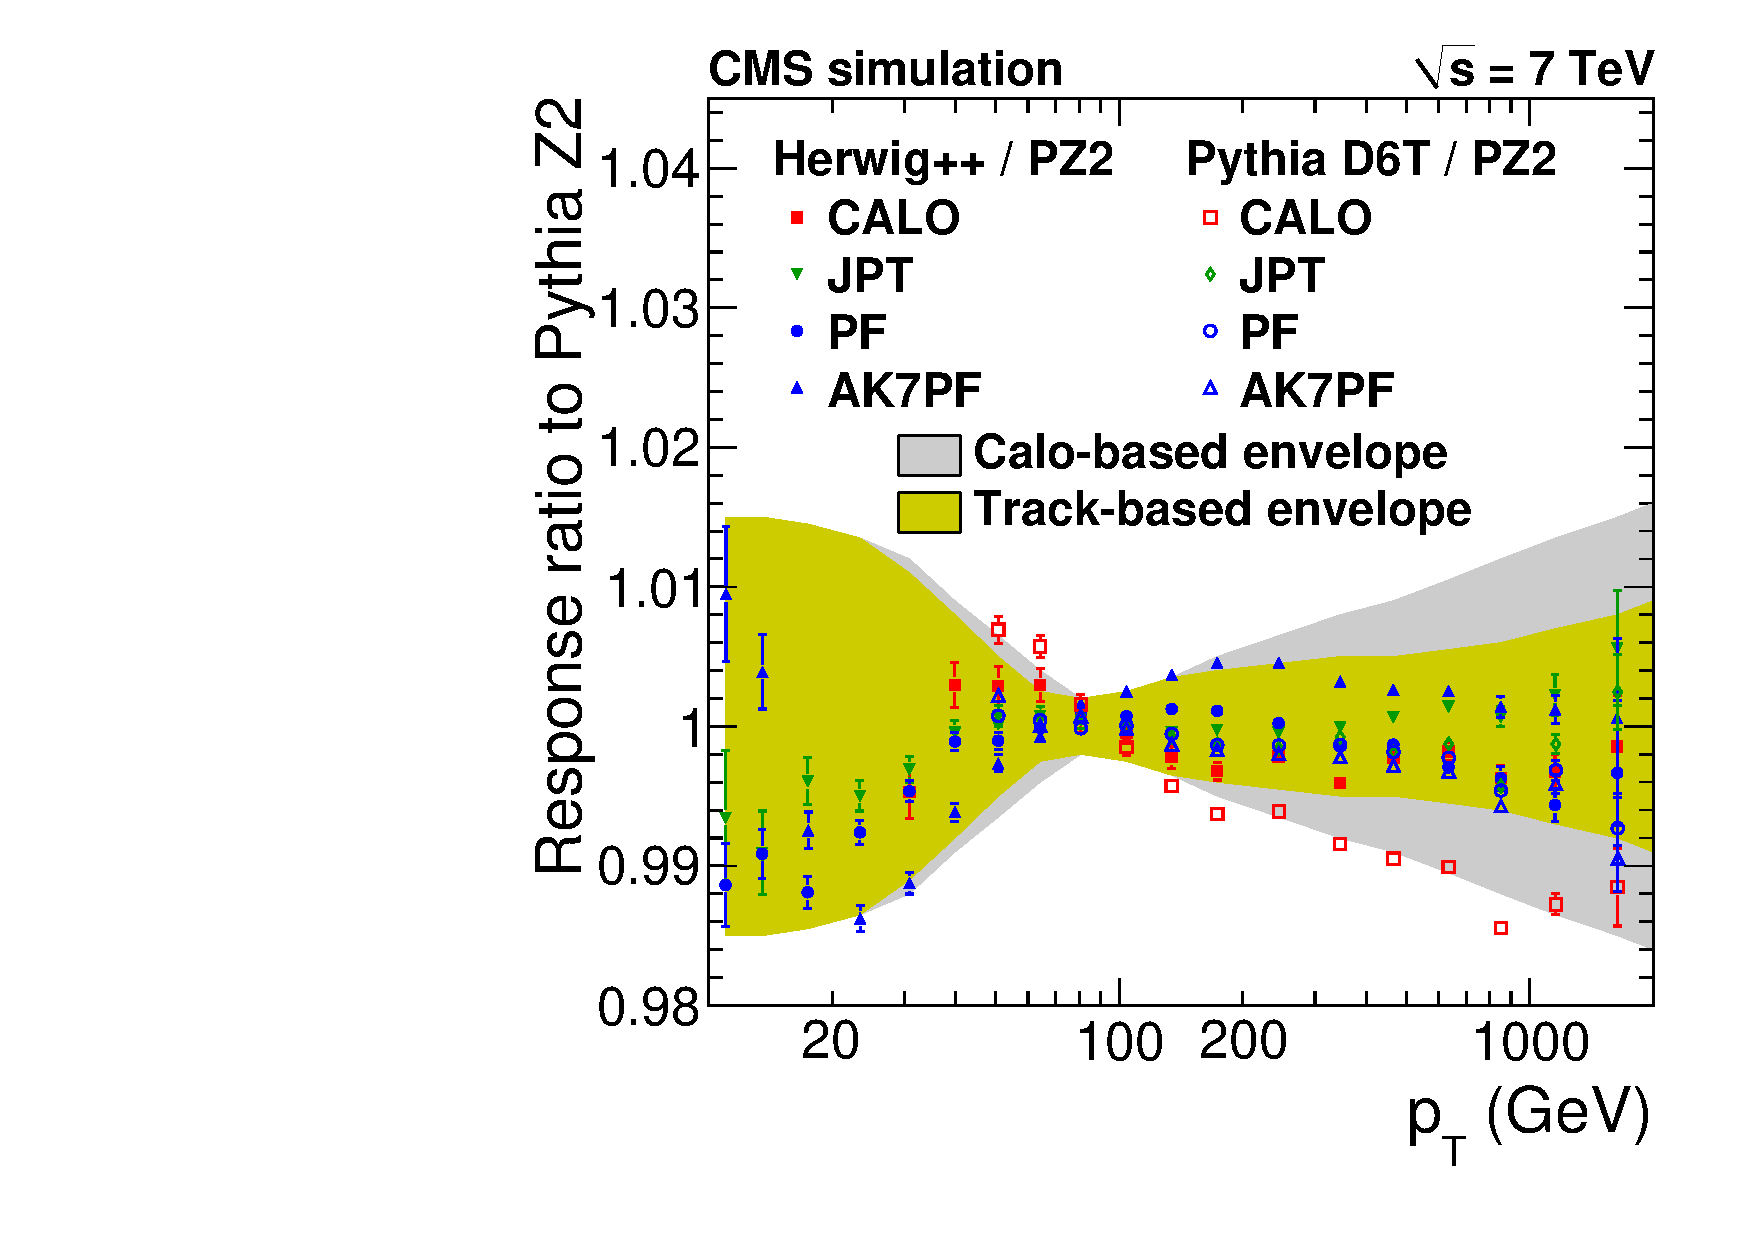
\includegraphics[width=0.45\textwidth]{Figures/JEC/highpt_envelope}
    \caption{Left: sensitivity of the jet energy response in $|\eta|<1.3$ to the single-particle response (SPR) uncertainty. Right: dependence of the jet energy response on the fragmentation model. Here AK7PF stands for PF jets reconstructed with the anti-$k_T$ algorithm with size parameter $R=0.7$.}
    \label{fig:FragSpr}
  \end{center}
\end{figure}

The simulation uncertainty for the high-\pt jets arises from two main sources: the single-particle response (SPR) for hadrons and the fragmentation modeling. The former is measured directly in data by using isolated tracks and comparing the energy deposited in the calorimeters with the momentum measured by the tracker. The currently available measurement~\cite{JME-10-008} indicates that the data/MC disagreement is less than 3\%. The SPR uncertainty is translated to a jet energy response uncertainty by modifying accordingly the simulation. Figure~\ref{fig:FragSpr} (left) shows the impact of the SPR uncertainty on the response of the different jet types, in the region $|\eta|<1.3$. For CALO jets, the induced uncertainty is roughly constant vs. \pt and approximately equal to 2\%. The track-based algorithms are less affected at low-\pt by the SPR uncertainty because the energy is primarily measured by the tracker. However, as the jet \pt increases and the track momentum measurement becomes less precise compared to the calorimetric measurement, the track-based jet types behave like CALO jets. The transition is smooth and is completed at jet $\pt\sim 300\GeV$. 

The other source of systematic uncertainty is related to the fragmentation properties, which include the parton shower and the hadronization simulation. Since jets are composite objects, realized as ``sprays" of highly collimated particles, and the calorimeter response is non-linear, the jet energy response depends on the number and the spectrum of the particles it consists of. The sensitivity to the fragmentation modelling is studied by generating QCD events from various MC generators which are then processed by the full simulation of the CMS detector. The MC generators employed are: {\sc PYTHIA6} (tunes D6T~\cite{D6T} and Z2) and {\sc Herwig++}\cite{HERWIG}. Figure~\ref{fig:FragSpr} (right) shows the response ratio of the various models with respect to {\sc PYTHIA6},with Z2 tune, which is the default. The differences between the models are negligible at $\pt\sim 80\GeV$, while they grow up to 1.5\% at low and high jet \pt. 

The combined MC uncertainty of the absolute jet energy response due to SPR and fragmentation is shown in Fig.~\ref{fig:highptUnc}.

\begin{figure}[ht!]
  \begin{center}
    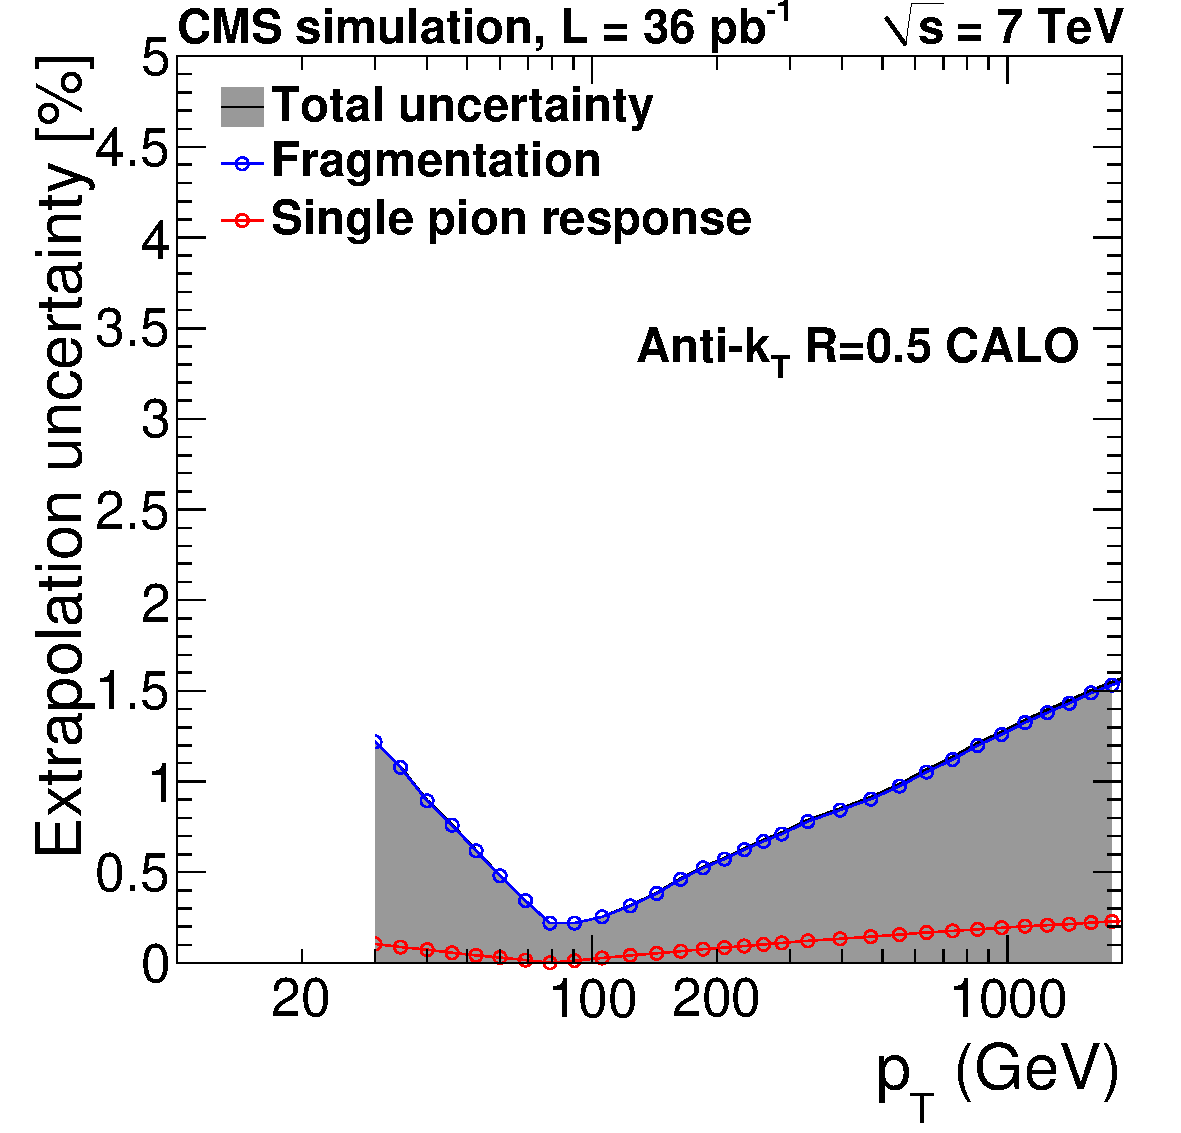
\includegraphics[width=0.45\textwidth]{Figures/JEC/JECUncert_HighPt_CALOAK5}
    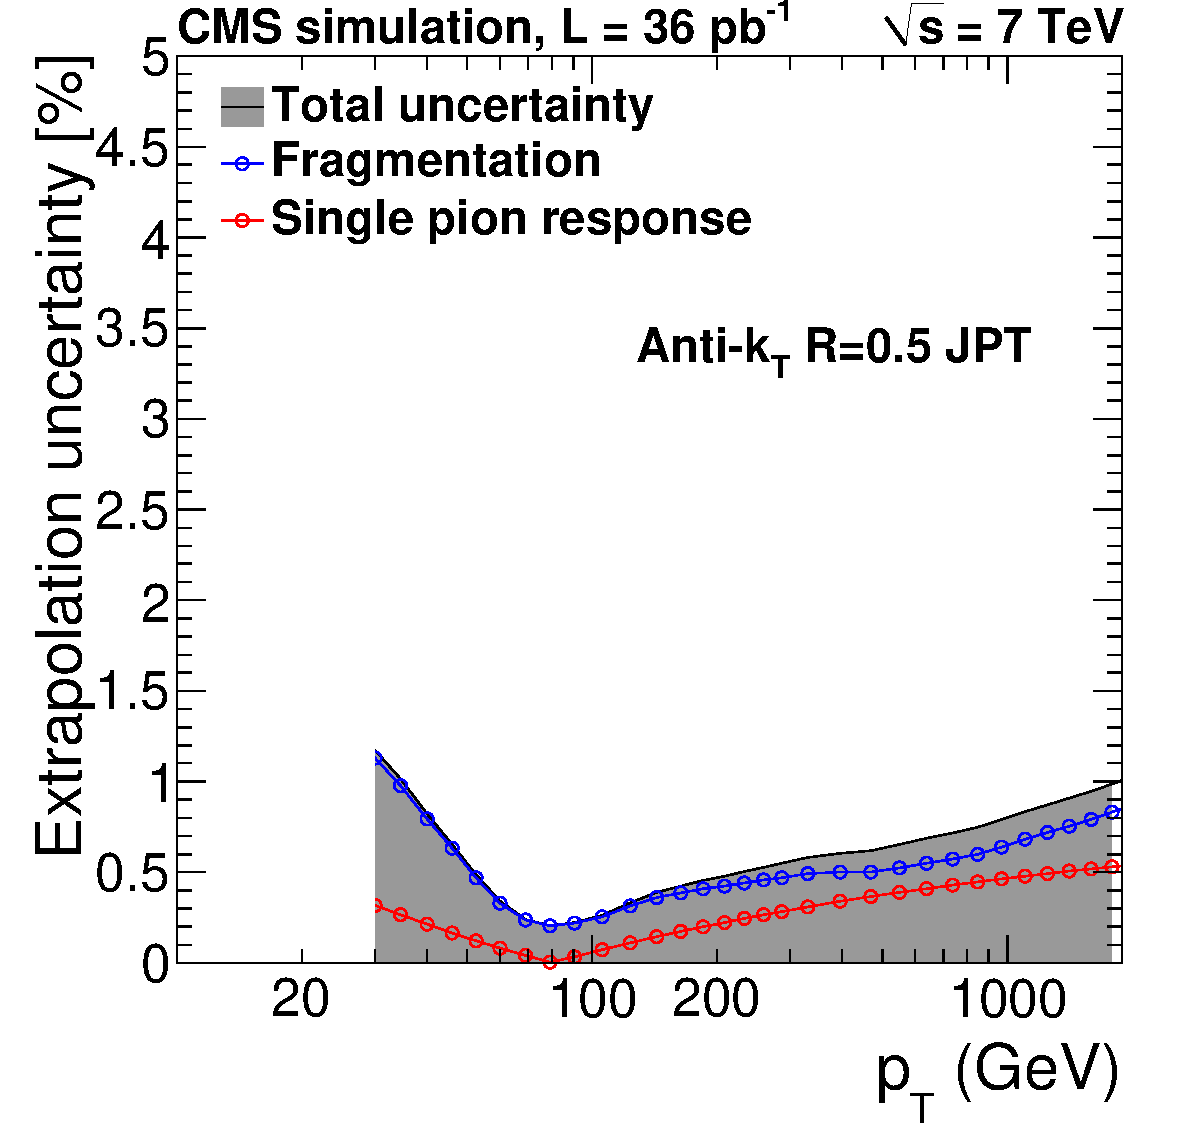
\includegraphics[width=0.45\textwidth]{Figures/JEC/JECUncert_HighPt_JPTAK5}
    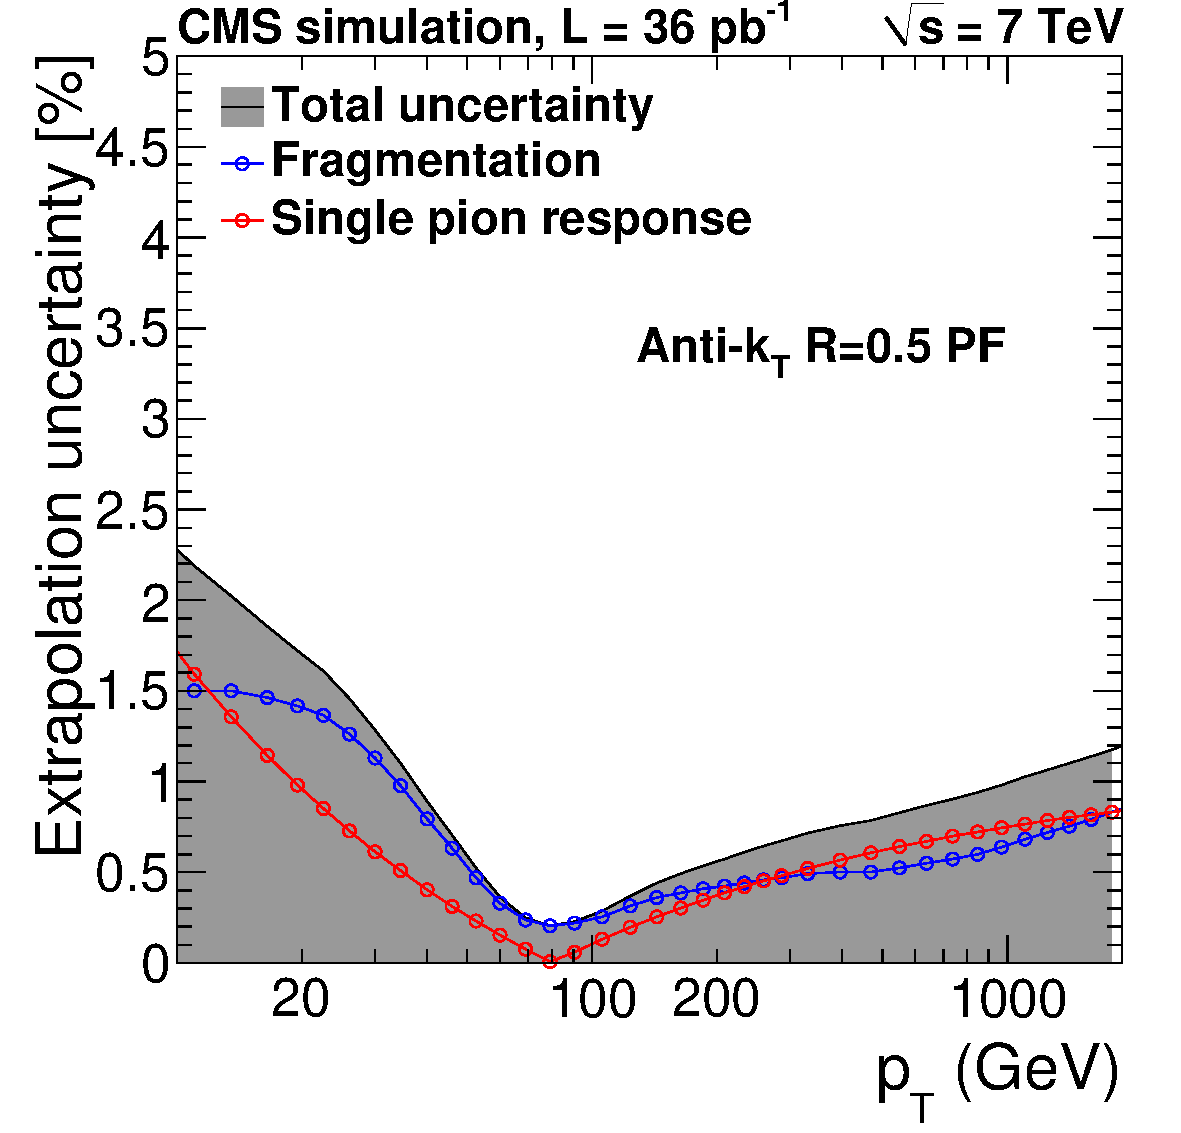
\includegraphics[width=0.45\textwidth]{Figures/JEC/JECUncert_HighPt_PFAK5}
    \caption{Uncertainty of the absolute jet energy response in the region $|\eta|<1.3$ related to the MC extrapolation for CALO, JPT and PF jets respectively. }
    \label{fig:highptUnc}
  \end{center}
\end{figure}

The particle-flow algorithm reconstructs individual particles, prior to jet clustering. This allows the detailed study of the PF jet composition in terms of charged hadrons, photons and neutral hadrons. In particular, the jet energy response is closely related to the energy fraction carried by the three major composition species. The purpose of this study is to demonstrate that the MC simulation is able to describe accurately the PF jet composition observed in data and therefore can be trusted to predict the PF jet response in the kinematic regions where the in situ measurement is not possible.

\begin{figure}[ht!]
  \begin{center}
    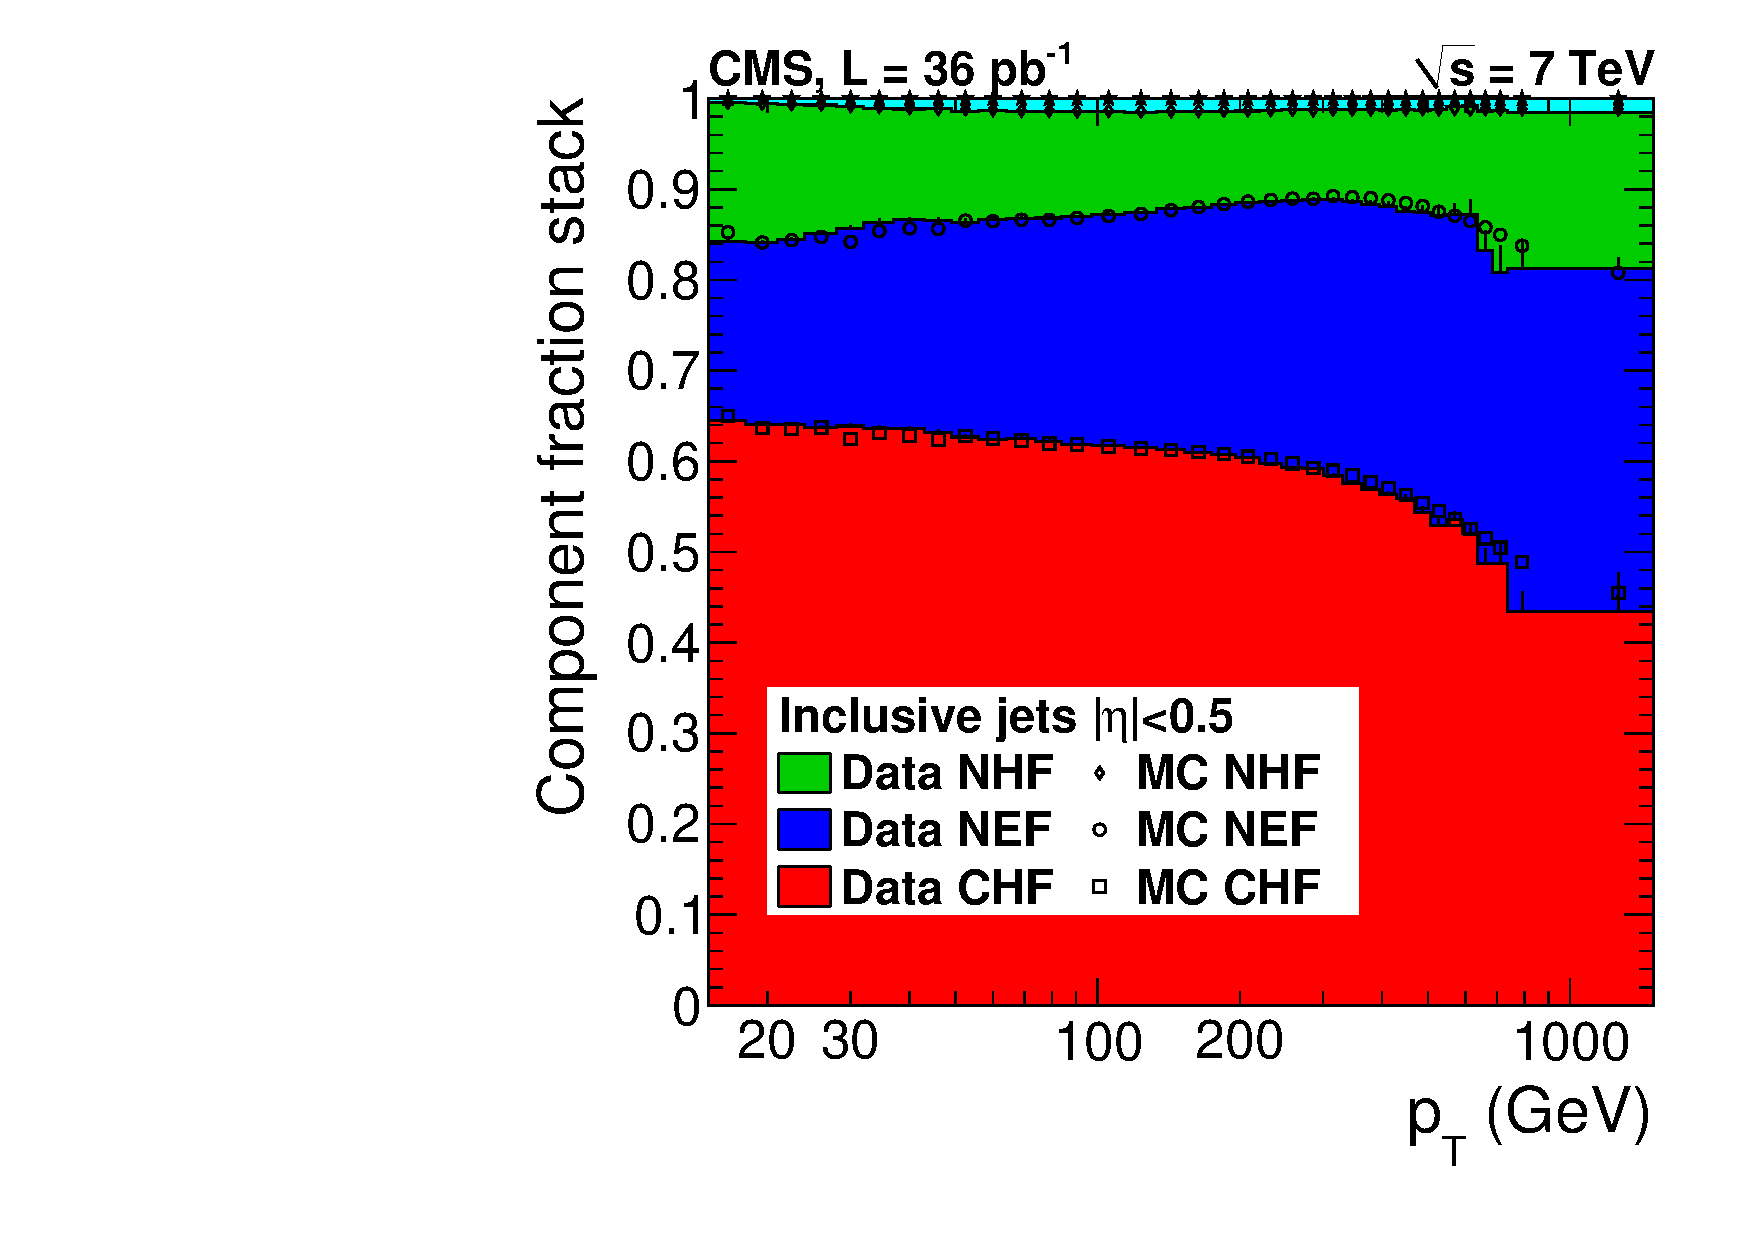
\includegraphics[width=0.45\textwidth]{Figures/JEC/jecChecks_fracstack_Rap0}
    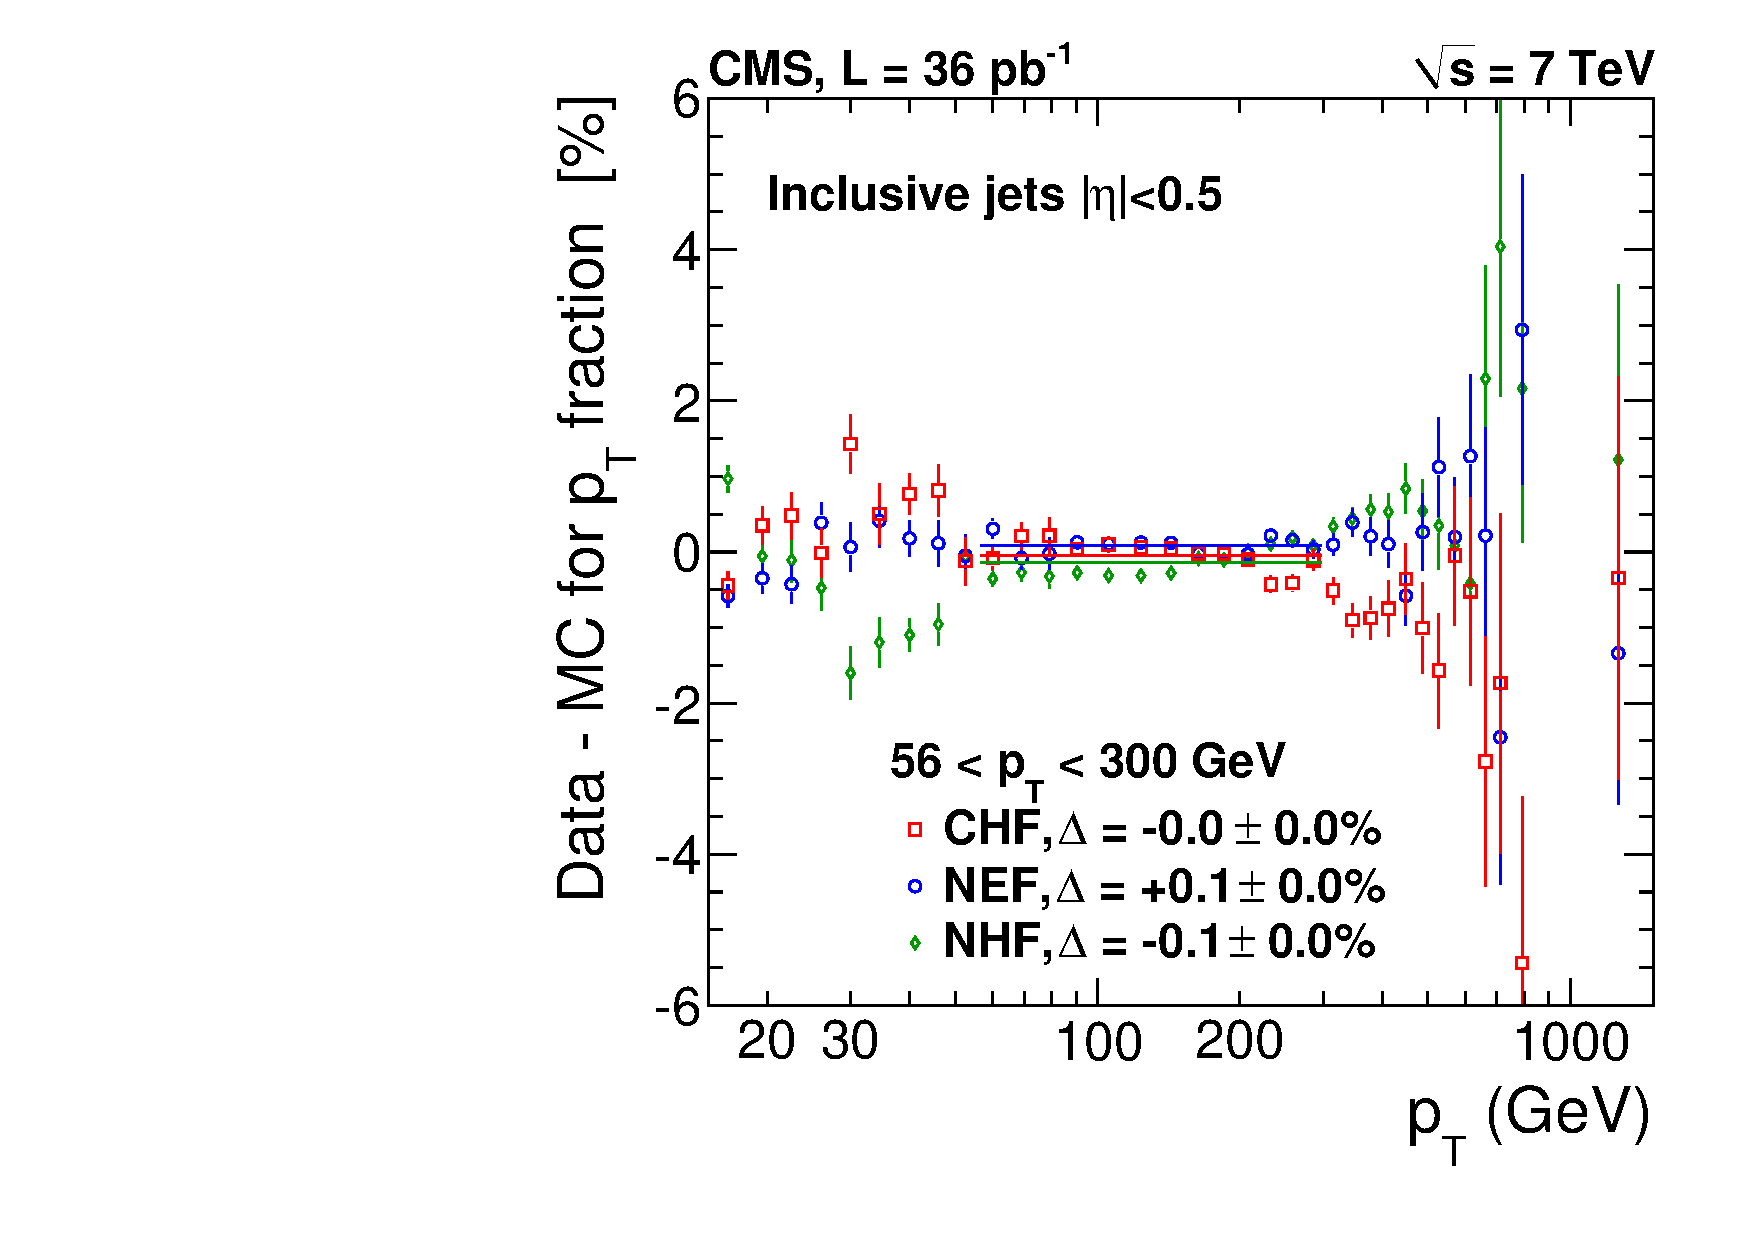
\includegraphics[width=0.45\textwidth]{Figures/JEC/jecChecks_fracDataMinusMC_Rap0.pdf}
    \caption{PF jet composition. Left: energy fraction carried by charged hadrons (CHF), photons (NEF), and neutral hadrons (NHF) as a function of jet \pt in the region $|\eta|<0.5$. The filled histograms and the markers represent the data and the simulation respectively. Right: \pt fraction difference between data and MC.}
    \label{fig:composition}
  \end{center}
\end{figure}

Figure~\ref{fig:composition} (left) shows the fraction of jet energy carried by the various particle types. Charged hadrons, photons, and neutral hadrons carry $\sim 65\%,\,20\%$, and $15\%$ of the jet energy respectively at low jet \pt, as expected from the general properties of the fragmentation process. As the jet \pt increases, charged hadrons become more energetic and more collimated, while the tracking efficiency and momentum resolution worsen. This increases the probability for a charged hadron to leave detectable energy only in the calorimeters and to be classified either as a neutral electromagnetic object (photon) or as a neutral hadron. Therefore, for higher jet \pt, the energy fraction carried by photons and neutral hadrons is increased. The excellent agreement between data and simulation quantified in Fig.~\ref{fig:composition} (right) proves that the simulation can be safely trusted to predict the absolute jet energy response. 

\begin{figure}[ht!]
  \begin{center}
    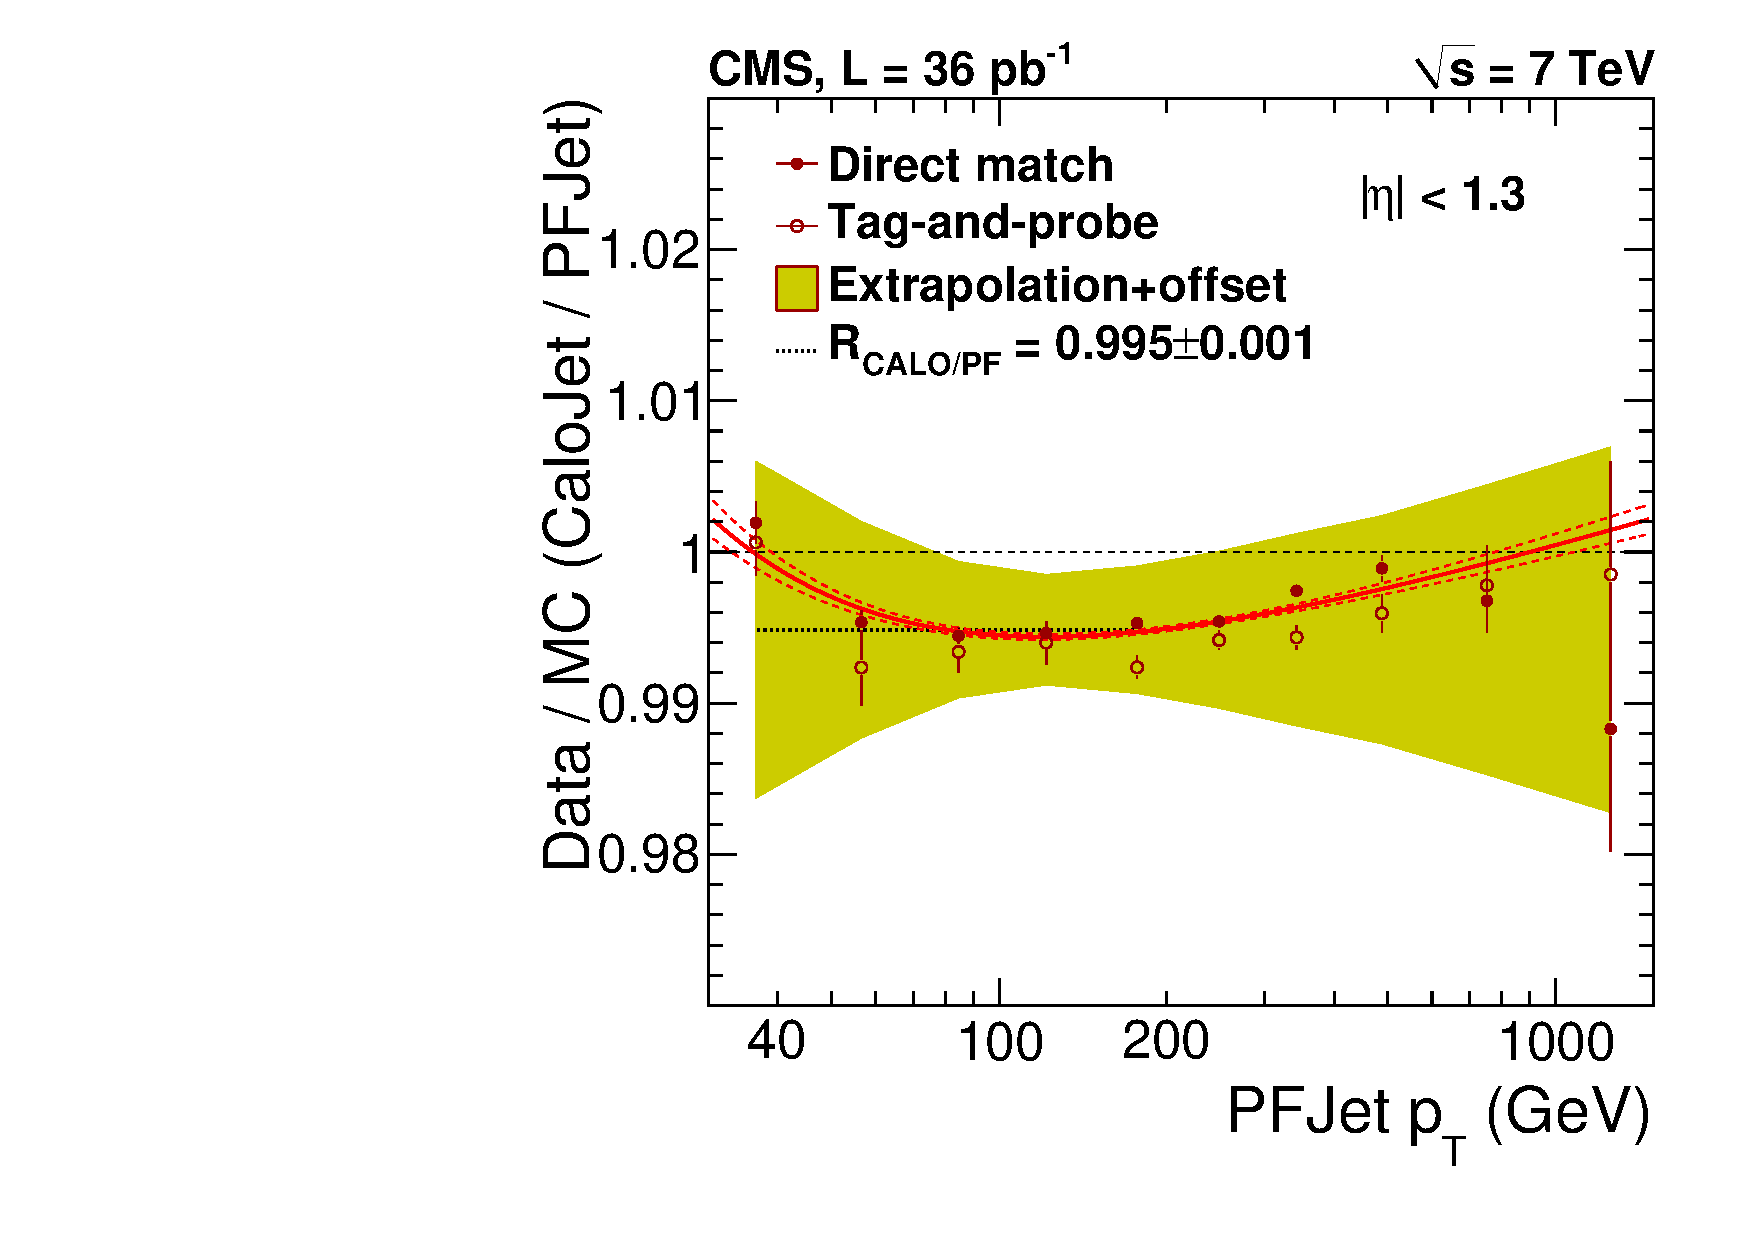
\includegraphics[width=0.45\textwidth]{Figures/JEC/jetmatch013_calopf.pdf}
    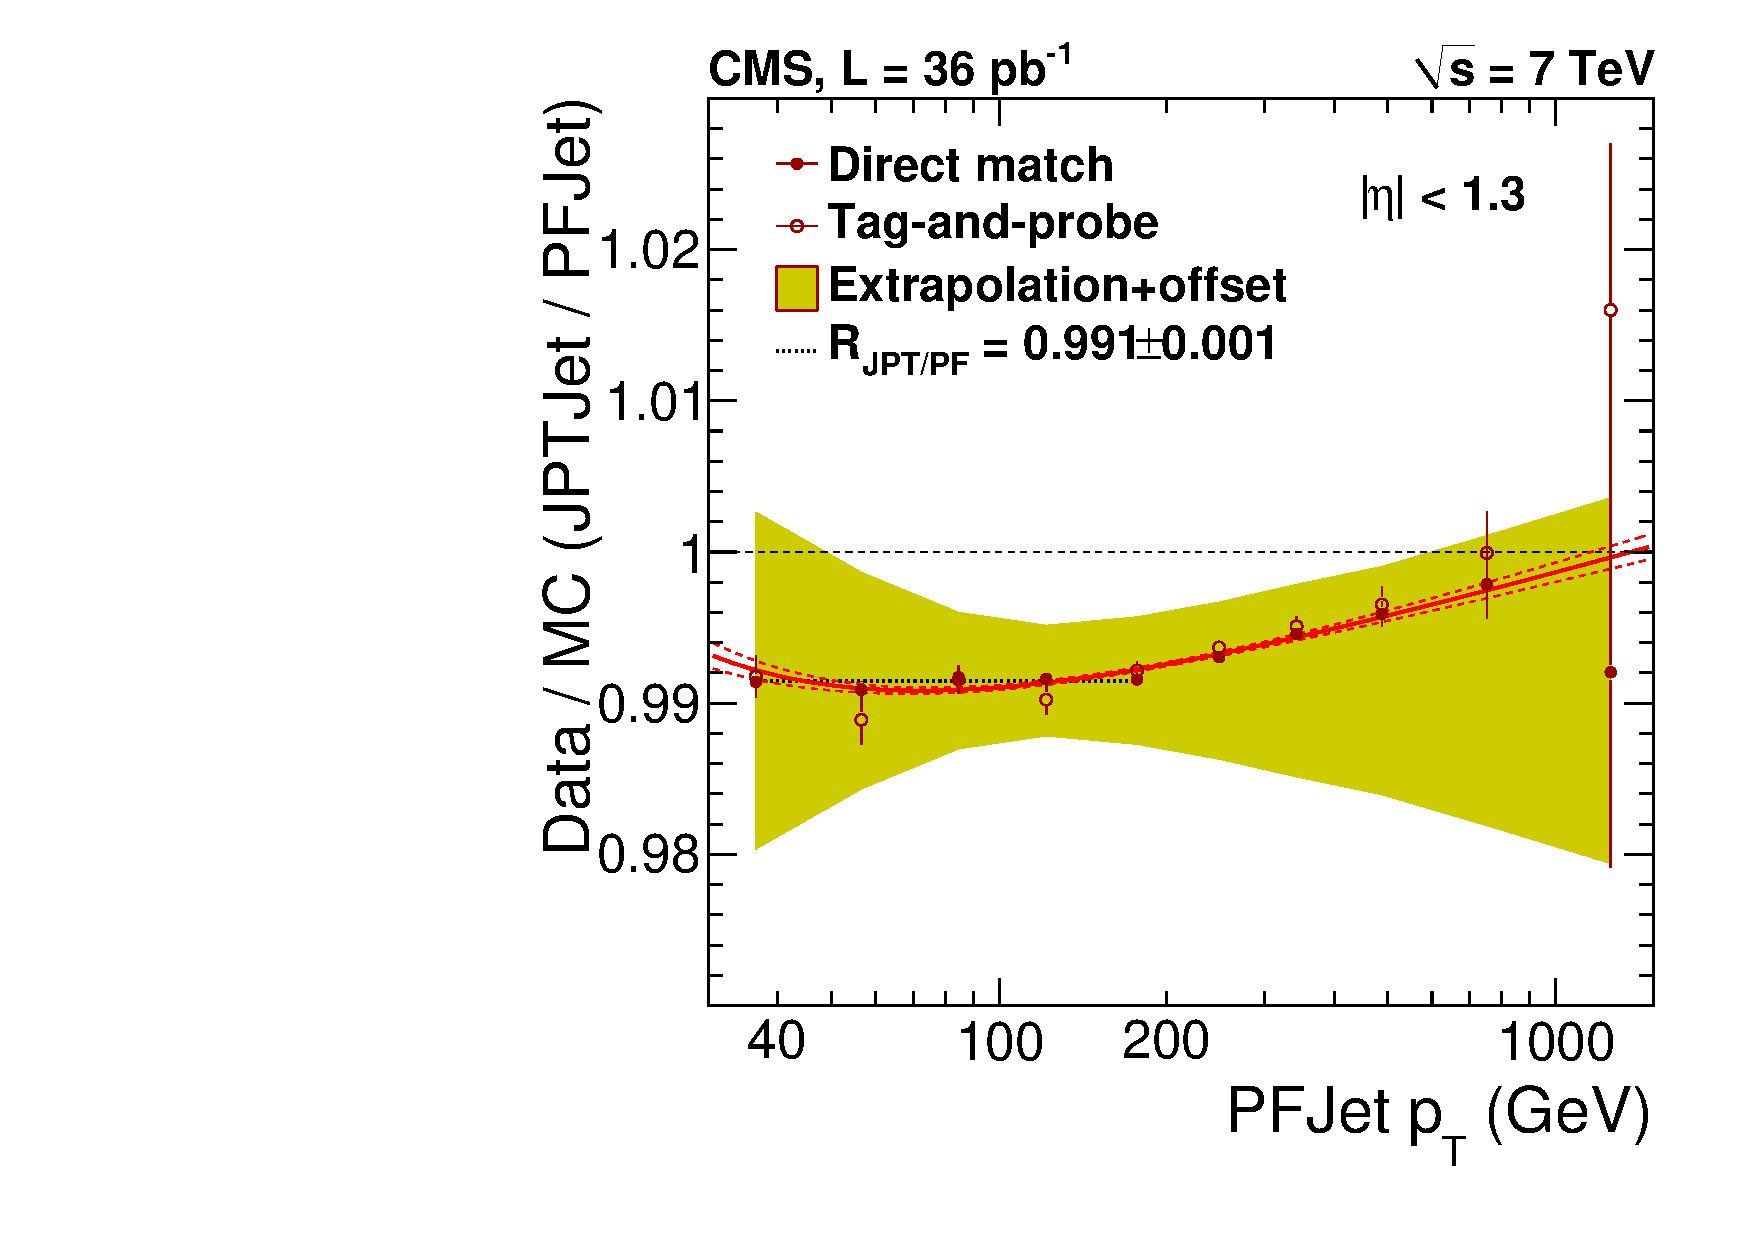
\includegraphics[width=0.45\textwidth]{Figures/JEC/jetmatch013_jptpf.pdf}
    \caption{Left: CALO vs. PF jet \pt response ratio between data and MC simulation. Right: JPT vs. PF jet \pt response ratio between data and MC simulation. The solid circles correspond to direct matching in the $\eta-\phi$ space and the open circles correspond to a tag (PF jet) and probe (CALO/JPT jet) method.}
    \label{fig:caloVsPF}
  \end{center}
\end{figure}

{\bf Jet-by-Jet Matching.} Once the jet energy scale is established for PF jets, the estimated uncertainties are transfered to the other jet types. This is done by direct jet-by-jet comparison between different jet types in the QCD dijet sample. The PF and CALO (JPT) jets are spatially matched in the $\eta,\,\phi$ space by requiring $\DeltaR<0.25$. For the matched jet pairs the relative response of CALO (JPT) jets $\pt^{CALO}/\pt^{PF}$ ($\pt^{JPT}/\pt^{PF}$) is measured as a function of $\pt^{PF}$ (the study is described in detail in Ref.~\cite{JME-10-003}). A cross-check of the direct jet matching is done with a tag-and-probe method in dijet events, with the PF jet being the tag object and the CALO/JPT jets being the probe objects. The results are summarized in Fig.~\ref{fig:caloVsPF} where the response ratio data/MC of the CALO and JPT response relative to the PF jets is shown. The observed disagreement is at the level of $0.5\%$, indicating that the precision of the CALO and JPT calibration is comparable to that of the PF jets. The observed $0.5\%$ level of data/MC disagreement is taken into account as an additional systematic uncertainty for CALO and JPT jets.

\subsubsection{Uncertainty}

As described in the previous sections, the absolute jet energy response is measured in situ for PF jets with the MPF method in $\gamma$/Z+jets events. The systematic uncertainties related to the measurement itself are summarized in Fig.~\ref{fig:jecuncert_mpf}. The estimation of the systematic uncertainty in the kinematic region beyond the reach of the $\gamma$+jets sample is based on the simulation and its sensitivity to the single-particle response and the fragmentation models. In addition, the uncertainty on the $\gamma$ energy scale needs to be taken into account since the jet energy response is measured relative to the $\gamma$ scale. The direct jet-by-jet spatial matching, allows the transfer of the PF jet-energy- scale uncertainty to the other jet types (CALO, JPT). Finally, a flavour uncertainty is assigned from the response differences between the quark and gluon originated jets. These are taken from Fig.~\ref{fig:flavor_herwigpythia} and cover the absolute scale uncertainty in physics samples with a different flavour mixture than the reference QCD multijet sample. 

Figure~\ref{fig:absunc} shows the absolute energy scale uncertainties for the three jet types, combined with the offset correction uncertainty corresponding to the average number of pile-up events in the datasets considered for this paper. The low jet \pt threshold indicates the minimum recommended \pt for each jet type: 30\GeV, 20\GeV, and 10\GeV for CALO, JPT, and PF jets respectively. At low jet \pt the offset uncertainty dominates with significant contribution from the MC truth and jet-by-jet matching residuals. At the intermediate jet \pt, where enough data for the in situ measurements are available, the $\gamma$ energy scale uncertainty dominates. At high jet \pt, the uncertainty due to the MC extrapolation is dominant. Overall, the absolute jet energy scale uncertainty for all jet types is smaller than 2\% for $\pt>40\GeV$. 

\begin{figure}[ht!]
  \begin{center}
    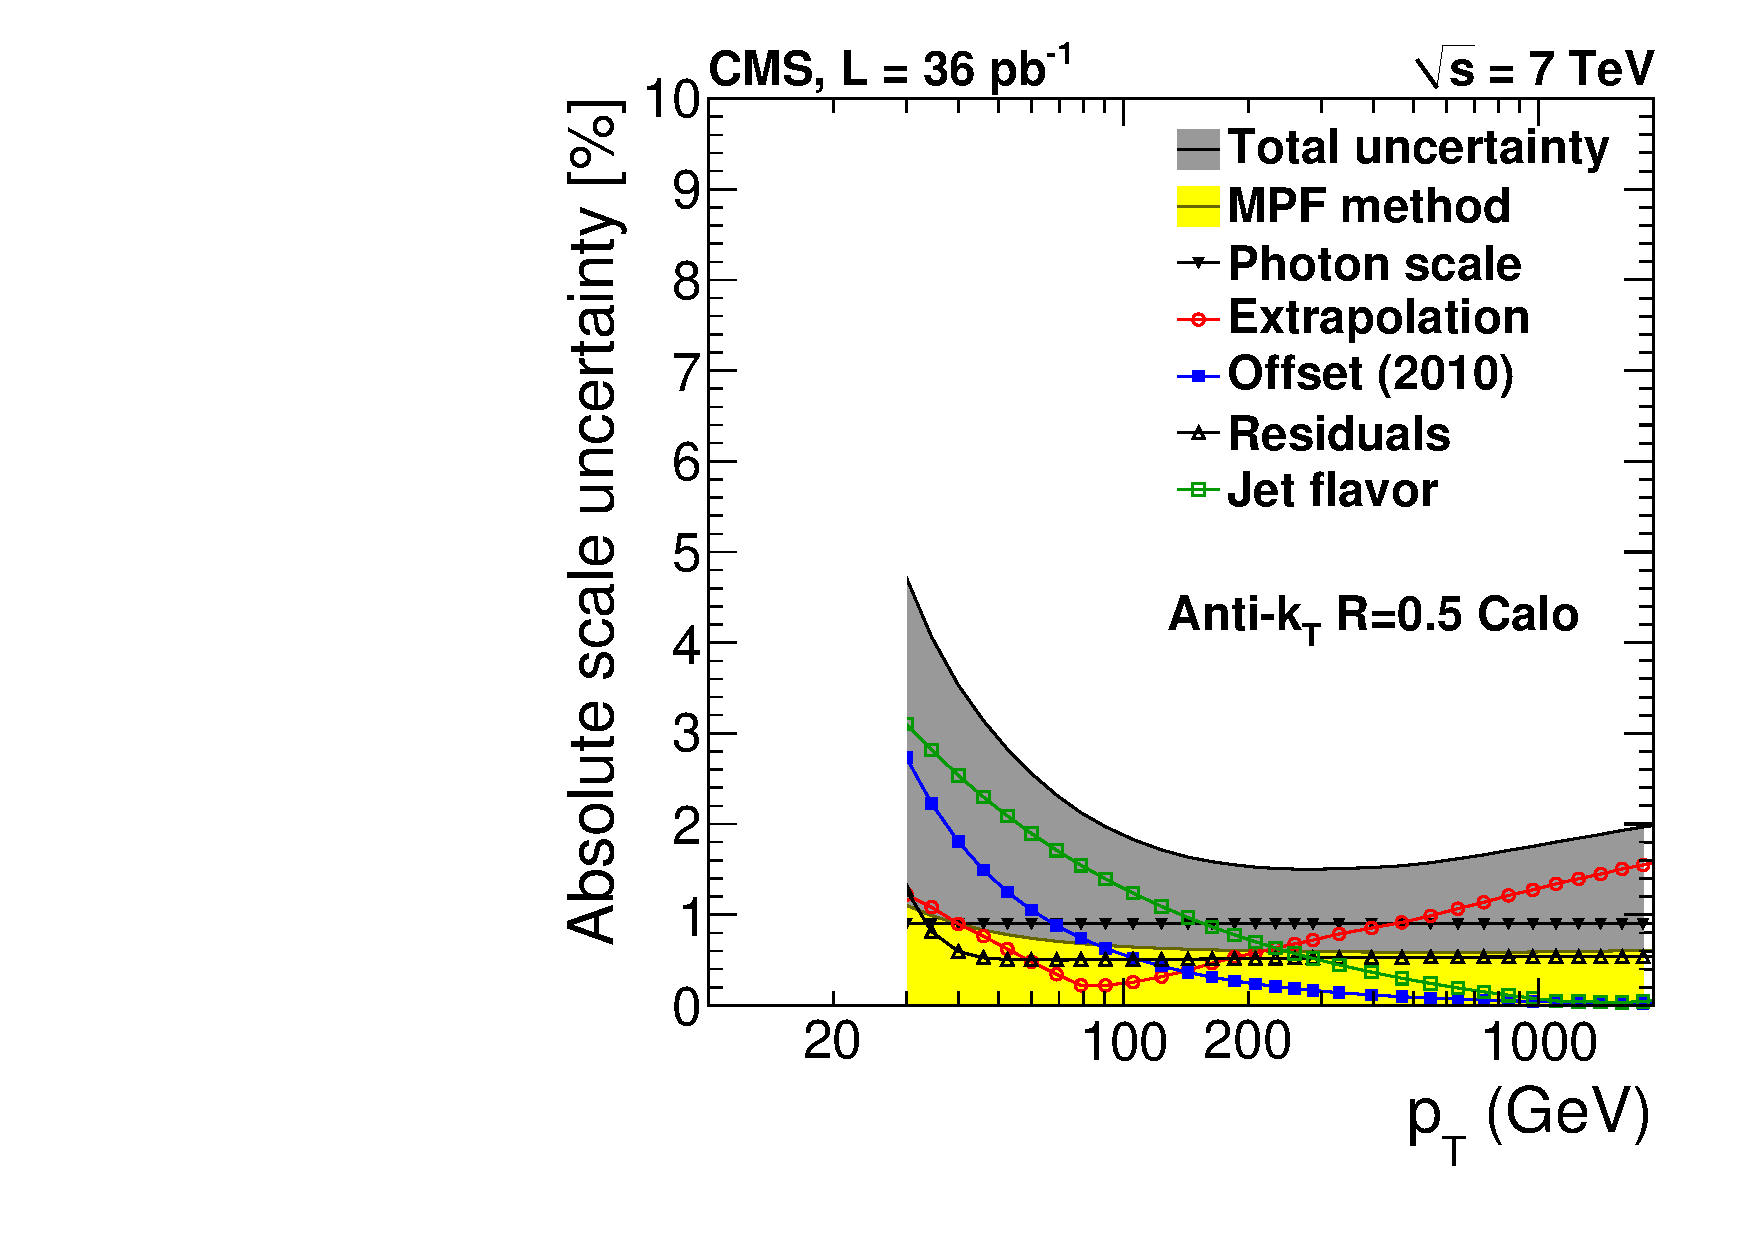
\includegraphics[width=0.45\textwidth]{Figures/JEC/JECUncert_AK5_summary}
    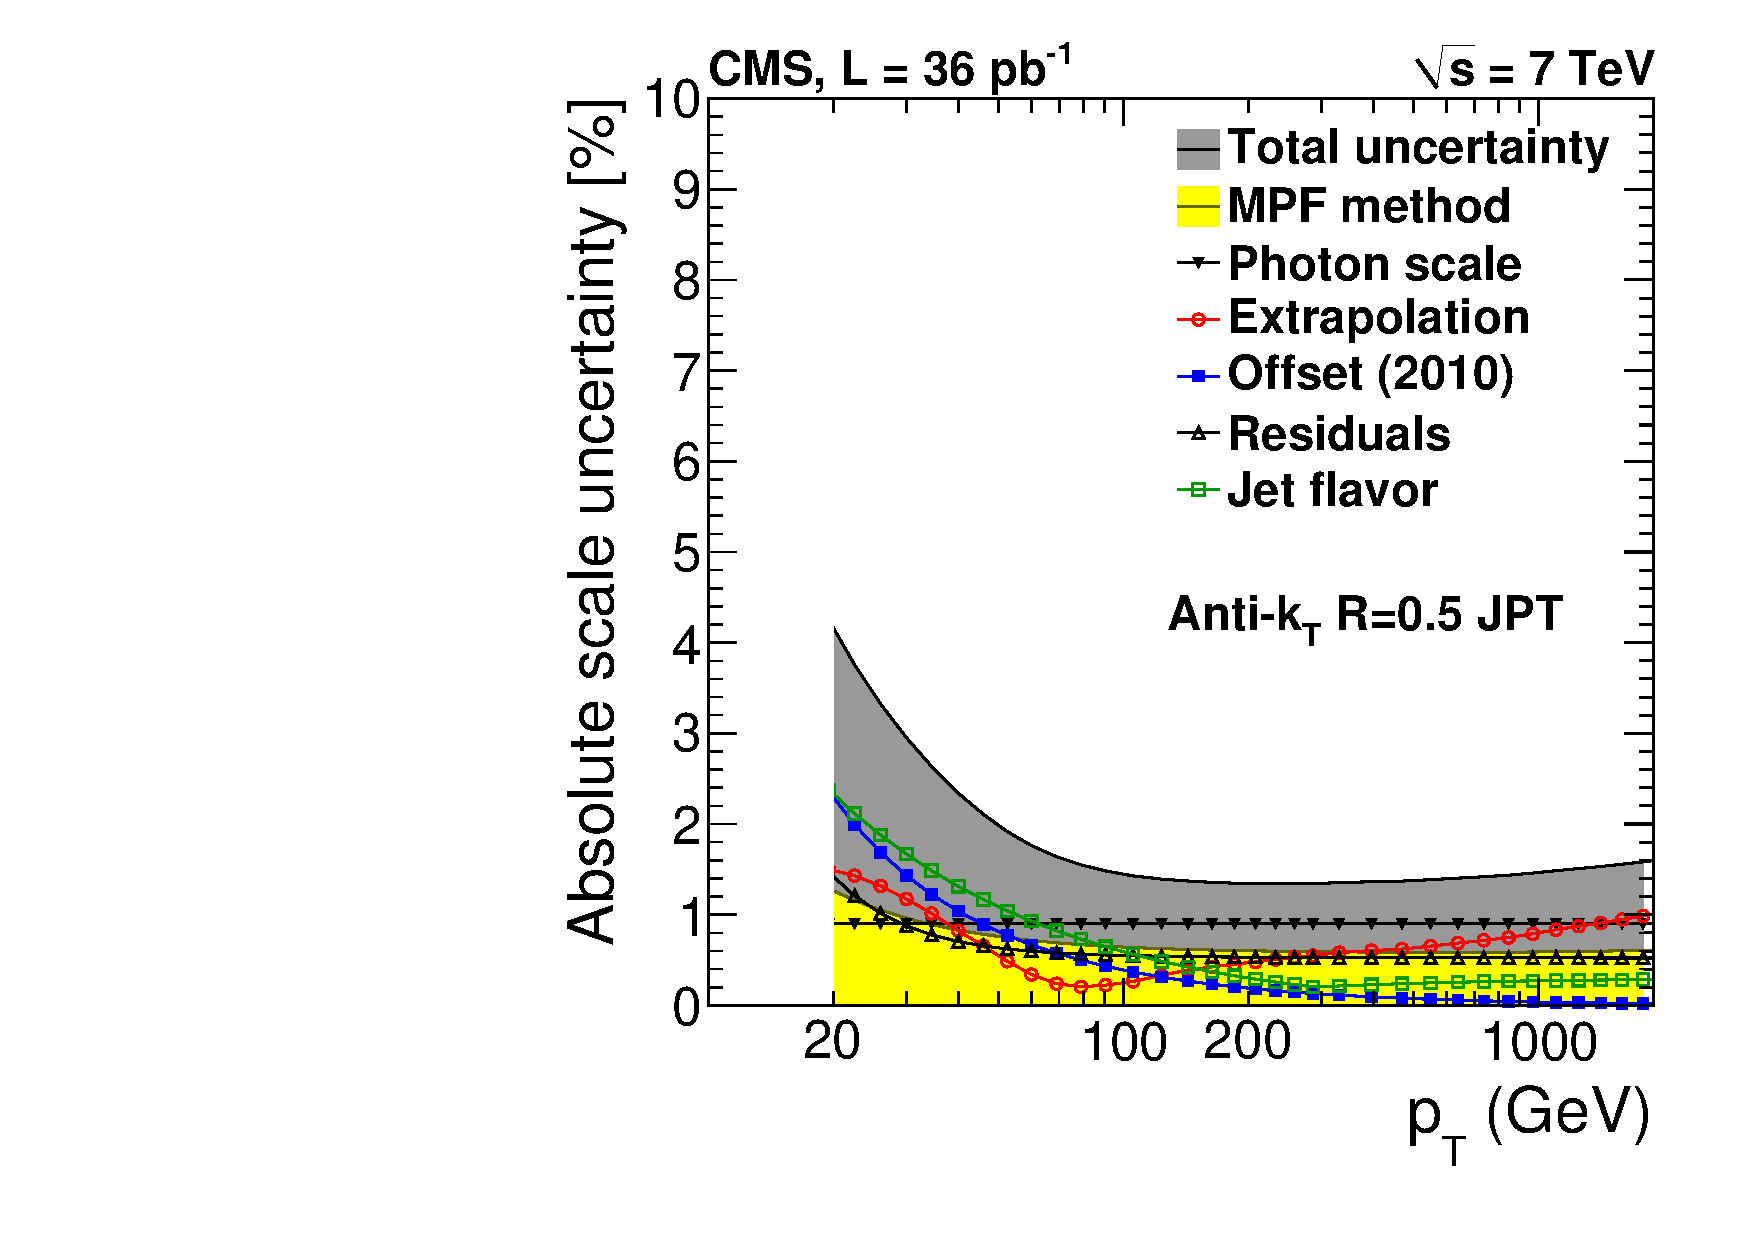
\includegraphics[width=0.45\textwidth]{Figures/JEC/JECUncert_JPTAK5_summary}
    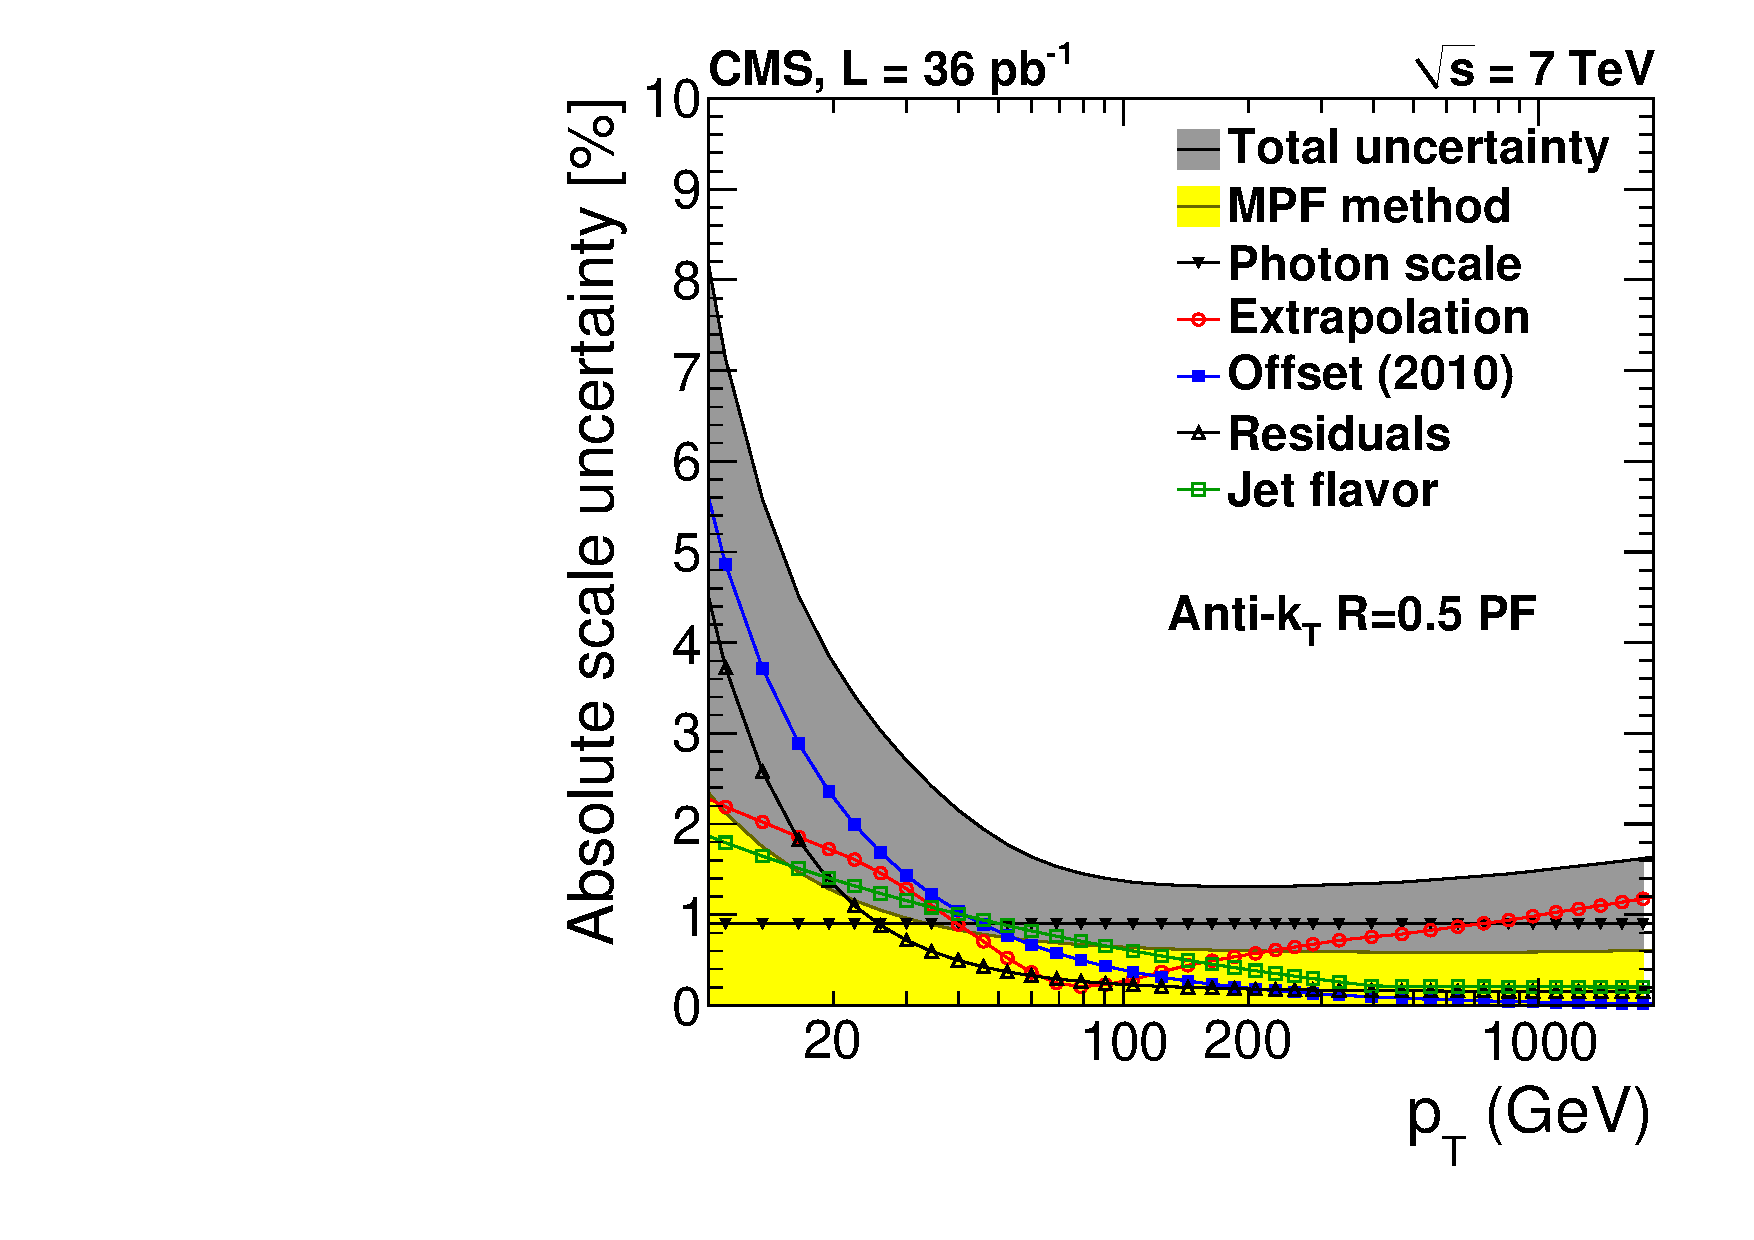
\includegraphics[width=0.45\textwidth]{Figures/JEC/JECUncert_PFAK5_summary}
    \caption{Absolute jet energy scale uncertainty as a function of jet \pt for CALO, JPT and PF jets respectively.}
    \label{fig:absunc}
  \end{center}
\end{figure}

\clearpage

\subsection{Combined Jet Energy Correction}

In this section, the combined MC and residual calibration is presented along with the total jet energy scale systematic uncertainty. Following Eq.~(\ref{eq:jec_components}), the residual corrections for the relative and absolute response are multiplied with the generator-level MC correction, while the corresponding uncertainties are added in quadrature. Figure~\ref{fig:finalJECvsEta} shows the combined calibration factor as a function of jet-$\eta$ for $\pt=50,\,200\GeV$. Because of the smallness of the residual corrections, the combined correction has the shape of the MC component, shown in Fig.~\ref{fig:mctruthVsEta}. The total correction as a function of jet \pt is shown in Fig.~\ref{fig:finalJECvsPt} for various $\eta$ values. Figure~\ref{fig:finalUncvsPt} shows the total jet energy scale uncertainty as a function of jet \pt. At low jet \pt the relative energy scale uncertainty makes a significant contribution to the total uncertainty while it becomes negligible at high \pt. In the forward region, the relative scale uncertainty remains significant in the entire \pt-range. In general PF jets have the smallest systematic uncertainty while CALO jets have the largest.

\begin{figure}[ht!]
  \begin{center}
    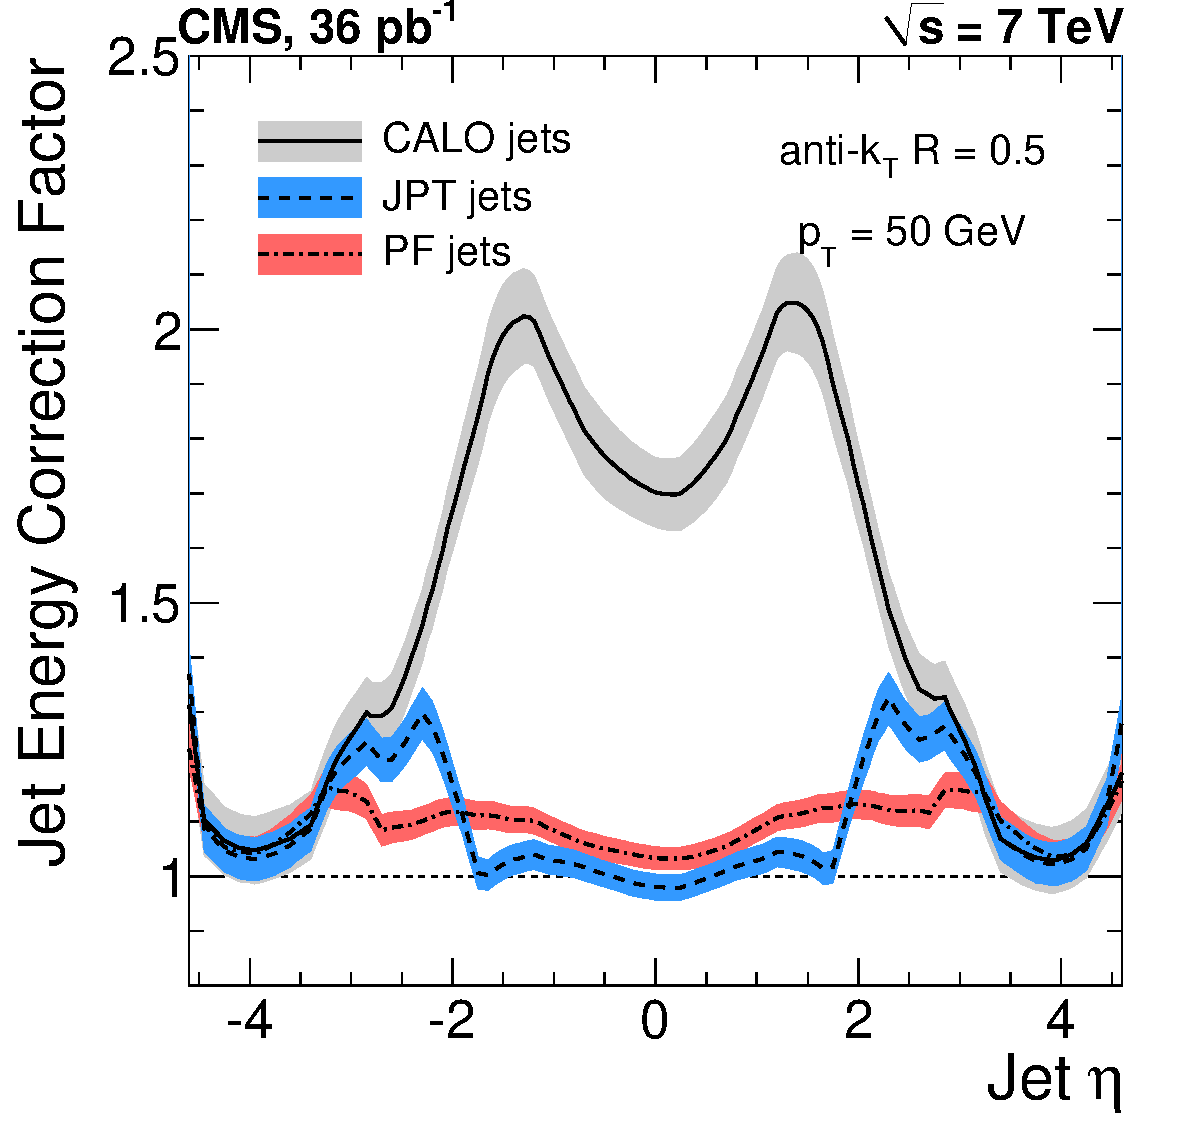
\includegraphics[width=0.45\textwidth]{Figures/JEC/JEC_vs_Eta_CorPt50}
    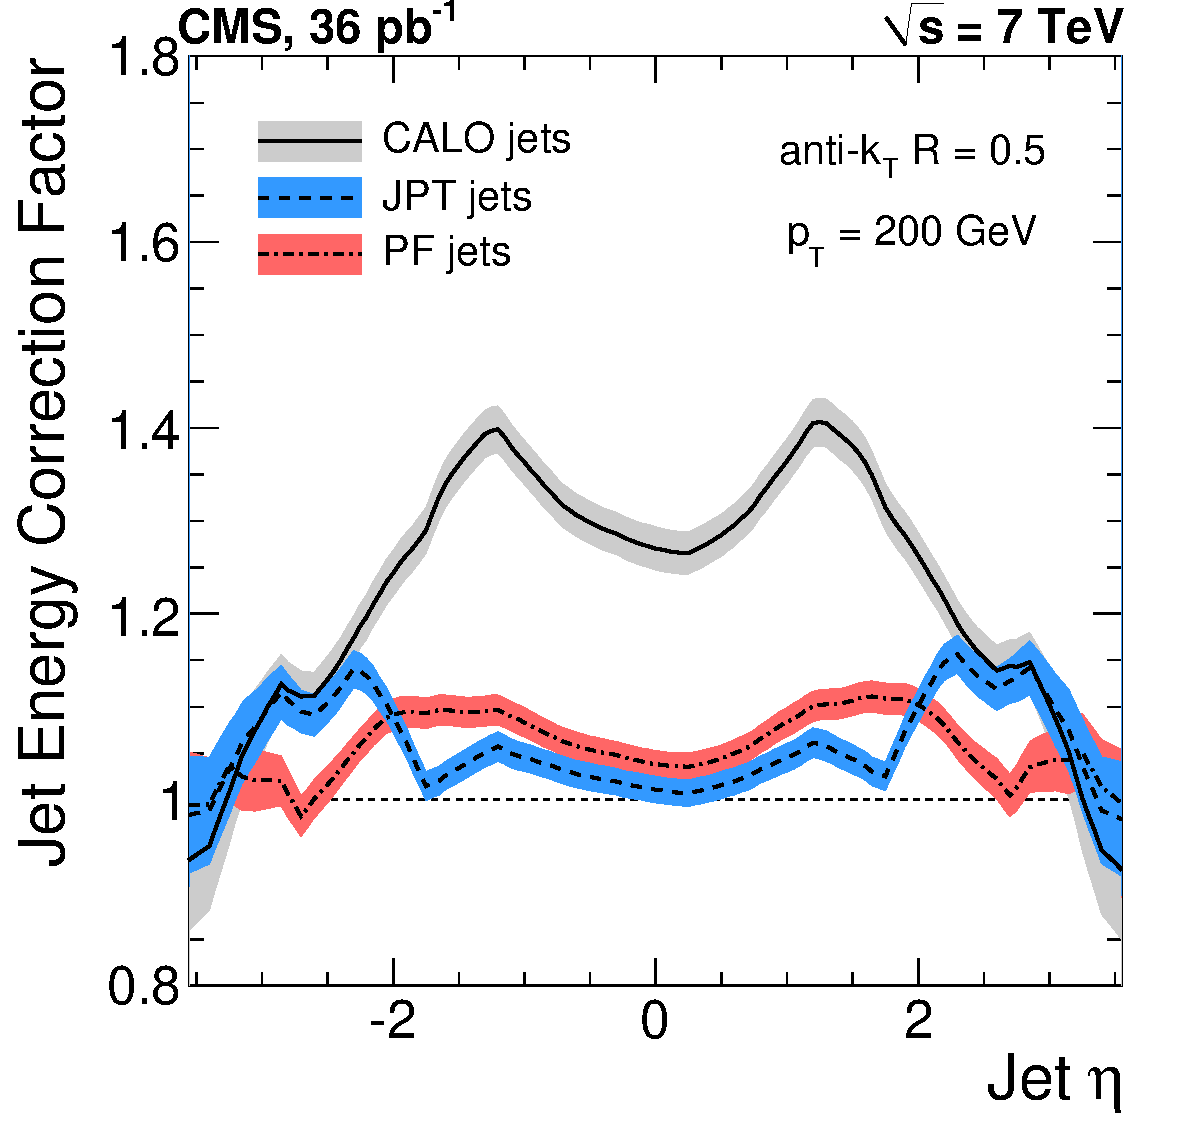
\includegraphics[width=0.45\textwidth]{Figures/JEC/JEC_vs_Eta_CorPt200}
    \caption{Total jet-energy-correction factor, as a function of jet $\eta$ for $\pt=50\GeV$ (left) and $\pt=200\GeV$ (right). The bands indicate the corresponding uncertainty.}
    \label{fig:finalJECvsEta}
  \end{center}
\end{figure}

\begin{figure}[ht!]
  \begin{center}
    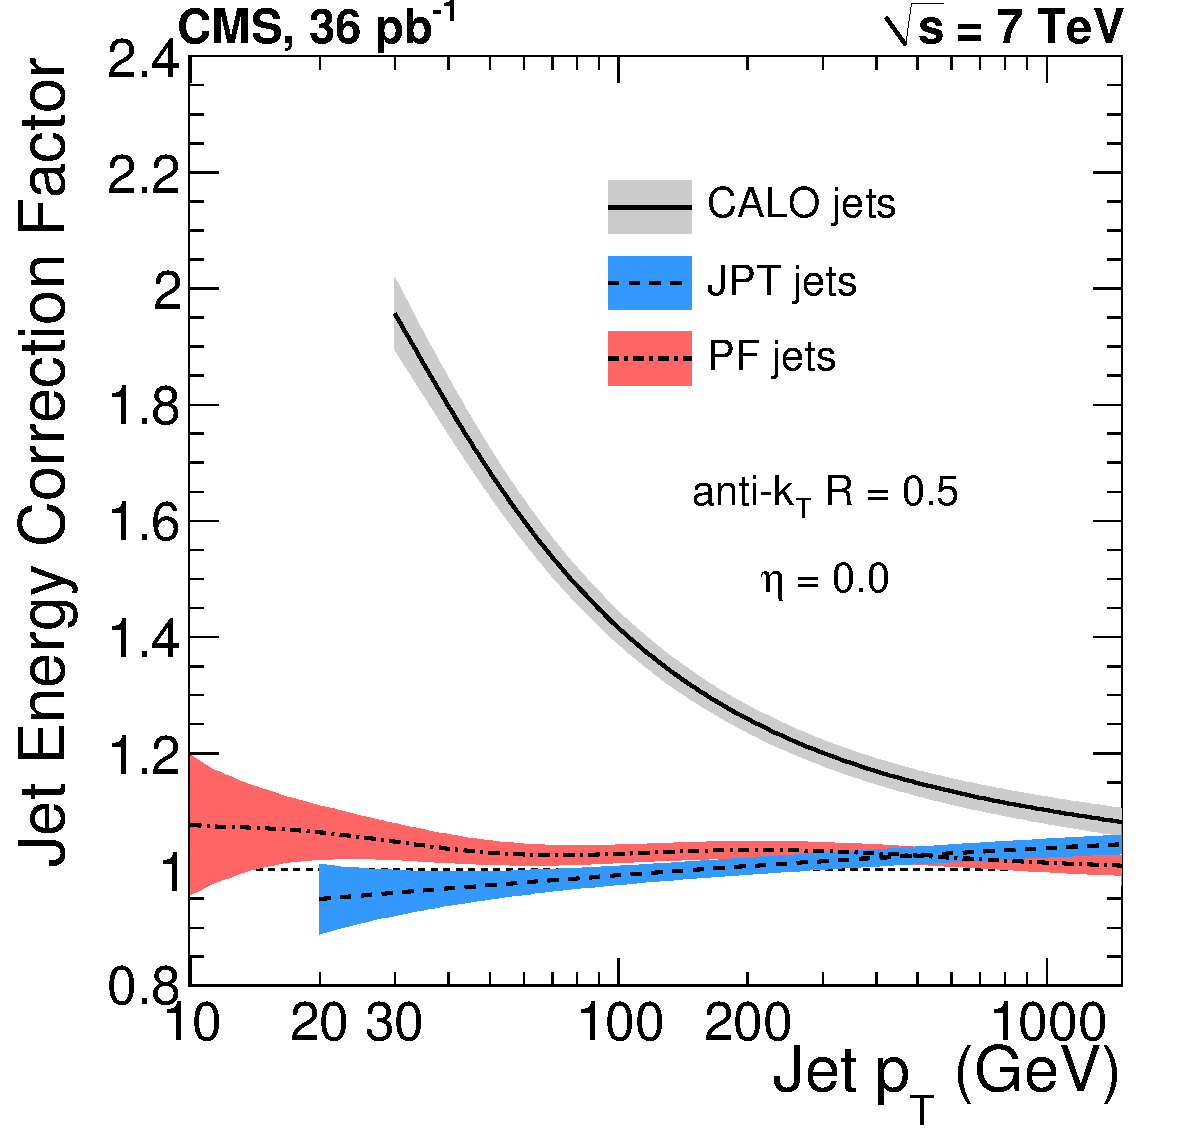
\includegraphics[width=0.45\textwidth]{Figures/JEC/JEC_vs_CorPt_eta0}
    \includegraphics[width=0.45\textwidth]{Figures/JEC/JEC_vs_CorPt_eta10}
    \includegraphics[width=0.45\textwidth]{Figures/JEC/JEC_vs_CorPt_eta20}
    \includegraphics[width=0.45\textwidth]{Figures/JEC/JEC_vs_CorPt_eta40}
    \caption{Total jet-energy-correction factor, as a function of jet \pt for various $\eta$ values. The bands indicate the corresponding uncertainty.}
    \label{fig:finalJECvsPt}
  \end{center}
\end{figure}

\begin{figure}[ht!]
  \begin{center}
    \includegraphics[width=0.45\textwidth]{Figures/JEC/Uncertainty_Eta0}
    \includegraphics[width=0.45\textwidth]{Figures/JEC/Uncertainty_Eta20}
    \includegraphics[width=0.45\textwidth]{Figures/JEC/Uncertainty_Eta40}
    \caption{Total jet-energy-scale uncertainty, as a function of jet \pt for various $\eta$ values.}
    \label{fig:finalUncvsPt}
  \end{center}
\end{figure}


























